\documentclass[10pt]{beamer}

\usetheme[progressbar=frametitle]{metropolis}
\usepackage{appendixnumberbeamer}

\usepackage{booktabs}
\usepackage[scale=2]{ccicons}

\usepackage{pgfplots}
\usepgfplotslibrary{dateplot}

\usepackage{xspace}
\newcommand{\themename}{\textbf{\textsc{metropolis}}\xspace}

\usepackage{bibentry}

\title{Uni- and Multivariate Analysis of Dendritic Ca2+ Data}
\subtitle{In a Stimulus Detection Task}
\date{\today}
%\date{}
\author{Georg Chechelnizki}
\institute{BCCN Berlin}
% \titlegraphic{\hfill\includegraphics[height=1.5cm]{logo.pdf}}

\setbeamercolor{background canvas}{bg=white}
\usepackage{caption}

\begin{document}

\maketitle

\begin{frame}{Table of contents}
  \setbeamertemplate{section in toc}[sections numbered]
  \tableofcontents[hideallsubsections]
\end{frame}

\section{Introduction}

\begin{frame}[fragile]{The Experiment}
Takahashi et al. 2016	
\begin{columns}[T,onlytextwidth]
    \column{0.5\textwidth}
    	\only<+->{
      \begin{figure}
      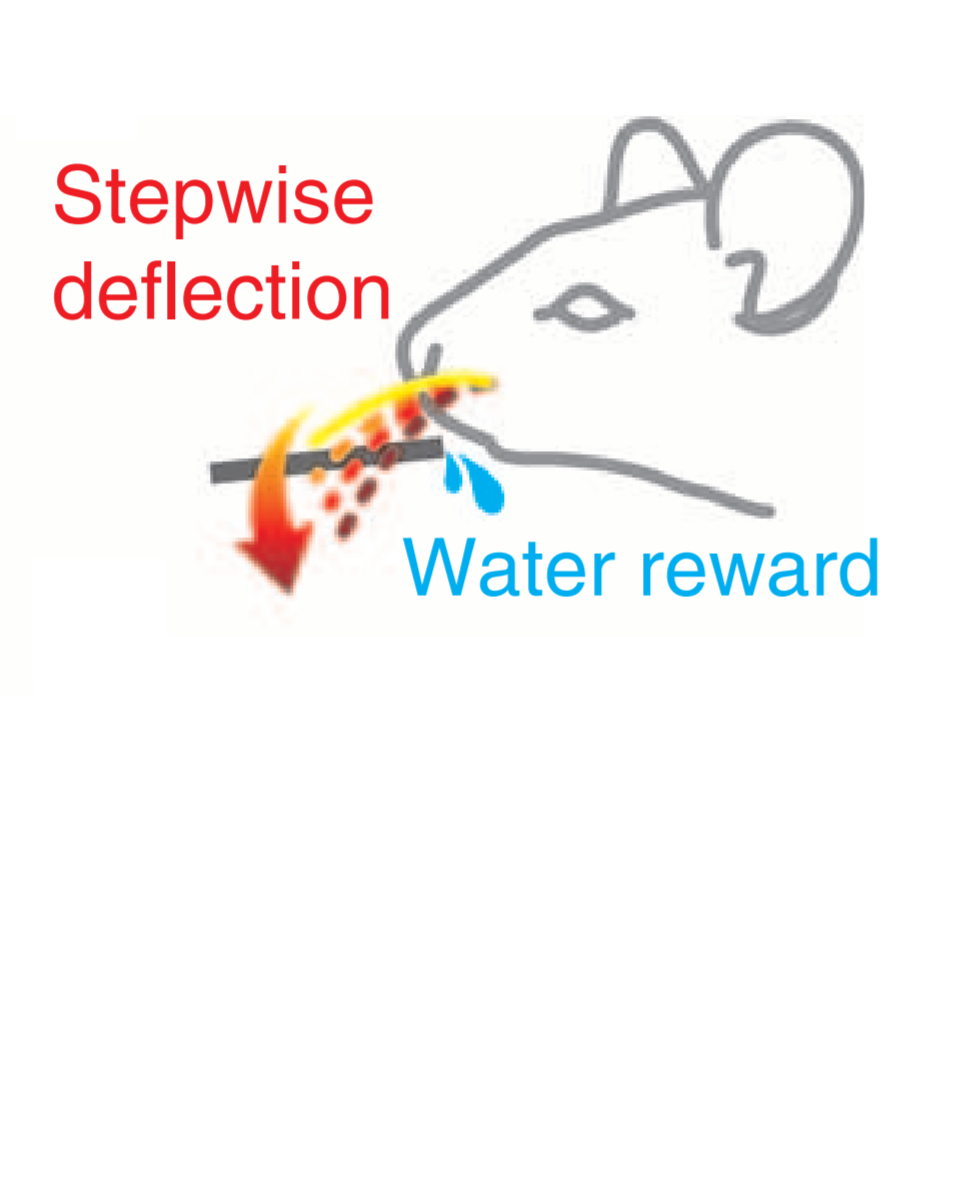
\includegraphics[scale=0.1]{mouse.png}
      \end{figure}}
      
    \column{0.5\textwidth}
		\only<+->{
      \begin{figure}
      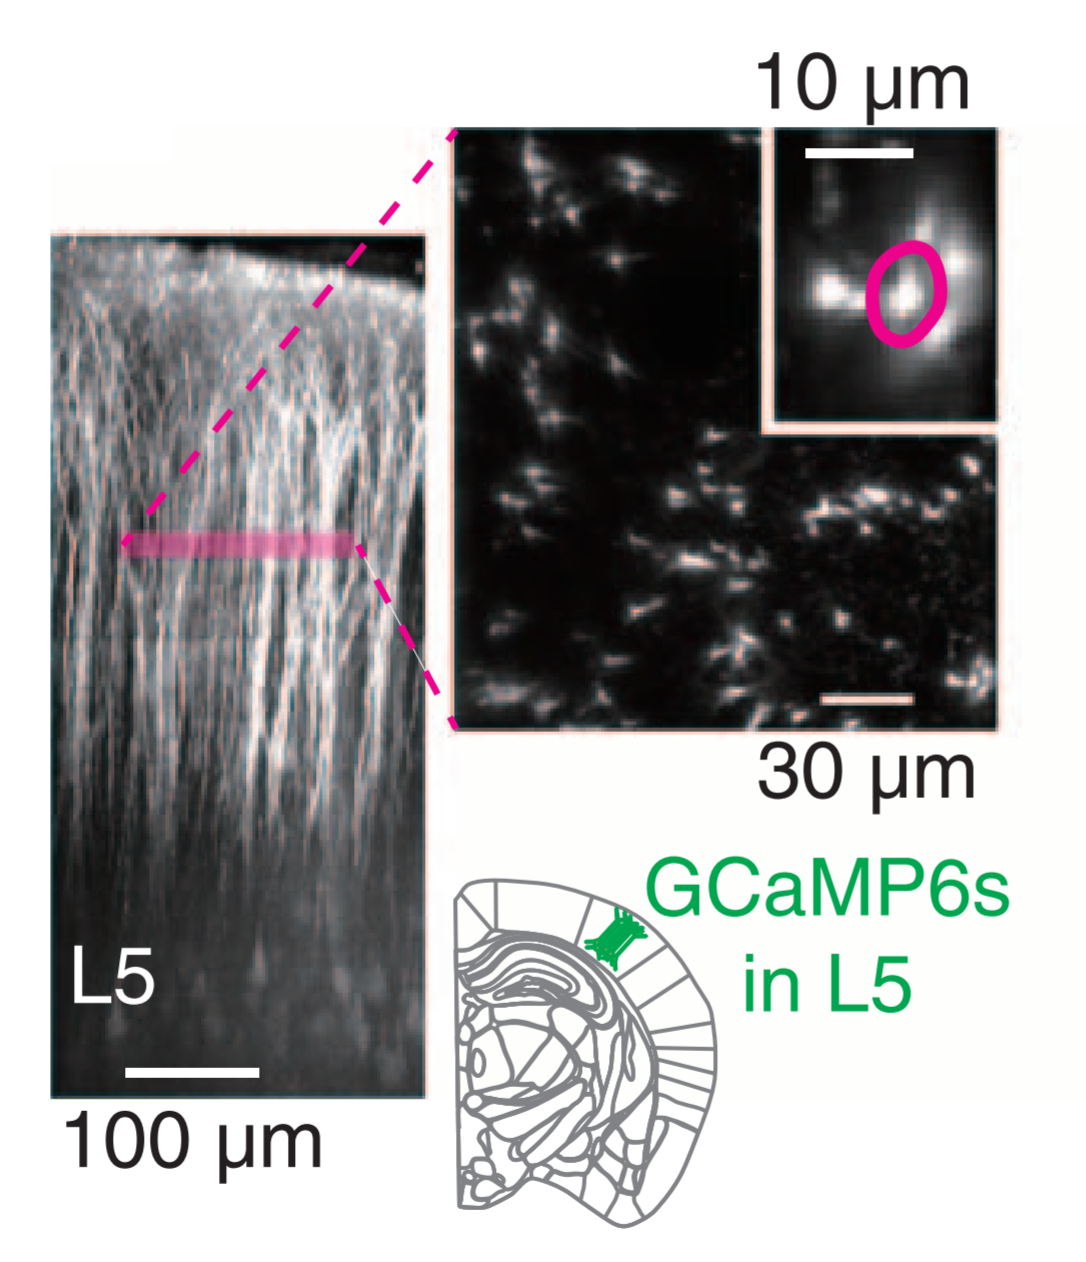
\includegraphics[scale=0.1]{roi.png}
      \end{figure}}

  \end{columns}
\end{frame}

\begin{frame}[fragile]{The Data - Neuronal}
	\begin{center}
	\begin{figure}
	\caption*{Trial-averaged $\text{Ca}^{2+}$ fluorescence traces of random dendrites}
      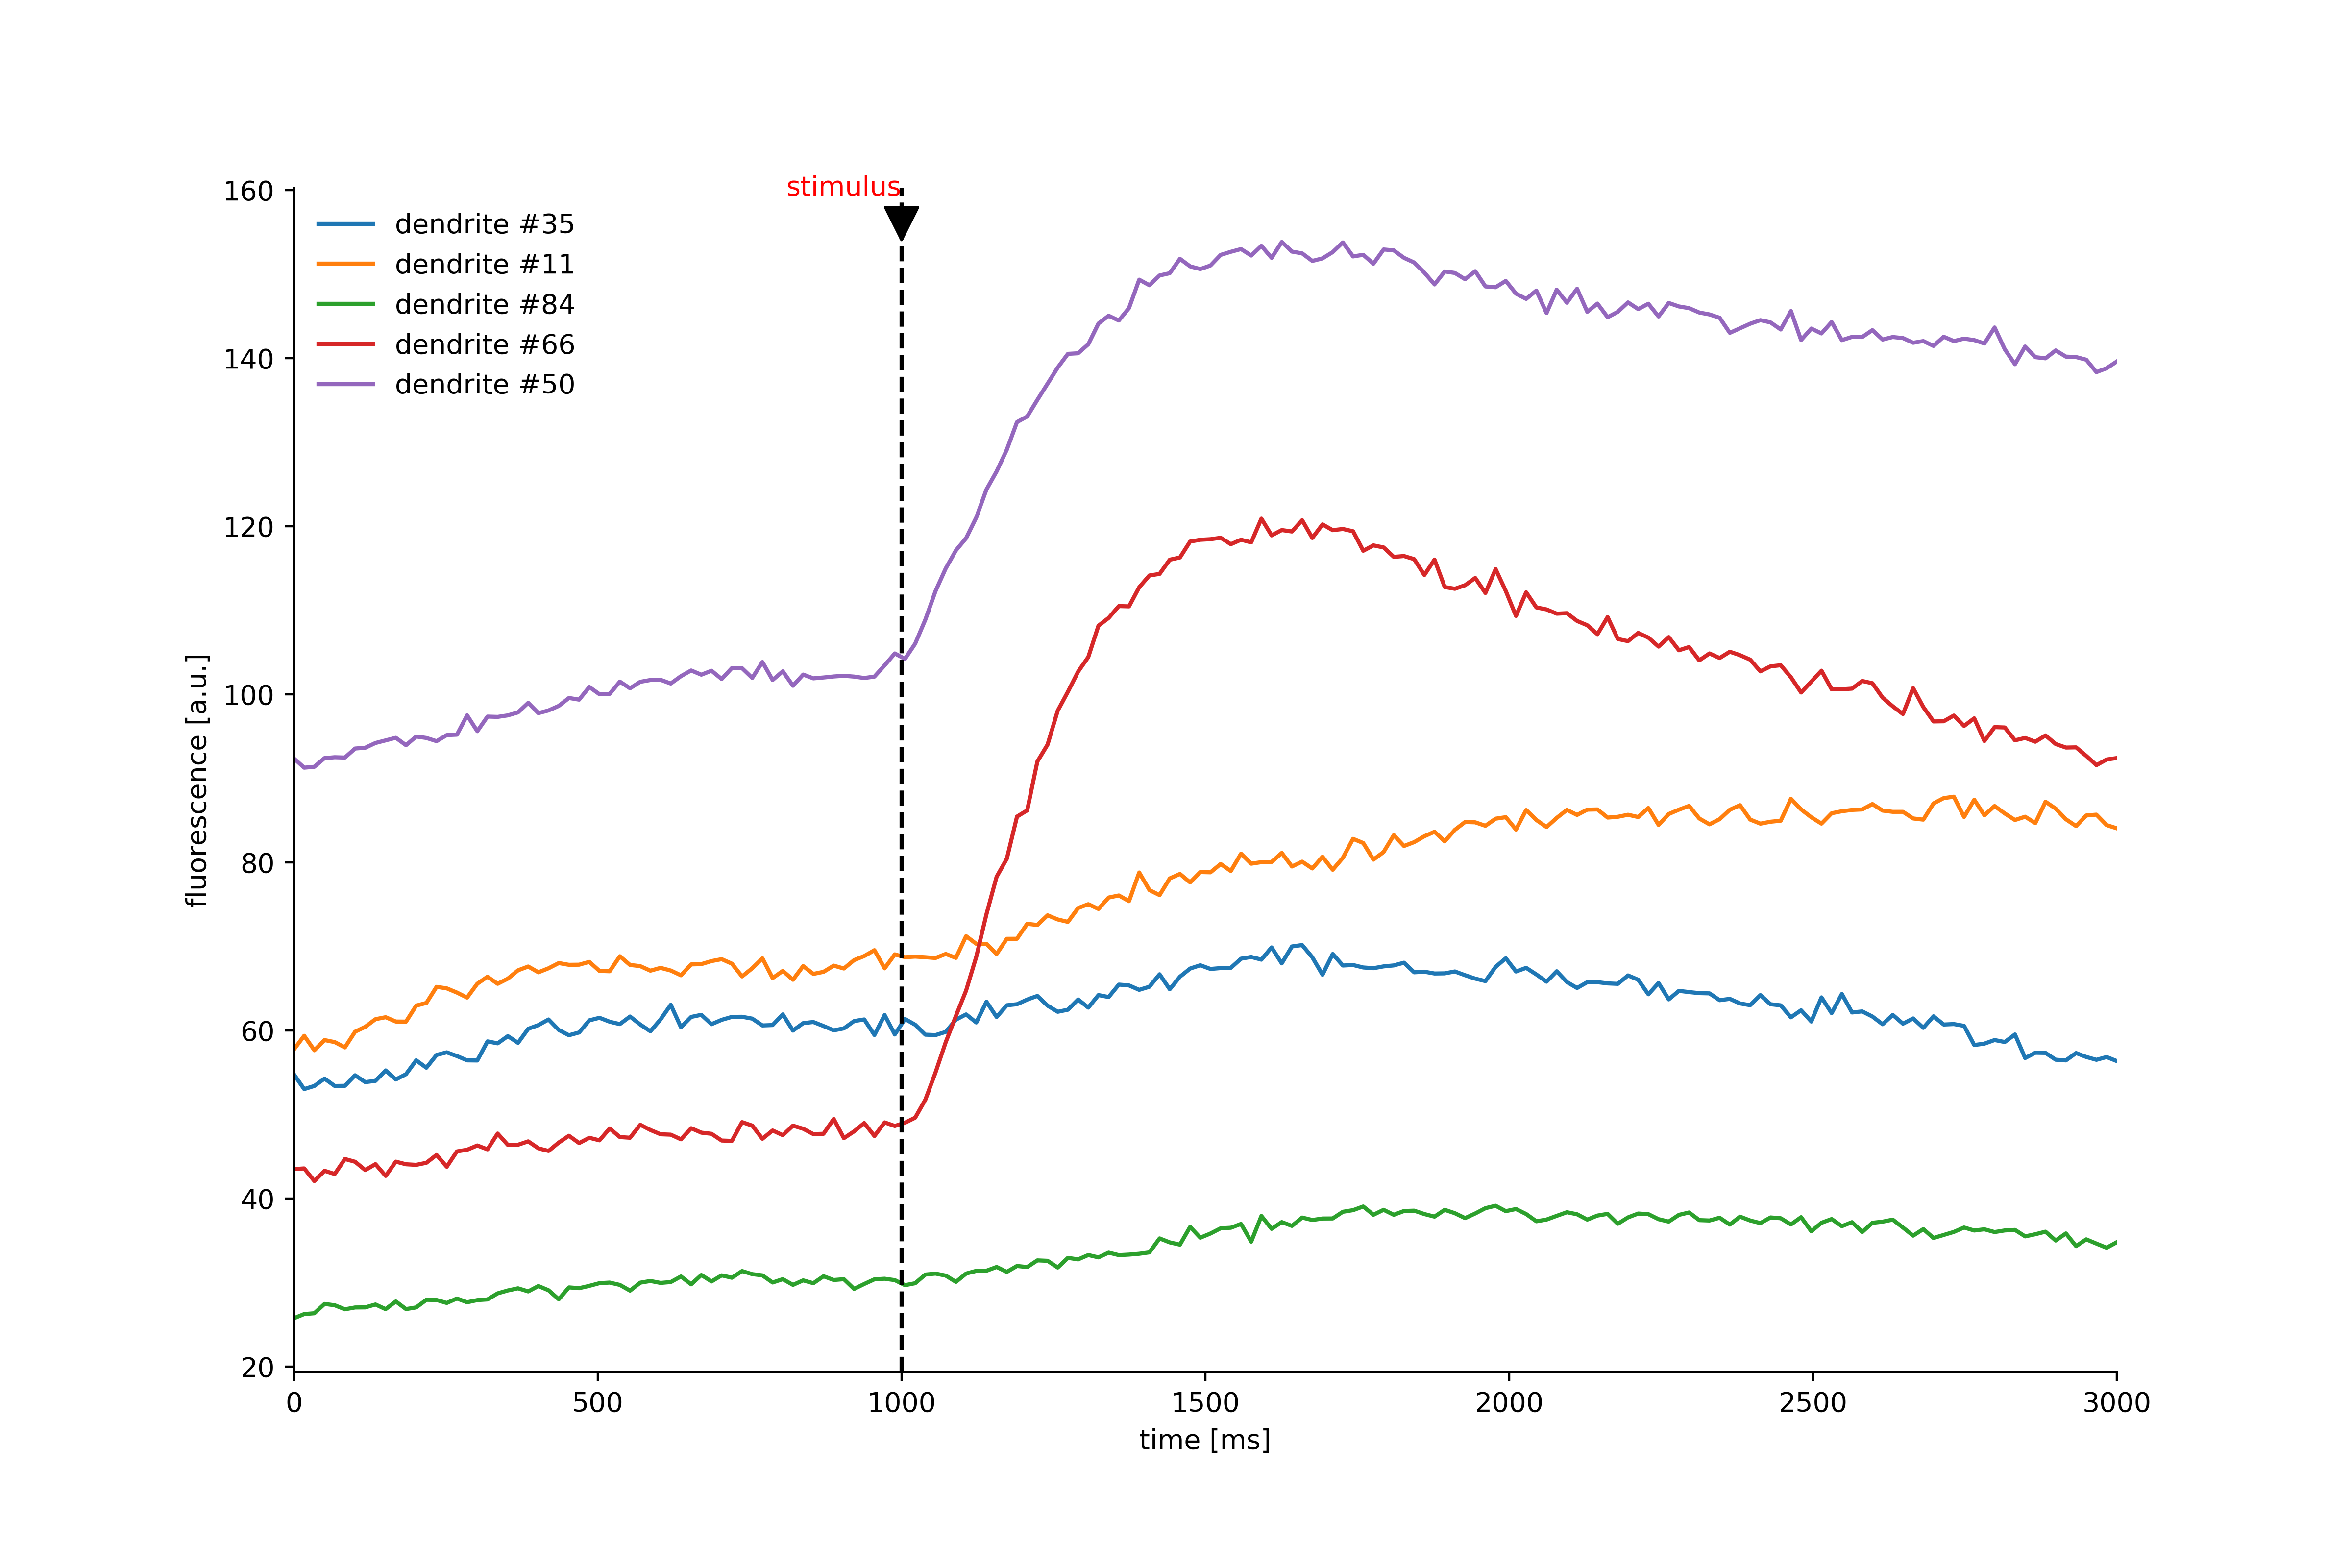
\includegraphics[width=\textwidth]{traces.png}
	\end{figure}
	\end{center}
\end{frame}

\begin{frame}[fragile]{The Data - Neuronal}
	\begin{center}
	\begin{figure}
	\caption*{Trial-averaged $\text{Ca}^{2+}$ fluorescence traces of random dendrites}
      \includegraphics[width=\textwidth]{traces_roi.png}
	\end{figure}
	\end{center}
\end{frame}

\begin{frame}[fragile]{The Data - Behavioral}
	\begin{center}
	\begin{figure}
      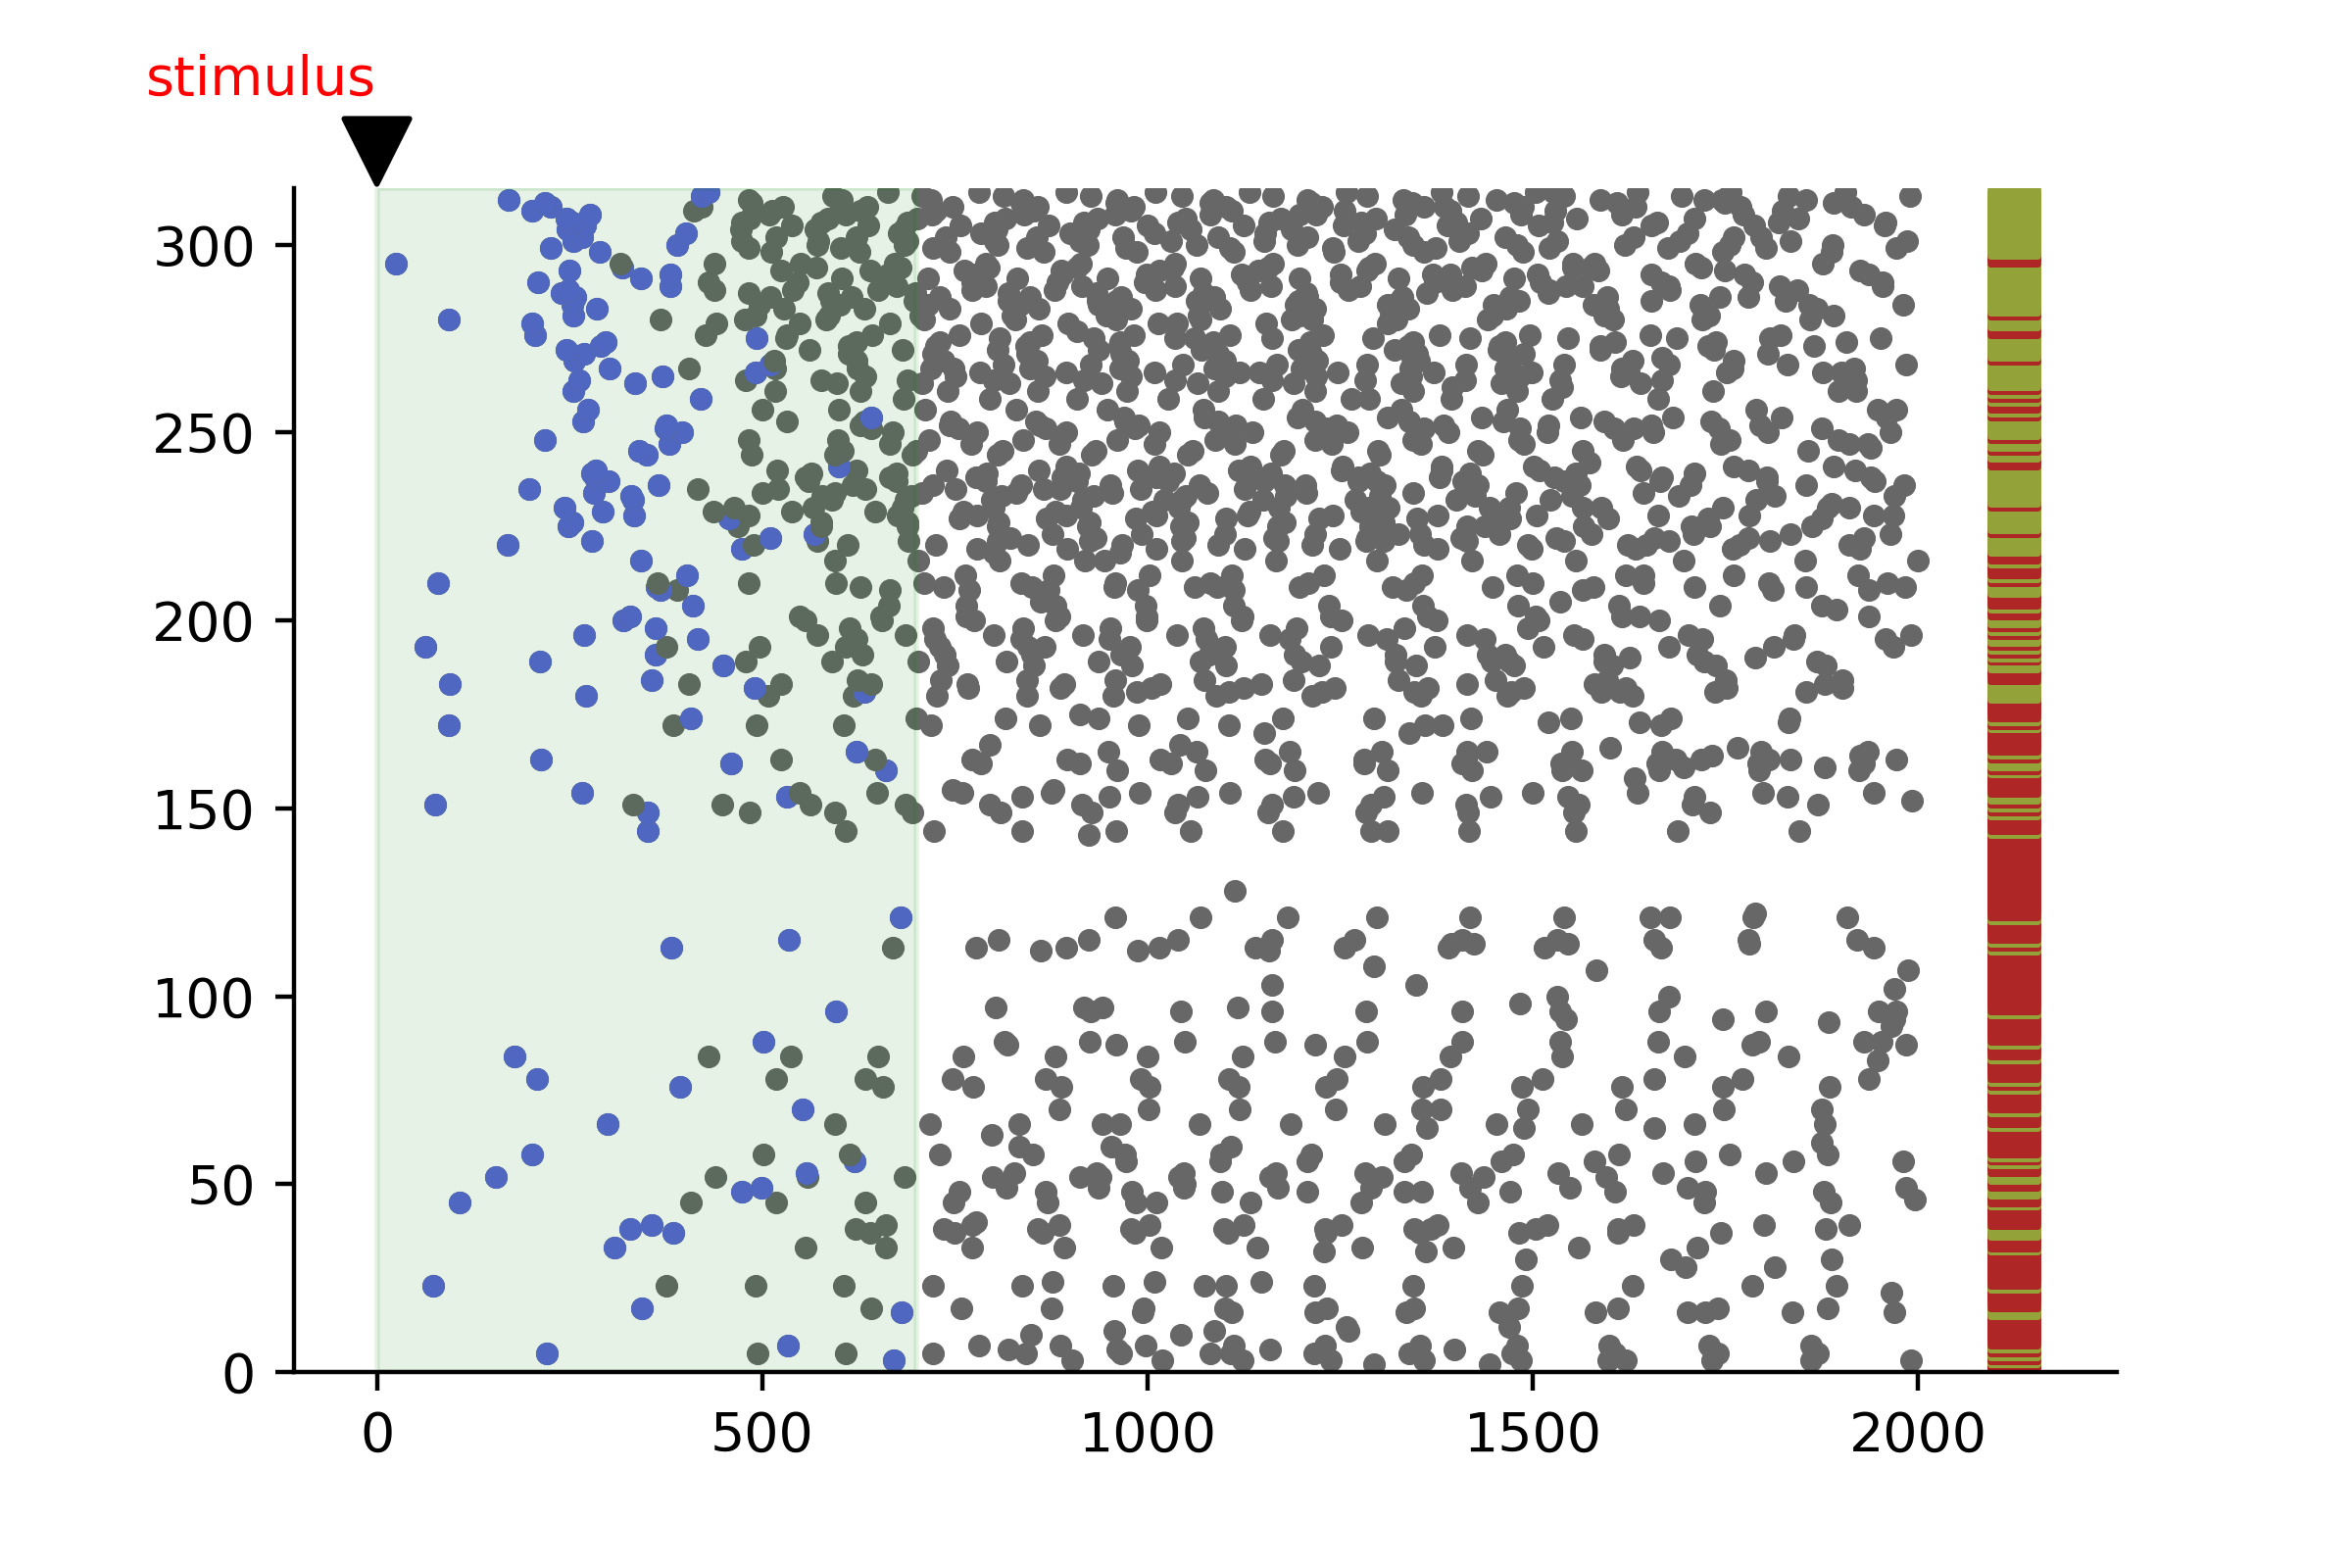
\includegraphics[width=\textwidth]{lickplot_single.png}
	\end{figure}
	\end{center}
\end{frame}

\begin{frame}[fragile]{The Data - Psychometric Curve}
\begin{center}
	\begin{figure}
      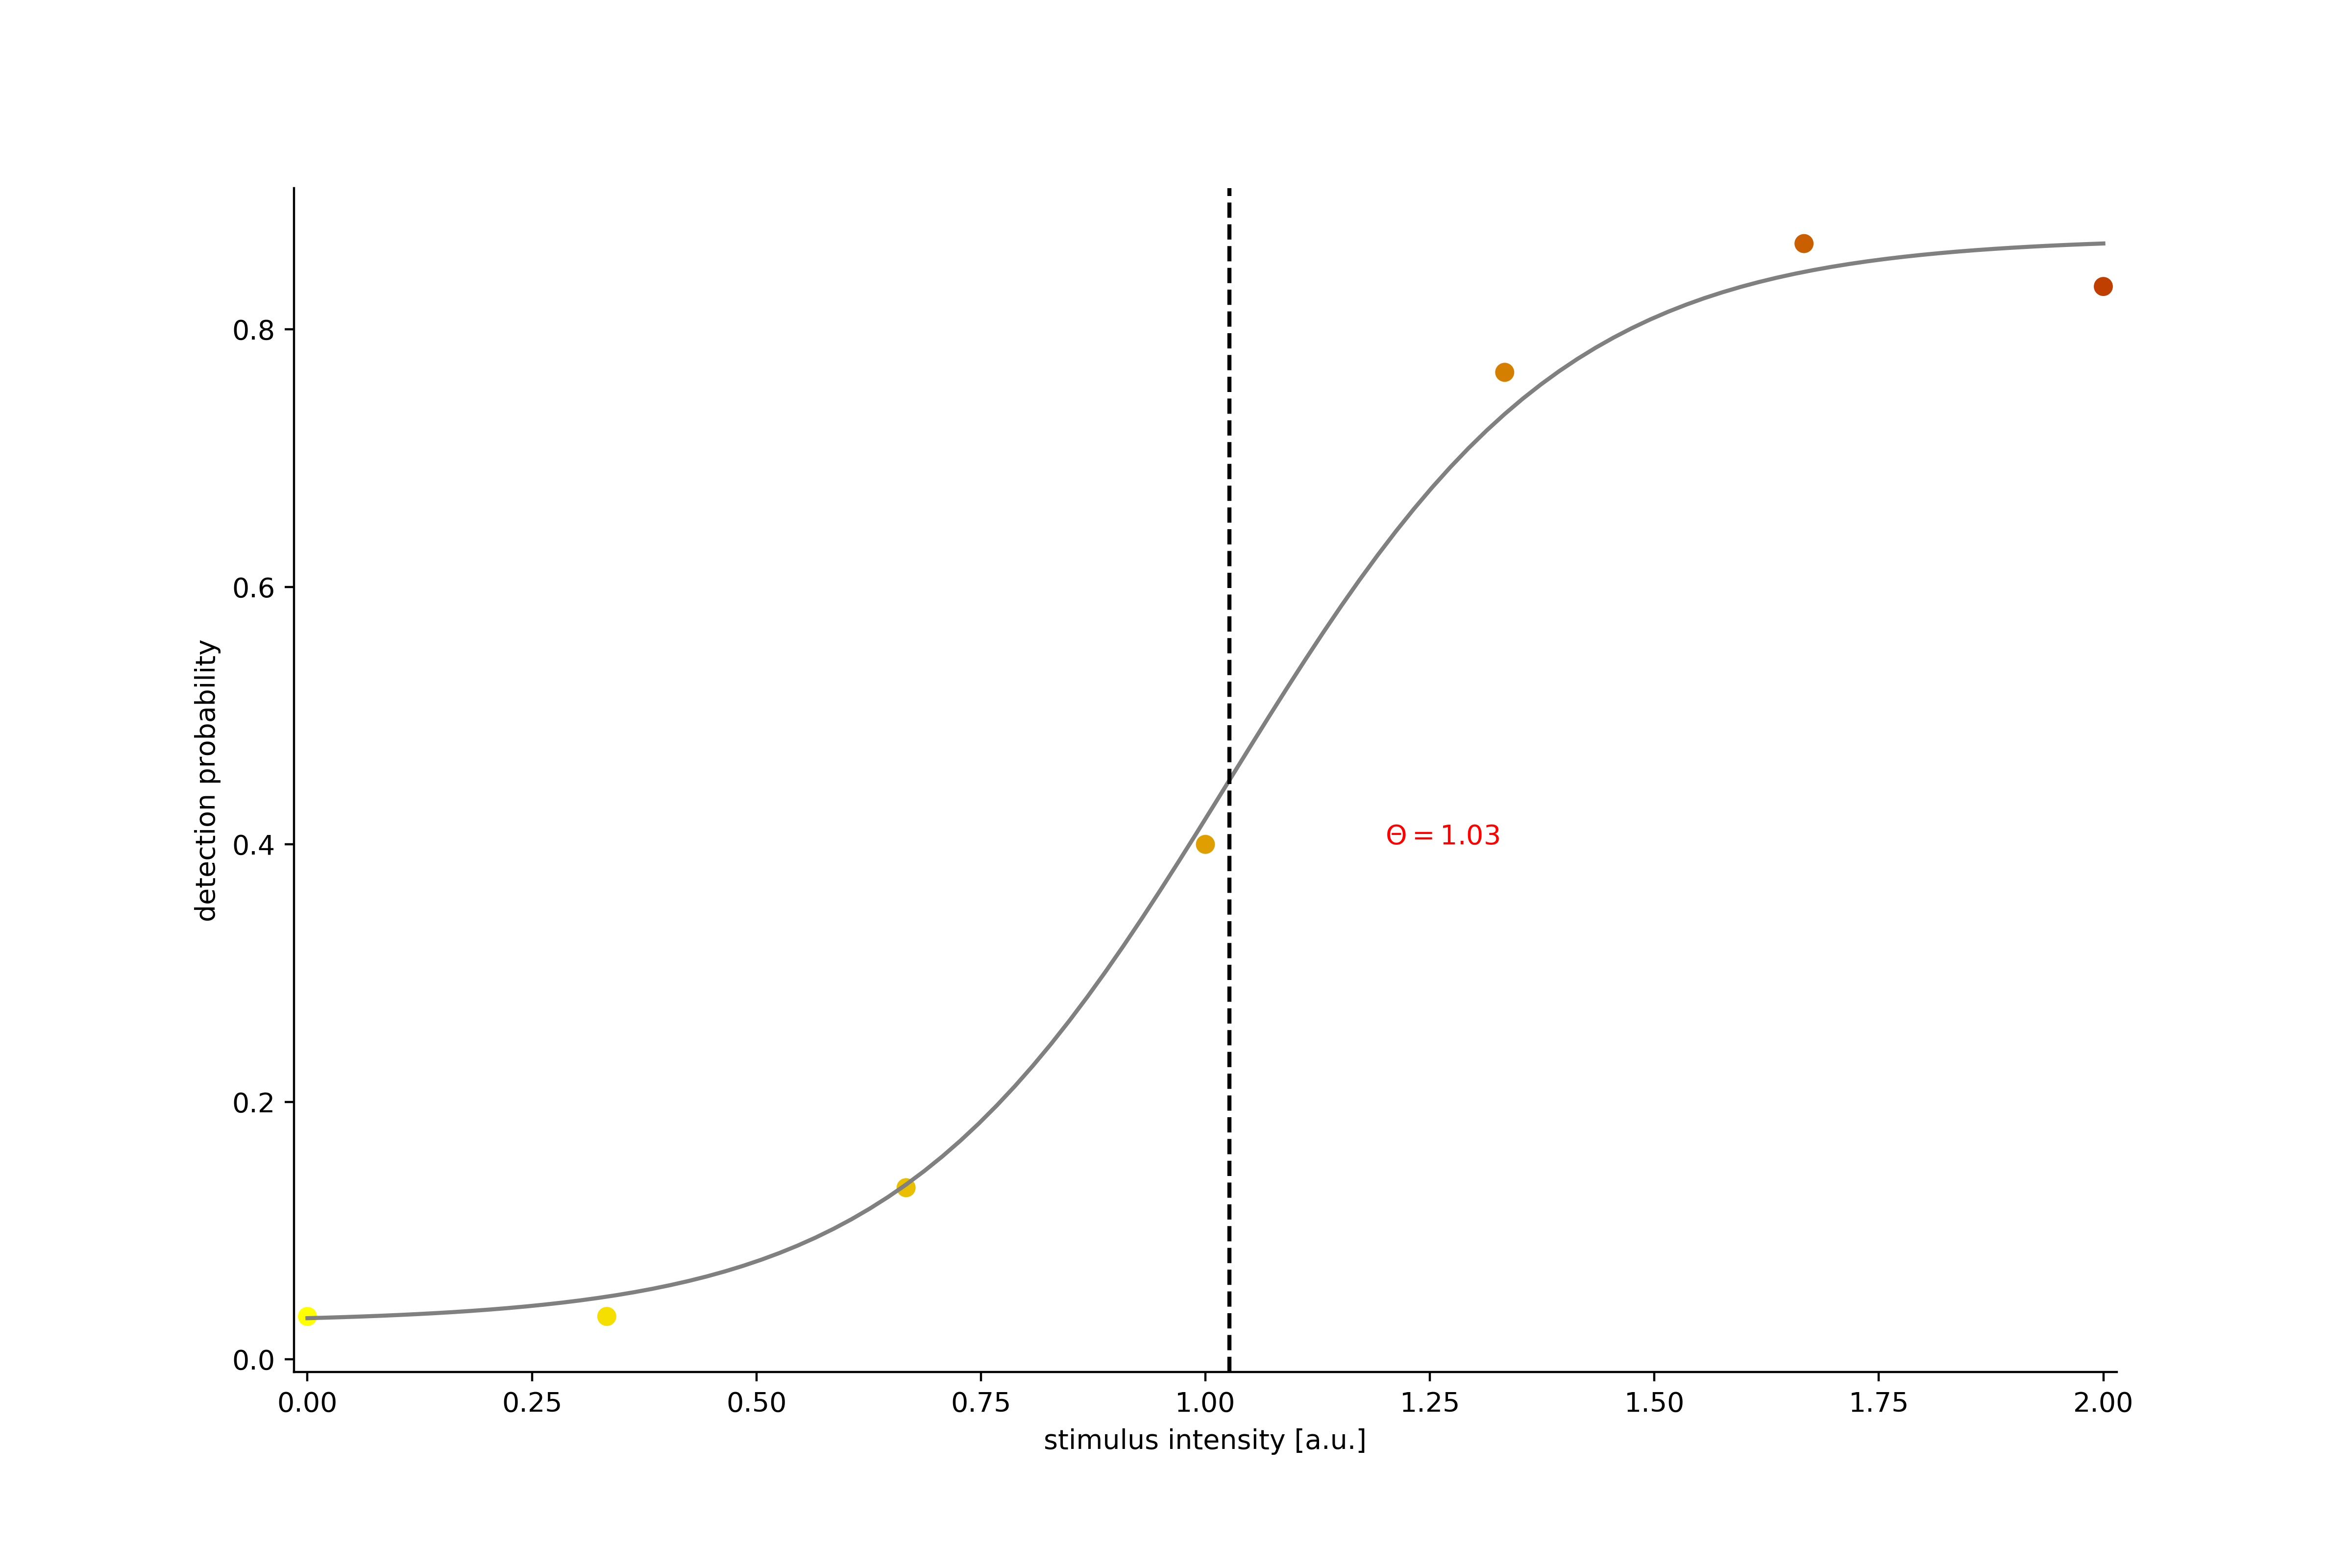
\includegraphics[width=\textwidth]{psychometric.png}
	\end{figure}
	\end{center}
	
\end{frame}

\section{Goal}
\begin{frame}[fragile]{Goal}
The goal of this project is to investigate the following:
\begin{itemize}
\only<+->{
\item What is the relationship between Ca2+ activity and stimulus intensity/behavior}
\only<+->{
\item Does a multivariate approach give us any significant advantage over a univariate one?}
\end{itemize}
\end{frame}

\section{Univariate Analysis}

\begin{frame}[fragile]{Stimulus Presence Detection}
%\begin{itemize}
%\item Feature: mean activity of dendrite over one second after stimulus
%\item Class one: all trials with stimulus strength 0
%\item Class two: all trials with selected stimulus strength $(\neq 0)$
%\end{itemize}
\begin{center}
	\begin{figure}
      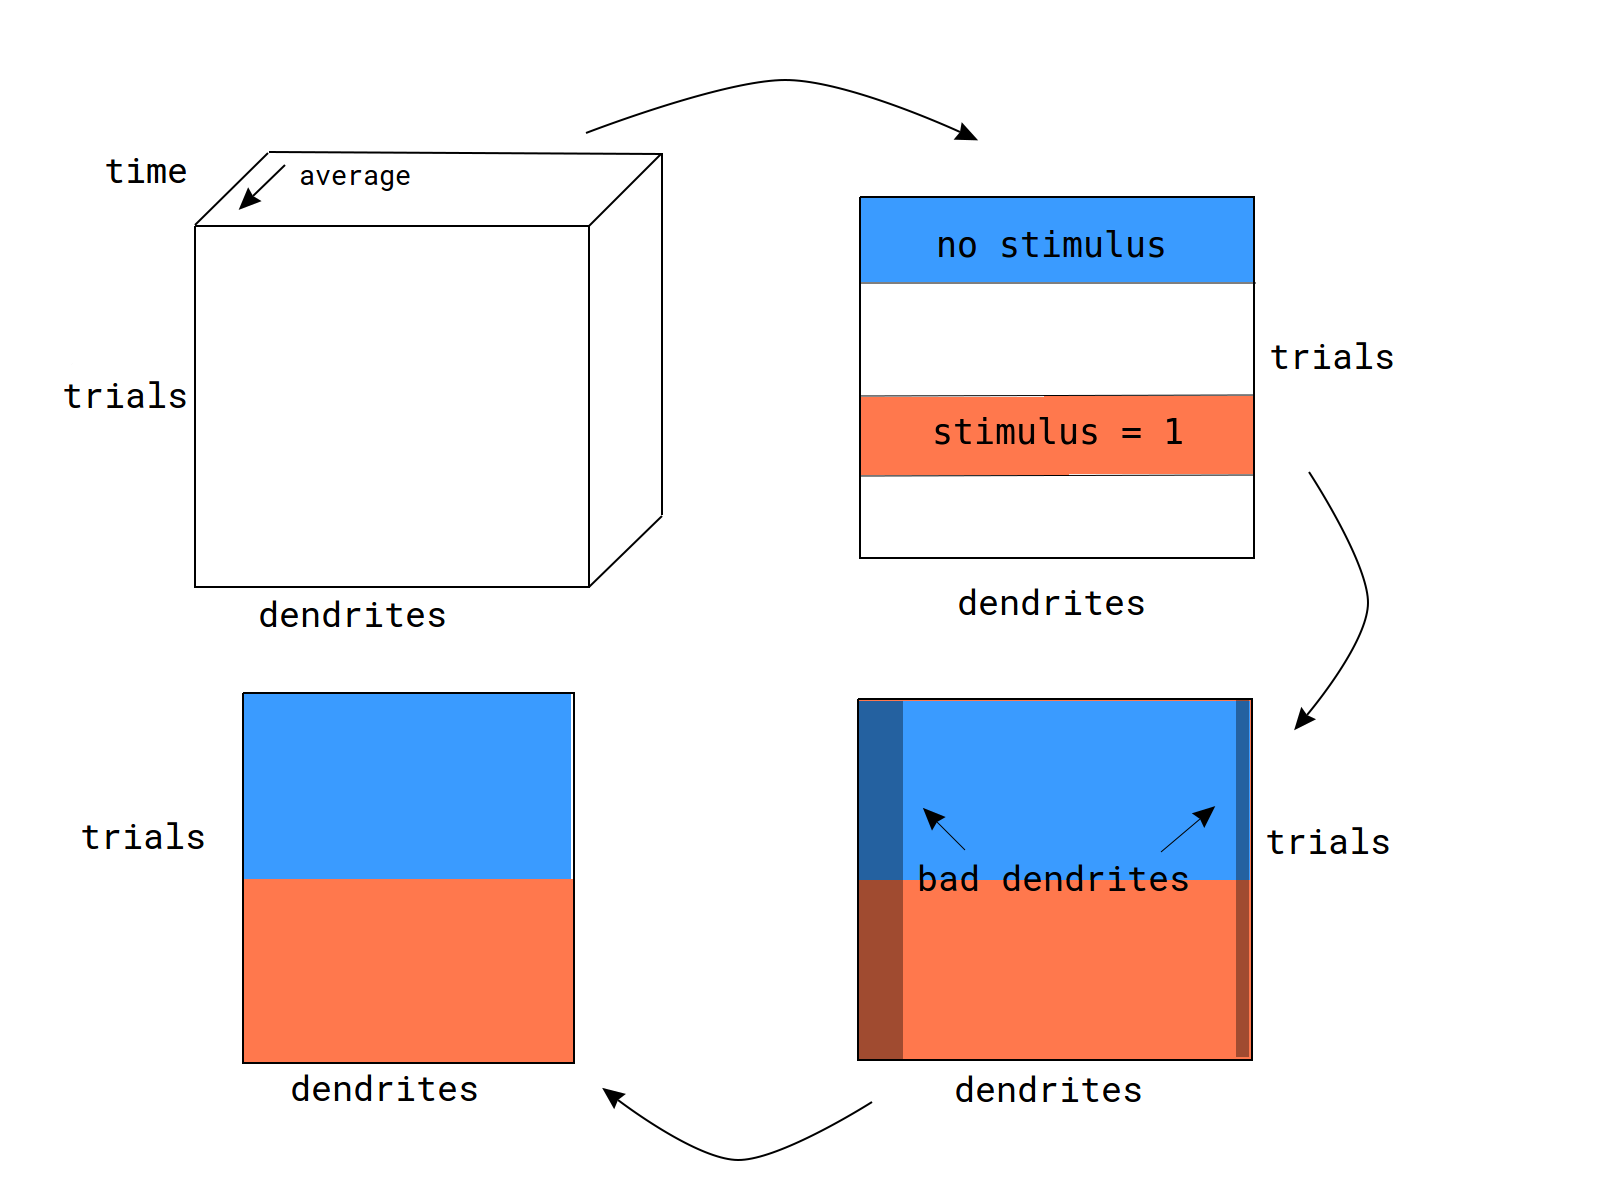
\includegraphics[width=1.0\textwidth]{data_p.png}
	\end{figure}
	\end{center}
\end{frame}

\begin{frame}[fragile]{ROC}
\begin{center}
	\begin{figure}
      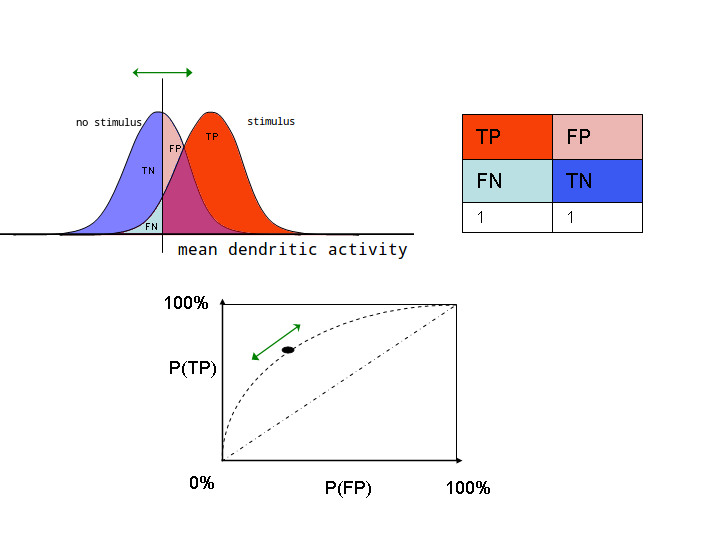
\includegraphics[width=1.0\textwidth]{roc_exp.png}
	\end{figure}
	\end{center}
\end{frame}

\begin{frame}[fragile]{ROC - Best ROC Curves}
\begin{center}
	\begin{figure}
      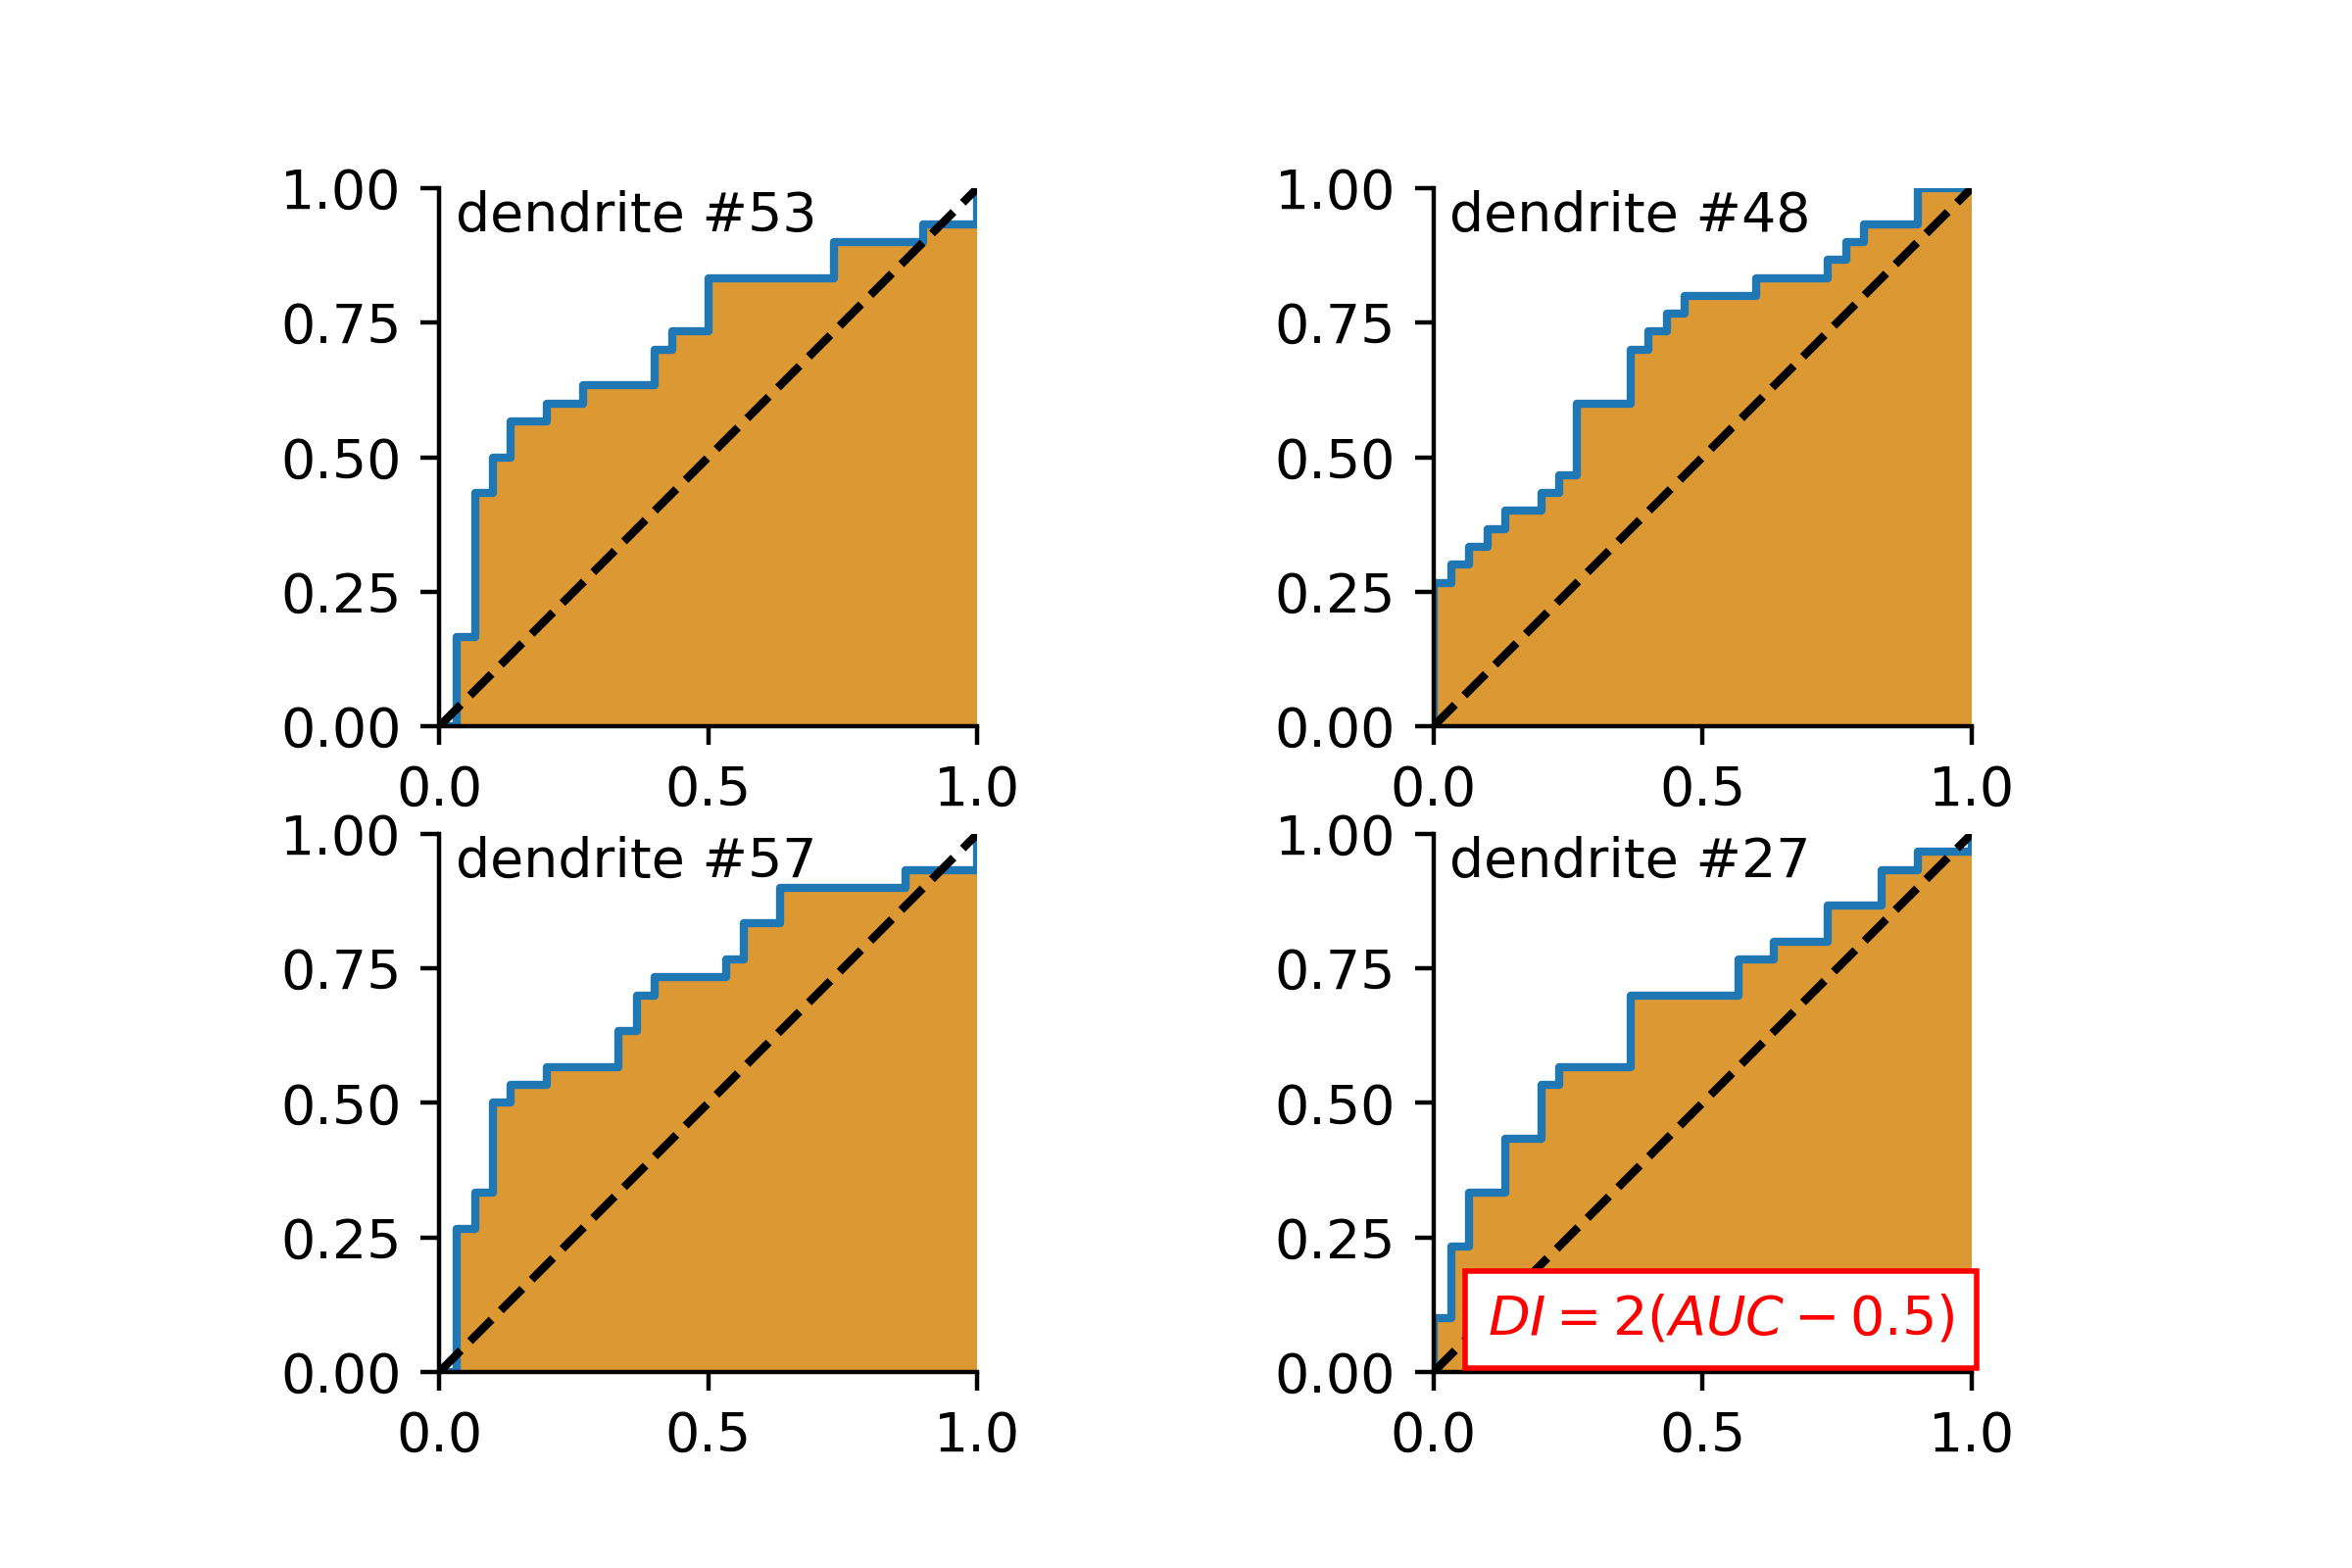
\includegraphics[width=1.0\textwidth]{roc_four.png}
	\end{figure}
	\end{center}
\end{frame}

%\begin{frame}[fragile]{Distribution of DI-Values}
%\begin{center}
%	\begin{figure}
%      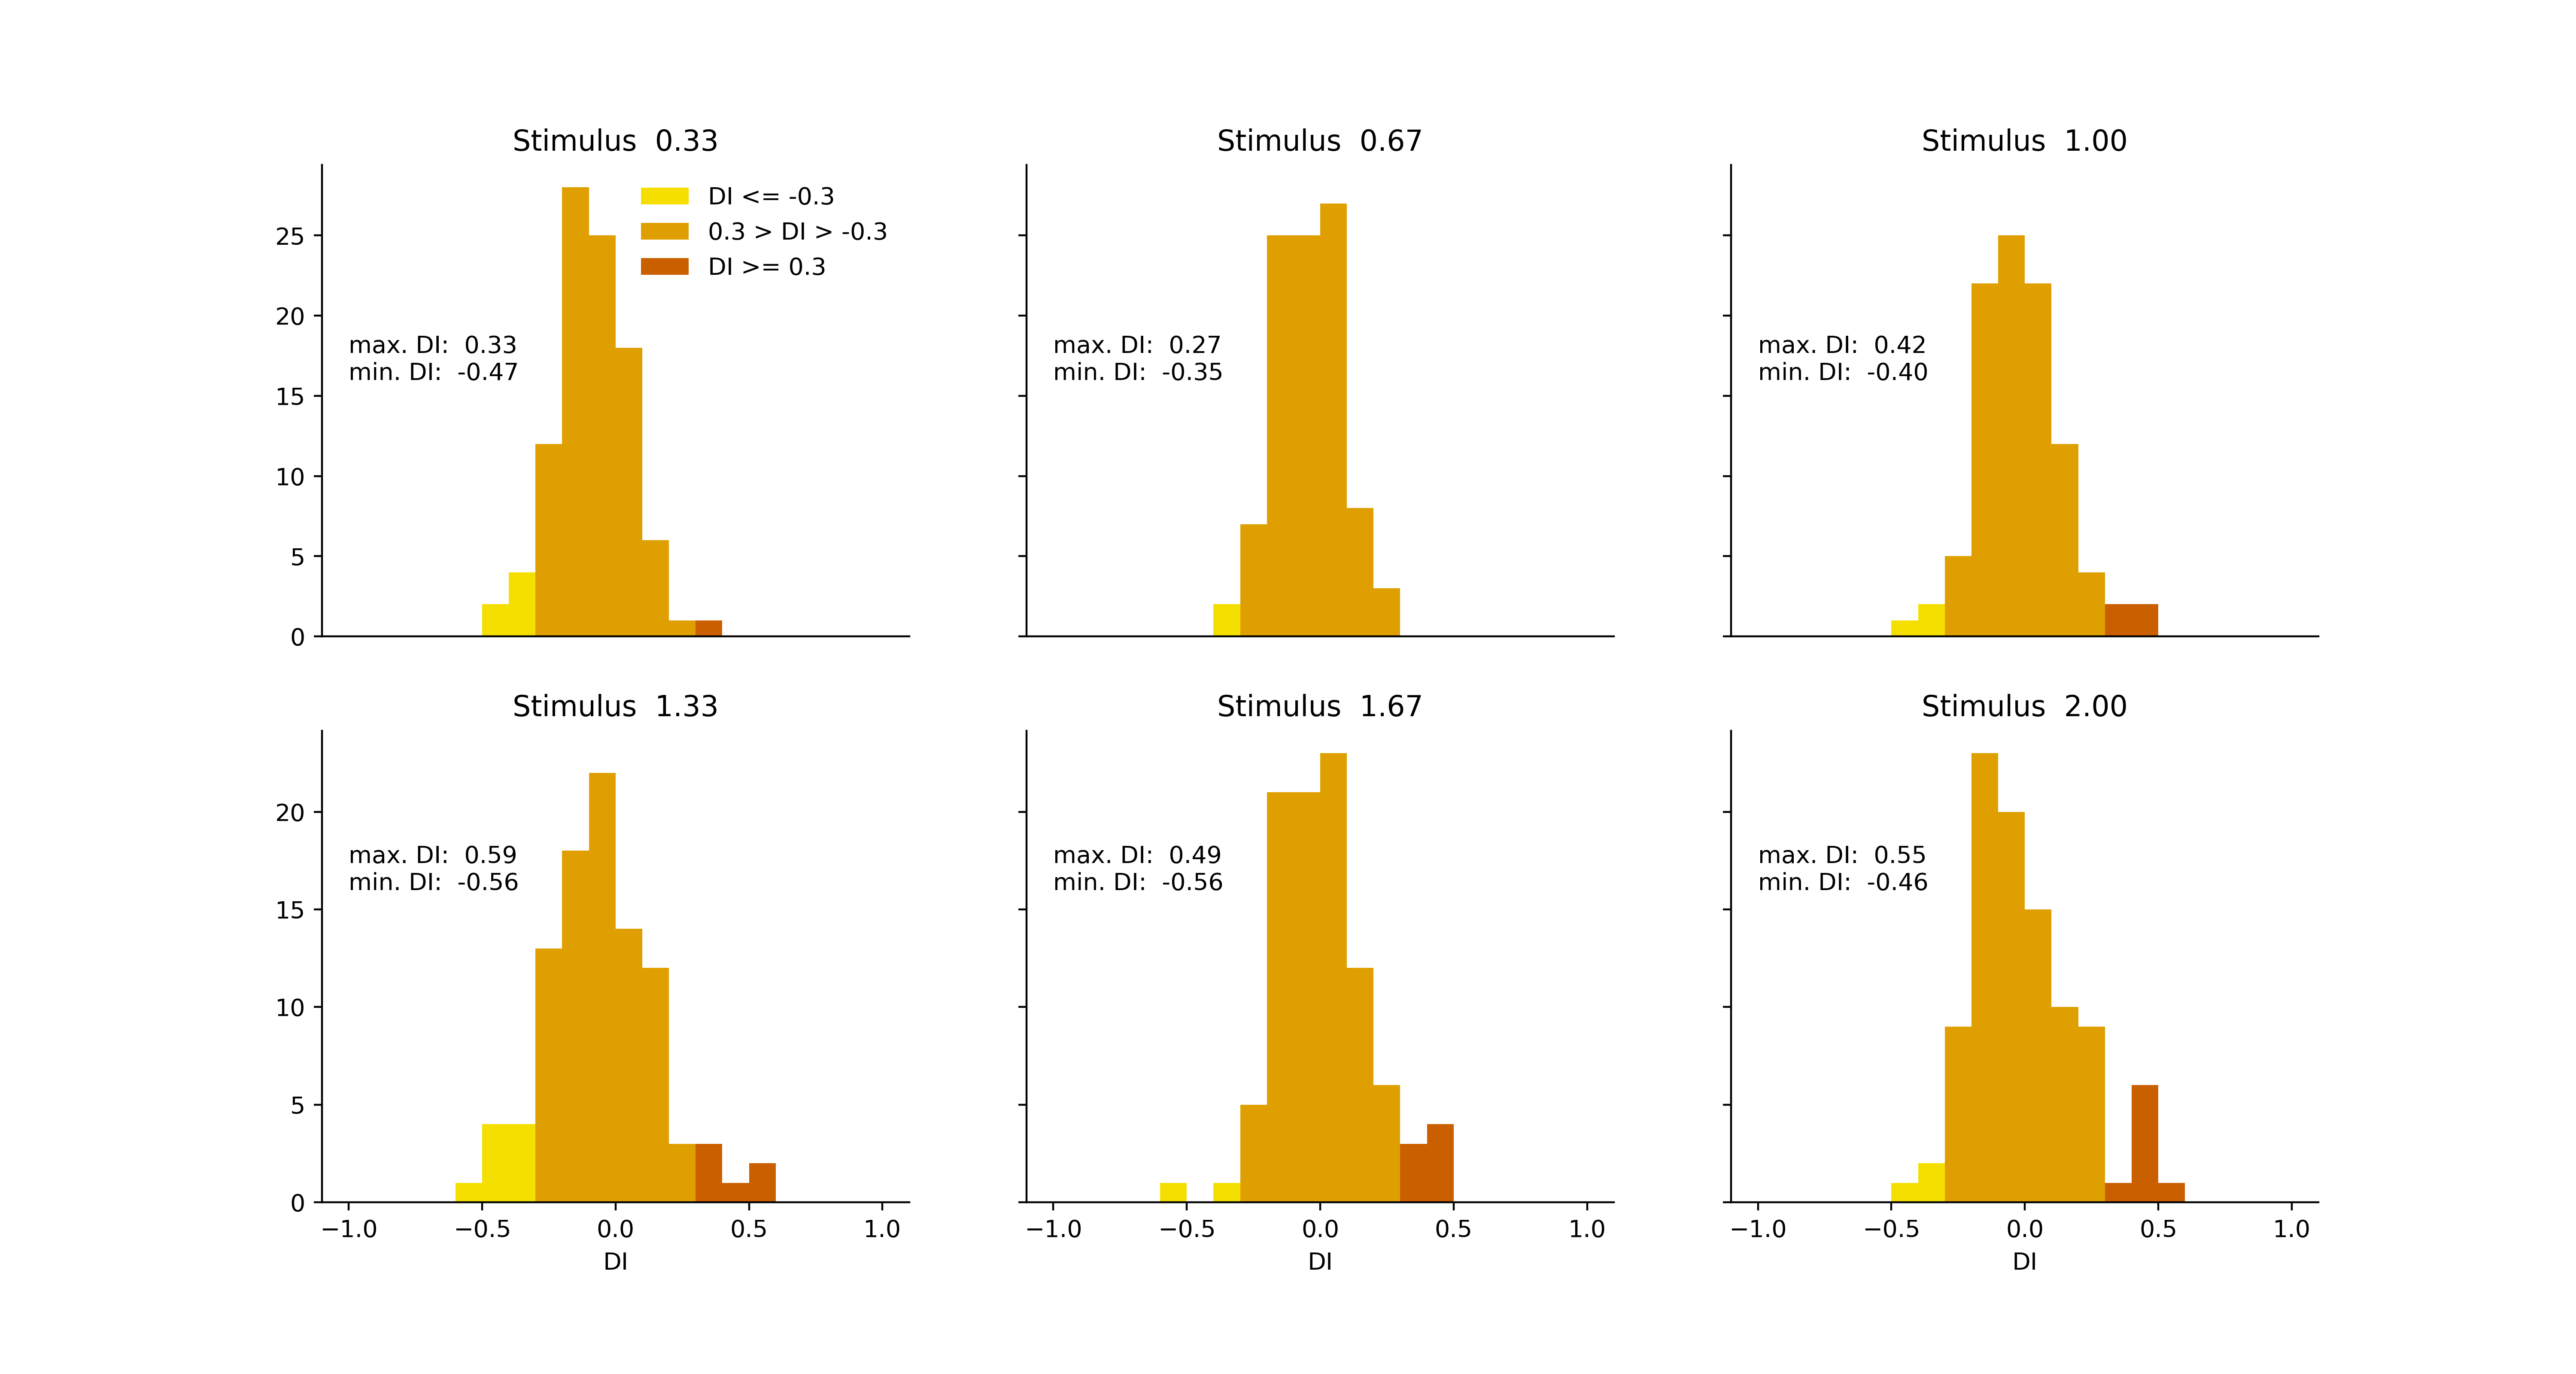
\includegraphics[width=1.0\textwidth]{DI_hist.png}
%	\end{figure}
%	\end{center}
%\end{frame}
%
%\begin{frame}[fragile]{Distribution of DI-Values vs. Chance}
%\begin{center}
%	\begin{figure}
%      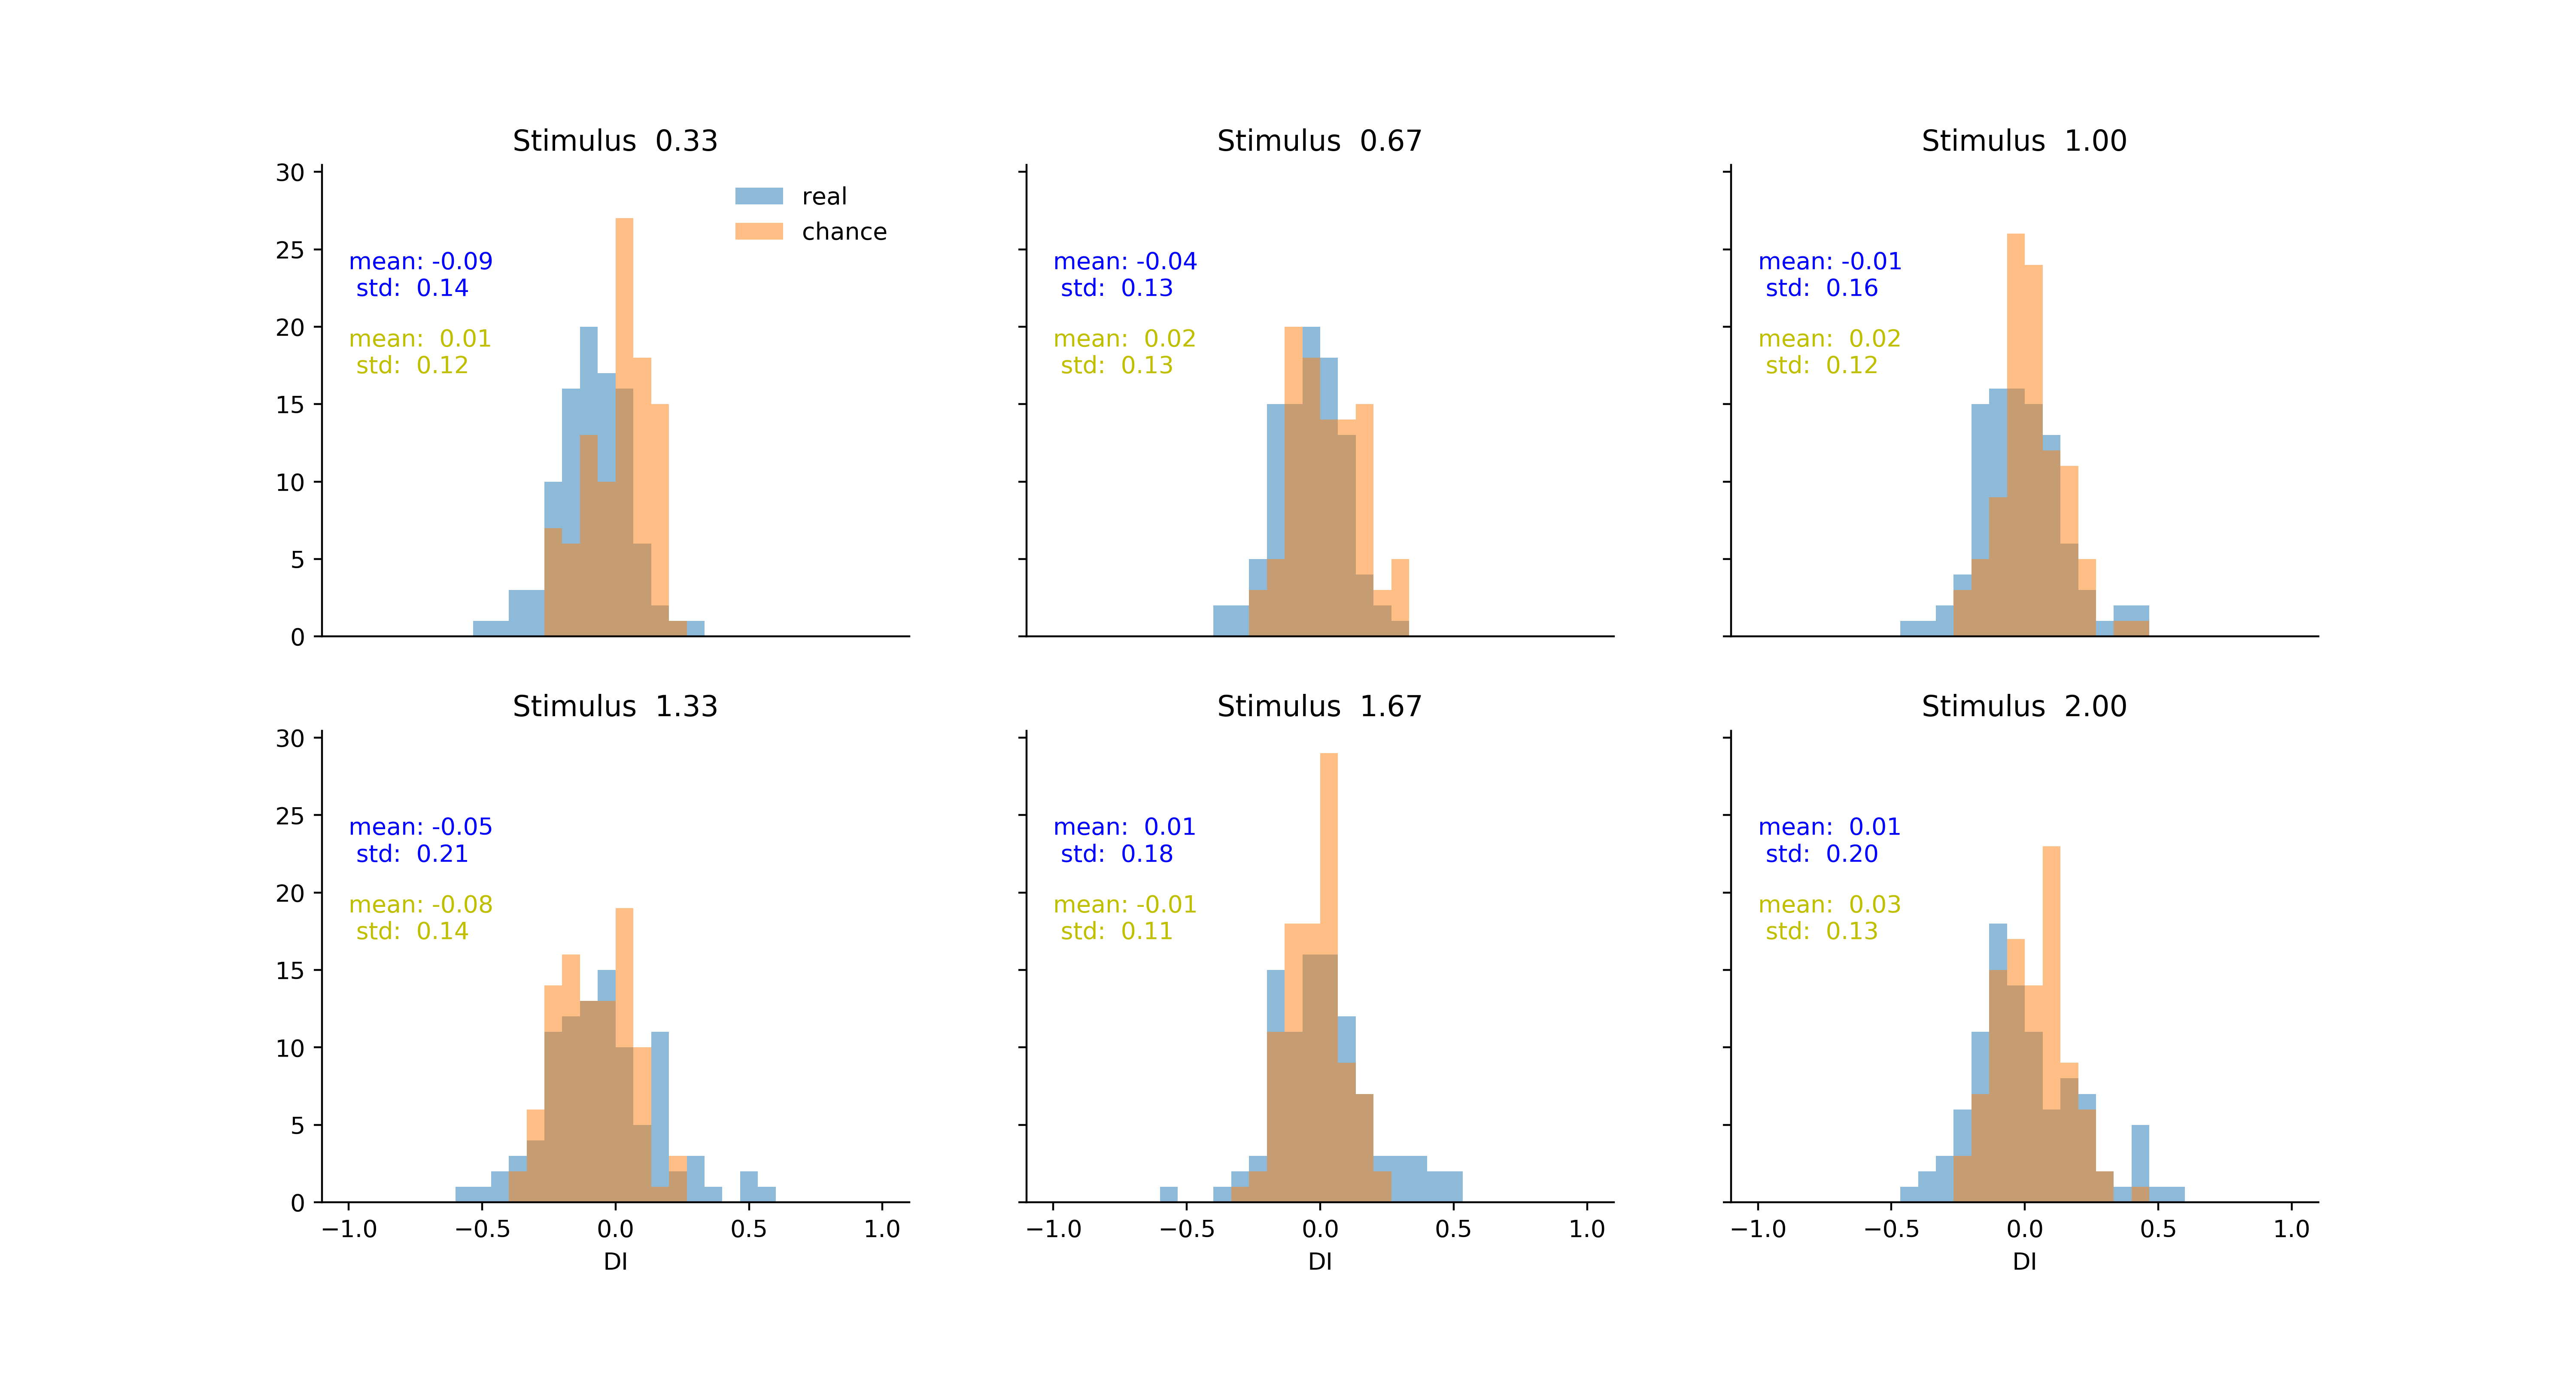
\includegraphics[width=1.0\textwidth]{realchance.png}
%	\end{figure}
%	\end{center}
%\end{frame}

\begin{frame}[fragile]{$\text{Ca}^{2+}$-Trace of Largest $|\text{DI}|$-Dendrites}
\begin{center}
	\begin{figure}
      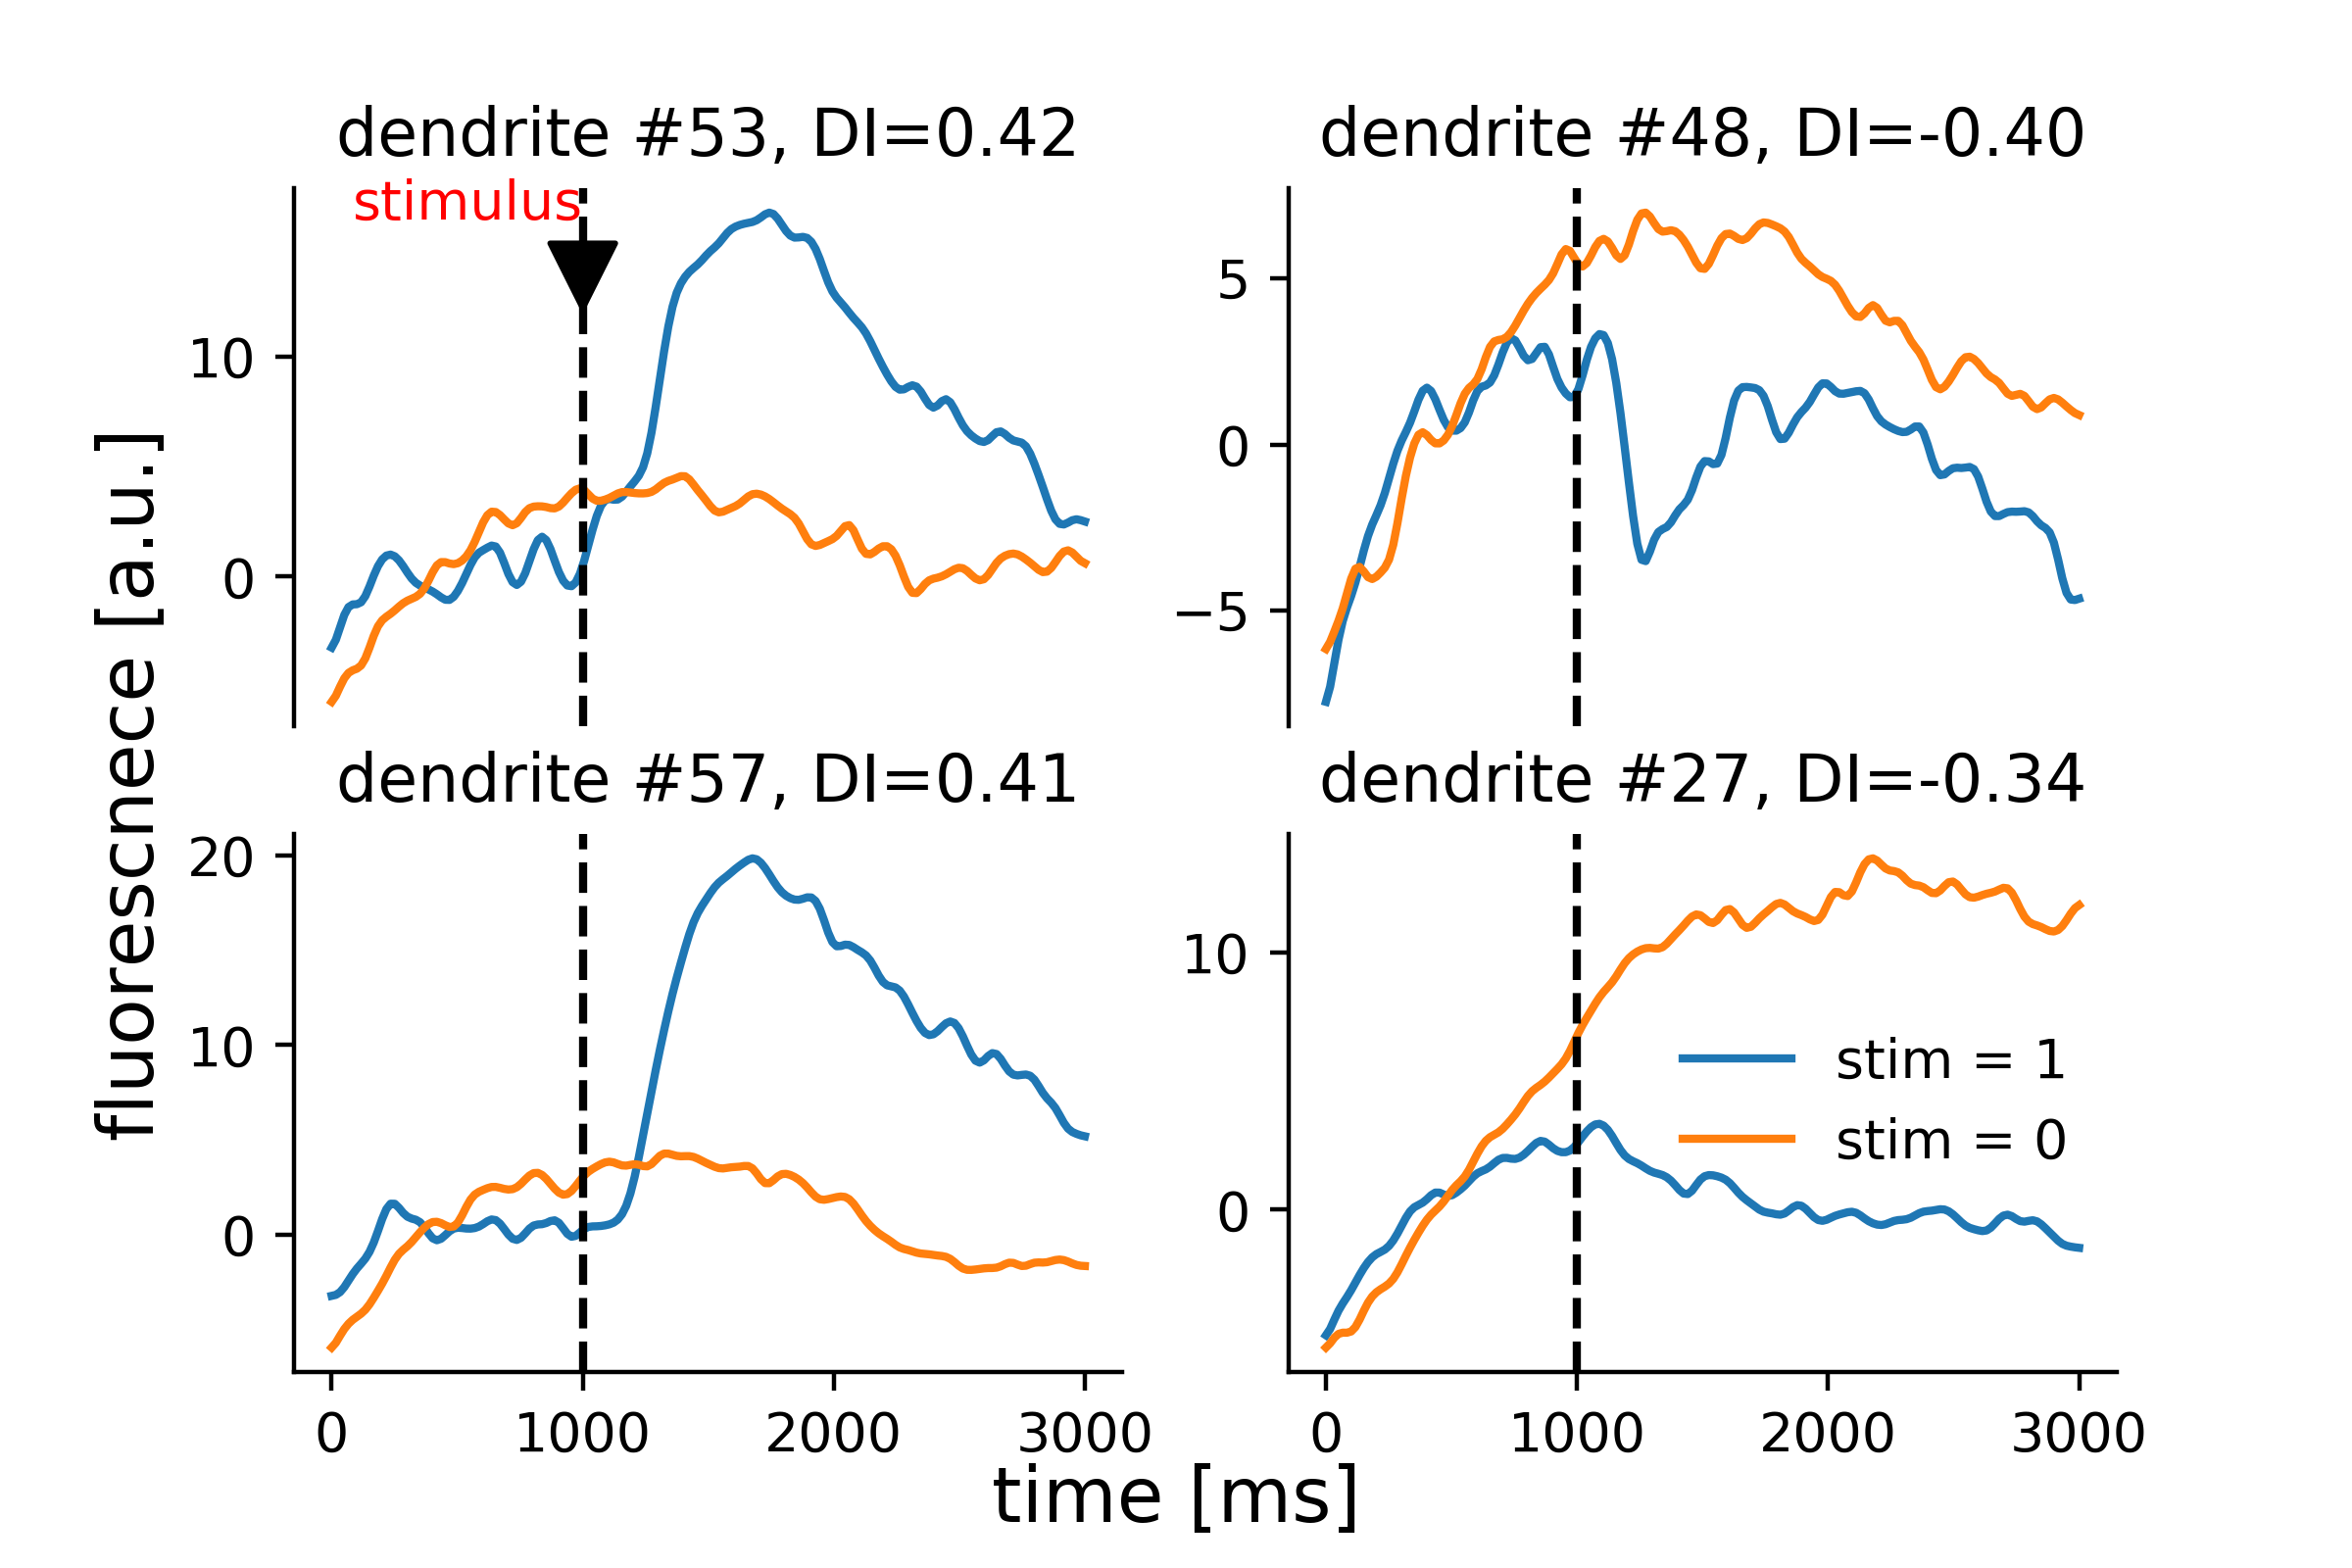
\includegraphics[width=1.0\textwidth]{on_vs_off.png}
      \caption*{Near threshold-stimulus ($\approx 1$)}
	\end{figure}
	\end{center}
\end{frame}

%\begin{frame}[fragile]{ROC Scores of Single Dendrites Using SVM}
%\begin{table}
%    \caption*{Stimulus strength 1 (near thereshold). Something is fishy here}
%    \begin{tabular}{c|c|c}
%      \toprule
%      Dendrite \# & Mean Accuracy & Standard Deviation\\
%      \midrule
%      57 & 0.44 & +/- 0.51\\
%      53 & 0.40 & +/- 0.28\\
%      48 & 0.38 & +/- 0.49\\
%      2 & 0.37 & +/- 0.74\\
%      \bottomrule
%    \end{tabular}
%  \end{table}
%\end{frame}

\begin{frame}[fragile]{SVM - What is an SMV?}
\begin{center}
\only<+->{
\begin{figure}
      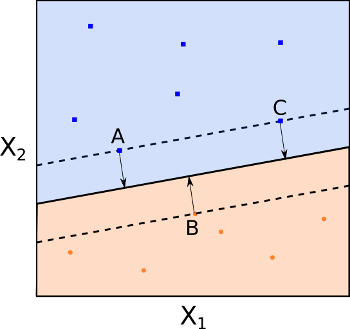
\includegraphics[height=0.3\textwidth]{svm_exp1.png}
	\end{figure}}
	\only<+->{
	\begin{figure}
      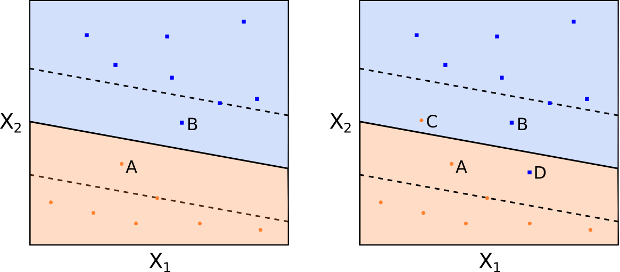
\includegraphics[height=0.3\textwidth]{svm_exp.png}
	\end{figure}}
	\end{center}
\end{frame}

\begin{frame}[fragile]{Why SVM?}

\begin{itemize}
\item staple of machine learning
\item regularization parameter limits overfitting
\item good for small samples with many features (in theory)
\end{itemize}

\end{frame}

\begin{frame}[fragile]{SVM Specifics}
\begin{itemize}
\item All data are normalized to zero mean and unit variance
\item Crossvalidation is performed to conrol for overfitting
\end{itemize}

\end{frame}

\begin{frame}[fragile]{SVM - Most Accurate Dendrites}
\begin{table}
    \caption*{Stimulus strength 1 (near thereshold)}
    \begin{tabular}{c|c|c}
      \toprule
      Dendrite \# & $\mu_{acc}$ & $\sigma_{acc}$\\
      \midrule
      57 & 0.70 & 0.12\\
      53 & 0.68 & 0.14\\
      48 & 0.63 & 0.13\\
      27 & 0.62 & 0.08\\
      \bottomrule
    \end{tabular}
  \end{table}
\end{frame}

\begin{frame}[fragile]{Rank Order Correlation}
\only<+->{
We want to quantify the similarity between two rank orders of dendrites $R$ and $Q$, which both have length $n$.}

\only<+->{
Standard approach: Spearman's rank order coefficient 
$$
\rho(R,Q) = 1 - \frac{6\sum_i^nD_i^2}{n(n	^2-1)}
$$
where $D_i=R_i-Q_i$.}

\only<+->{
Problem: Many of the dendrites are not significant for classification but affect $\rho$ greatly. We would like to be able to \textbf{weight our} $\mathbf{D_i}$'s.}
\end{frame}

\begin{frame}{Weighted Rank Order Correlation Coefficient}
One possible soulution:
$$
\rho_W(R,Q) = 1-\frac{-2\sum_i^nw_iD_i^2}{\sum_i^nw_i(n-2i+1)^2}
$$
With a monotonicity constraint on $W$.
\end{frame}

\begin{frame}[fragile]{Rank Order Correlations of Dendrites Over Stimuli}
\begin{center}
	\begin{figure}\caption*{Weighted rank coefficient $\rho_{\omega}$ (todo: find more optimal weights)}
      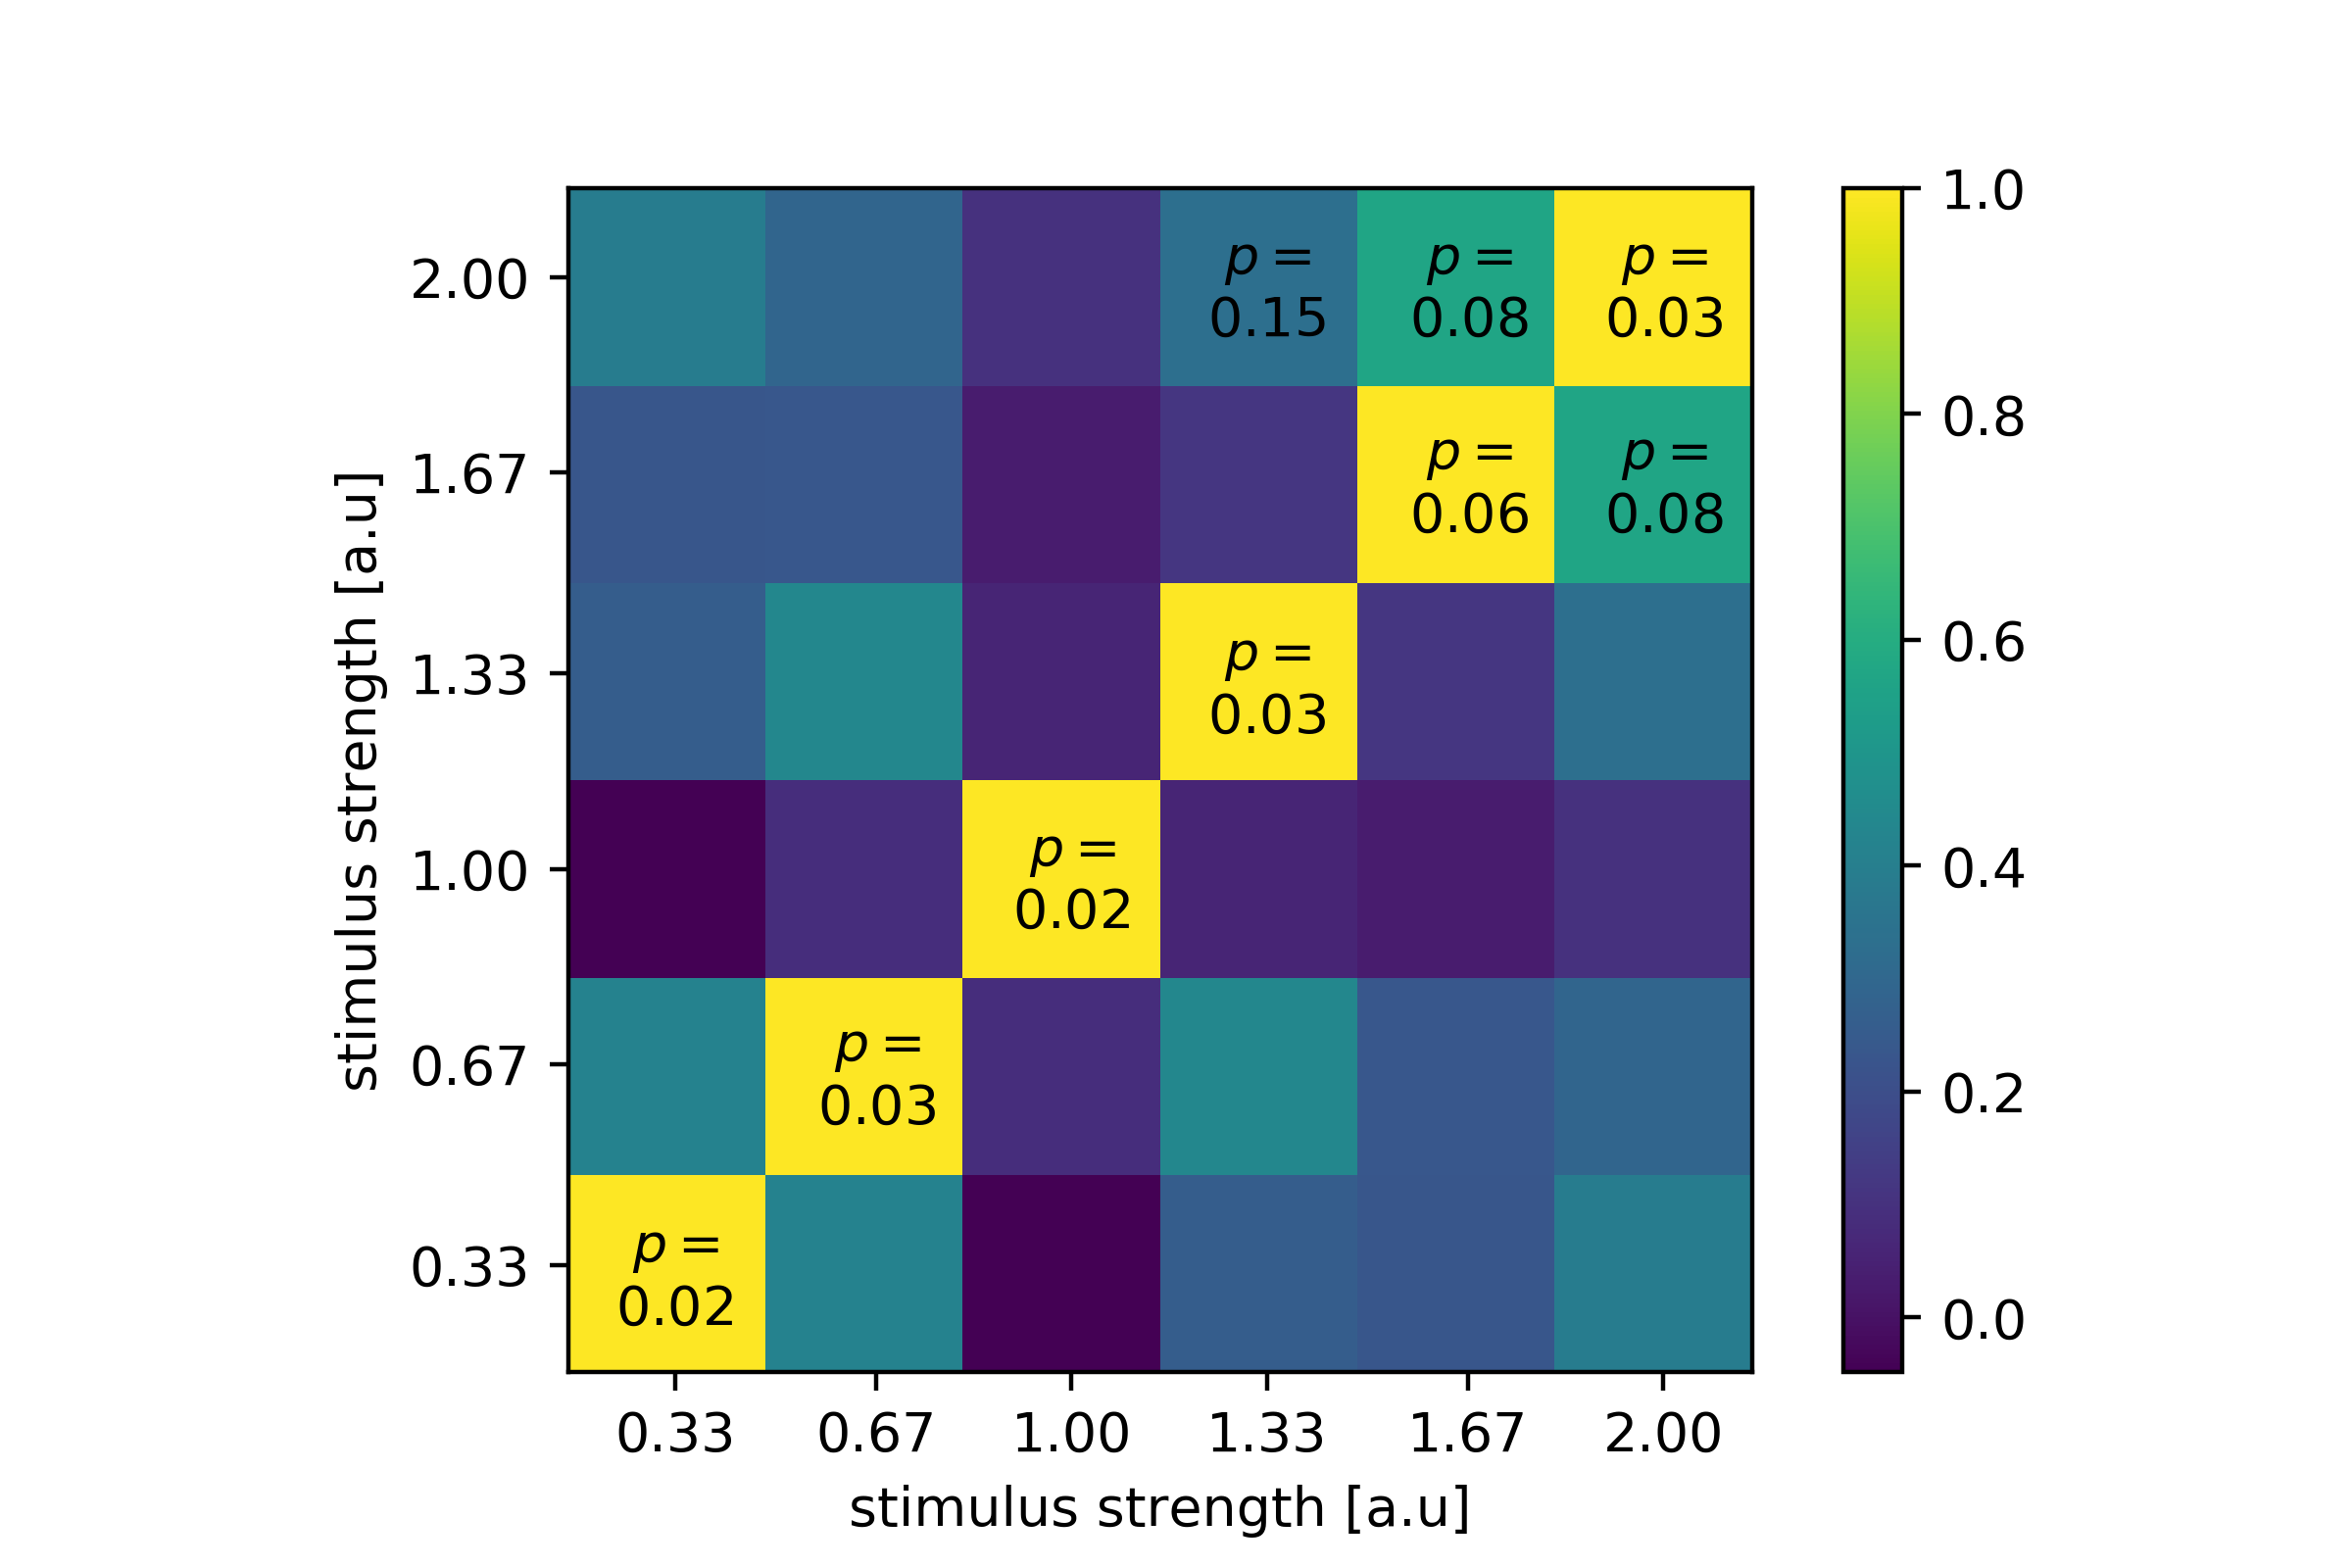
\includegraphics[width=1.0\textwidth]{rank_presence.png}
	\end{figure}
	\end{center}
\end{frame}

\begin{frame}[fragile]{Tuning Curves}
\begin{center}
	\begin{figure}
      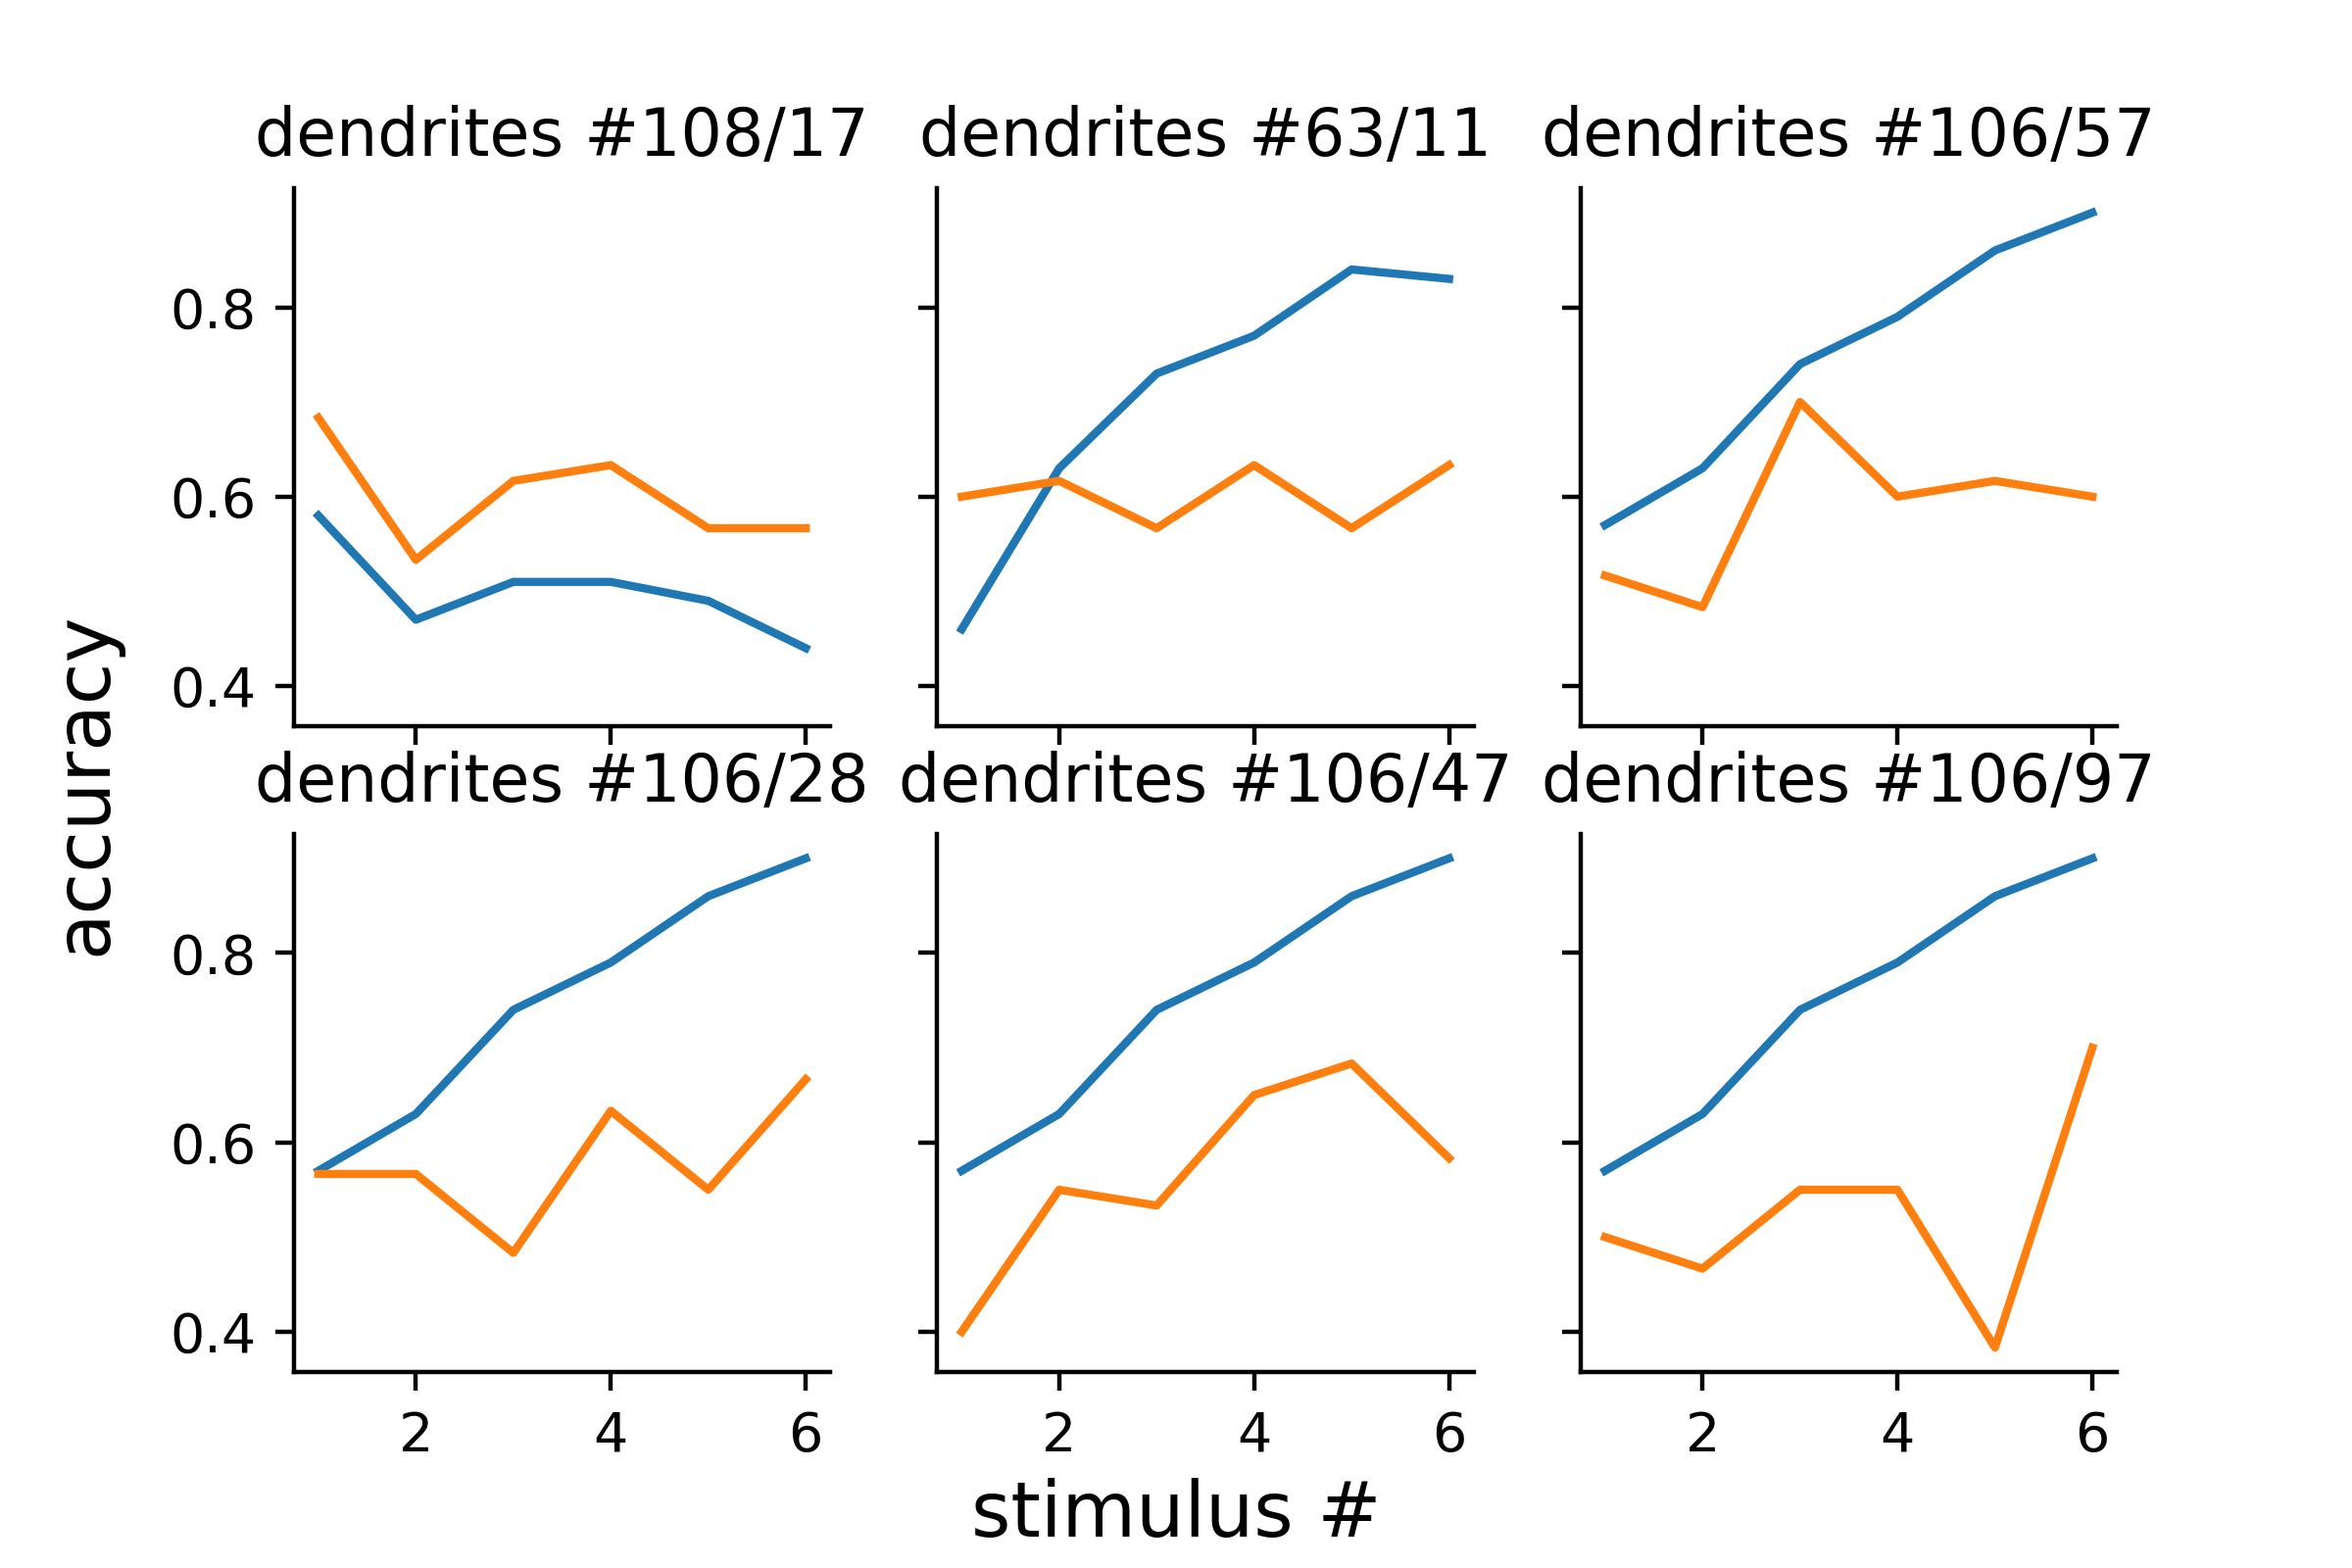
\includegraphics[width=1.0\textwidth]{tuning.png}
	\end{figure}
	\end{center}
\end{frame}

\begin{frame}[fragile]{Tuning Curves}
\begin{center}
	\begin{figure}
      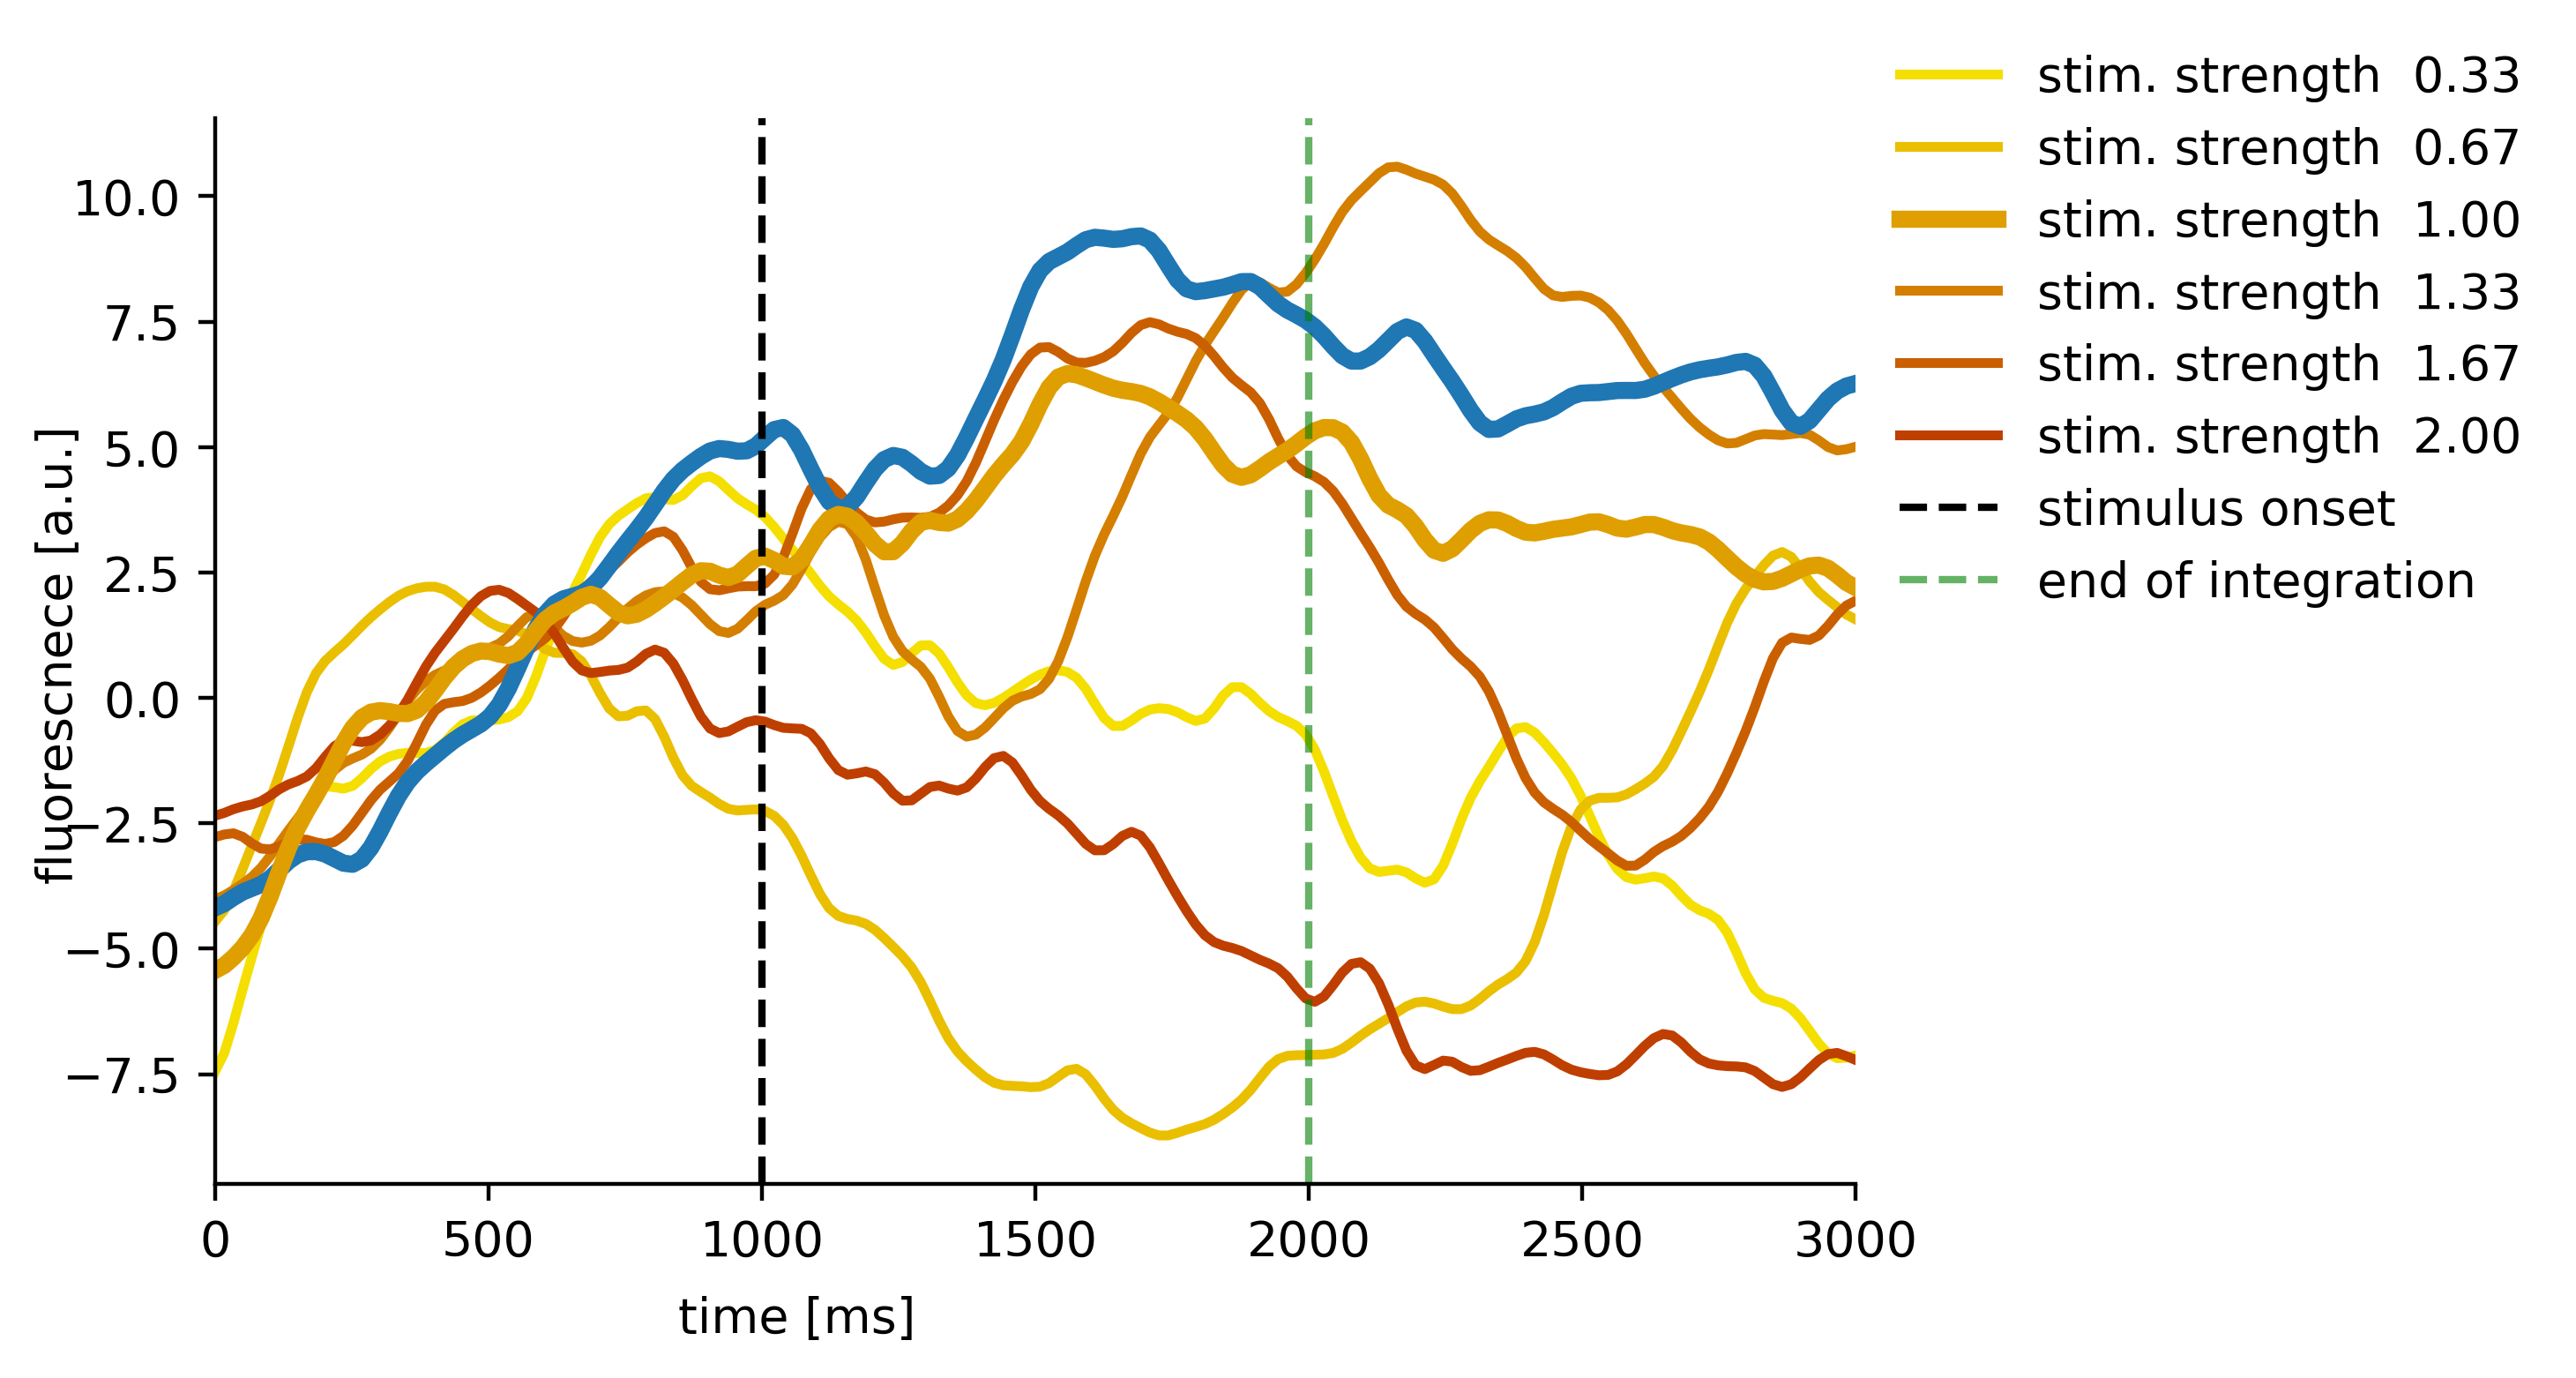
\includegraphics[width=1.0\textwidth]{tuning_ca2+single.png}
	\end{figure}
	\end{center}
\end{frame}

\begin{frame}[fragile]{Tuning Curves}
\begin{center}
	\begin{figure}
      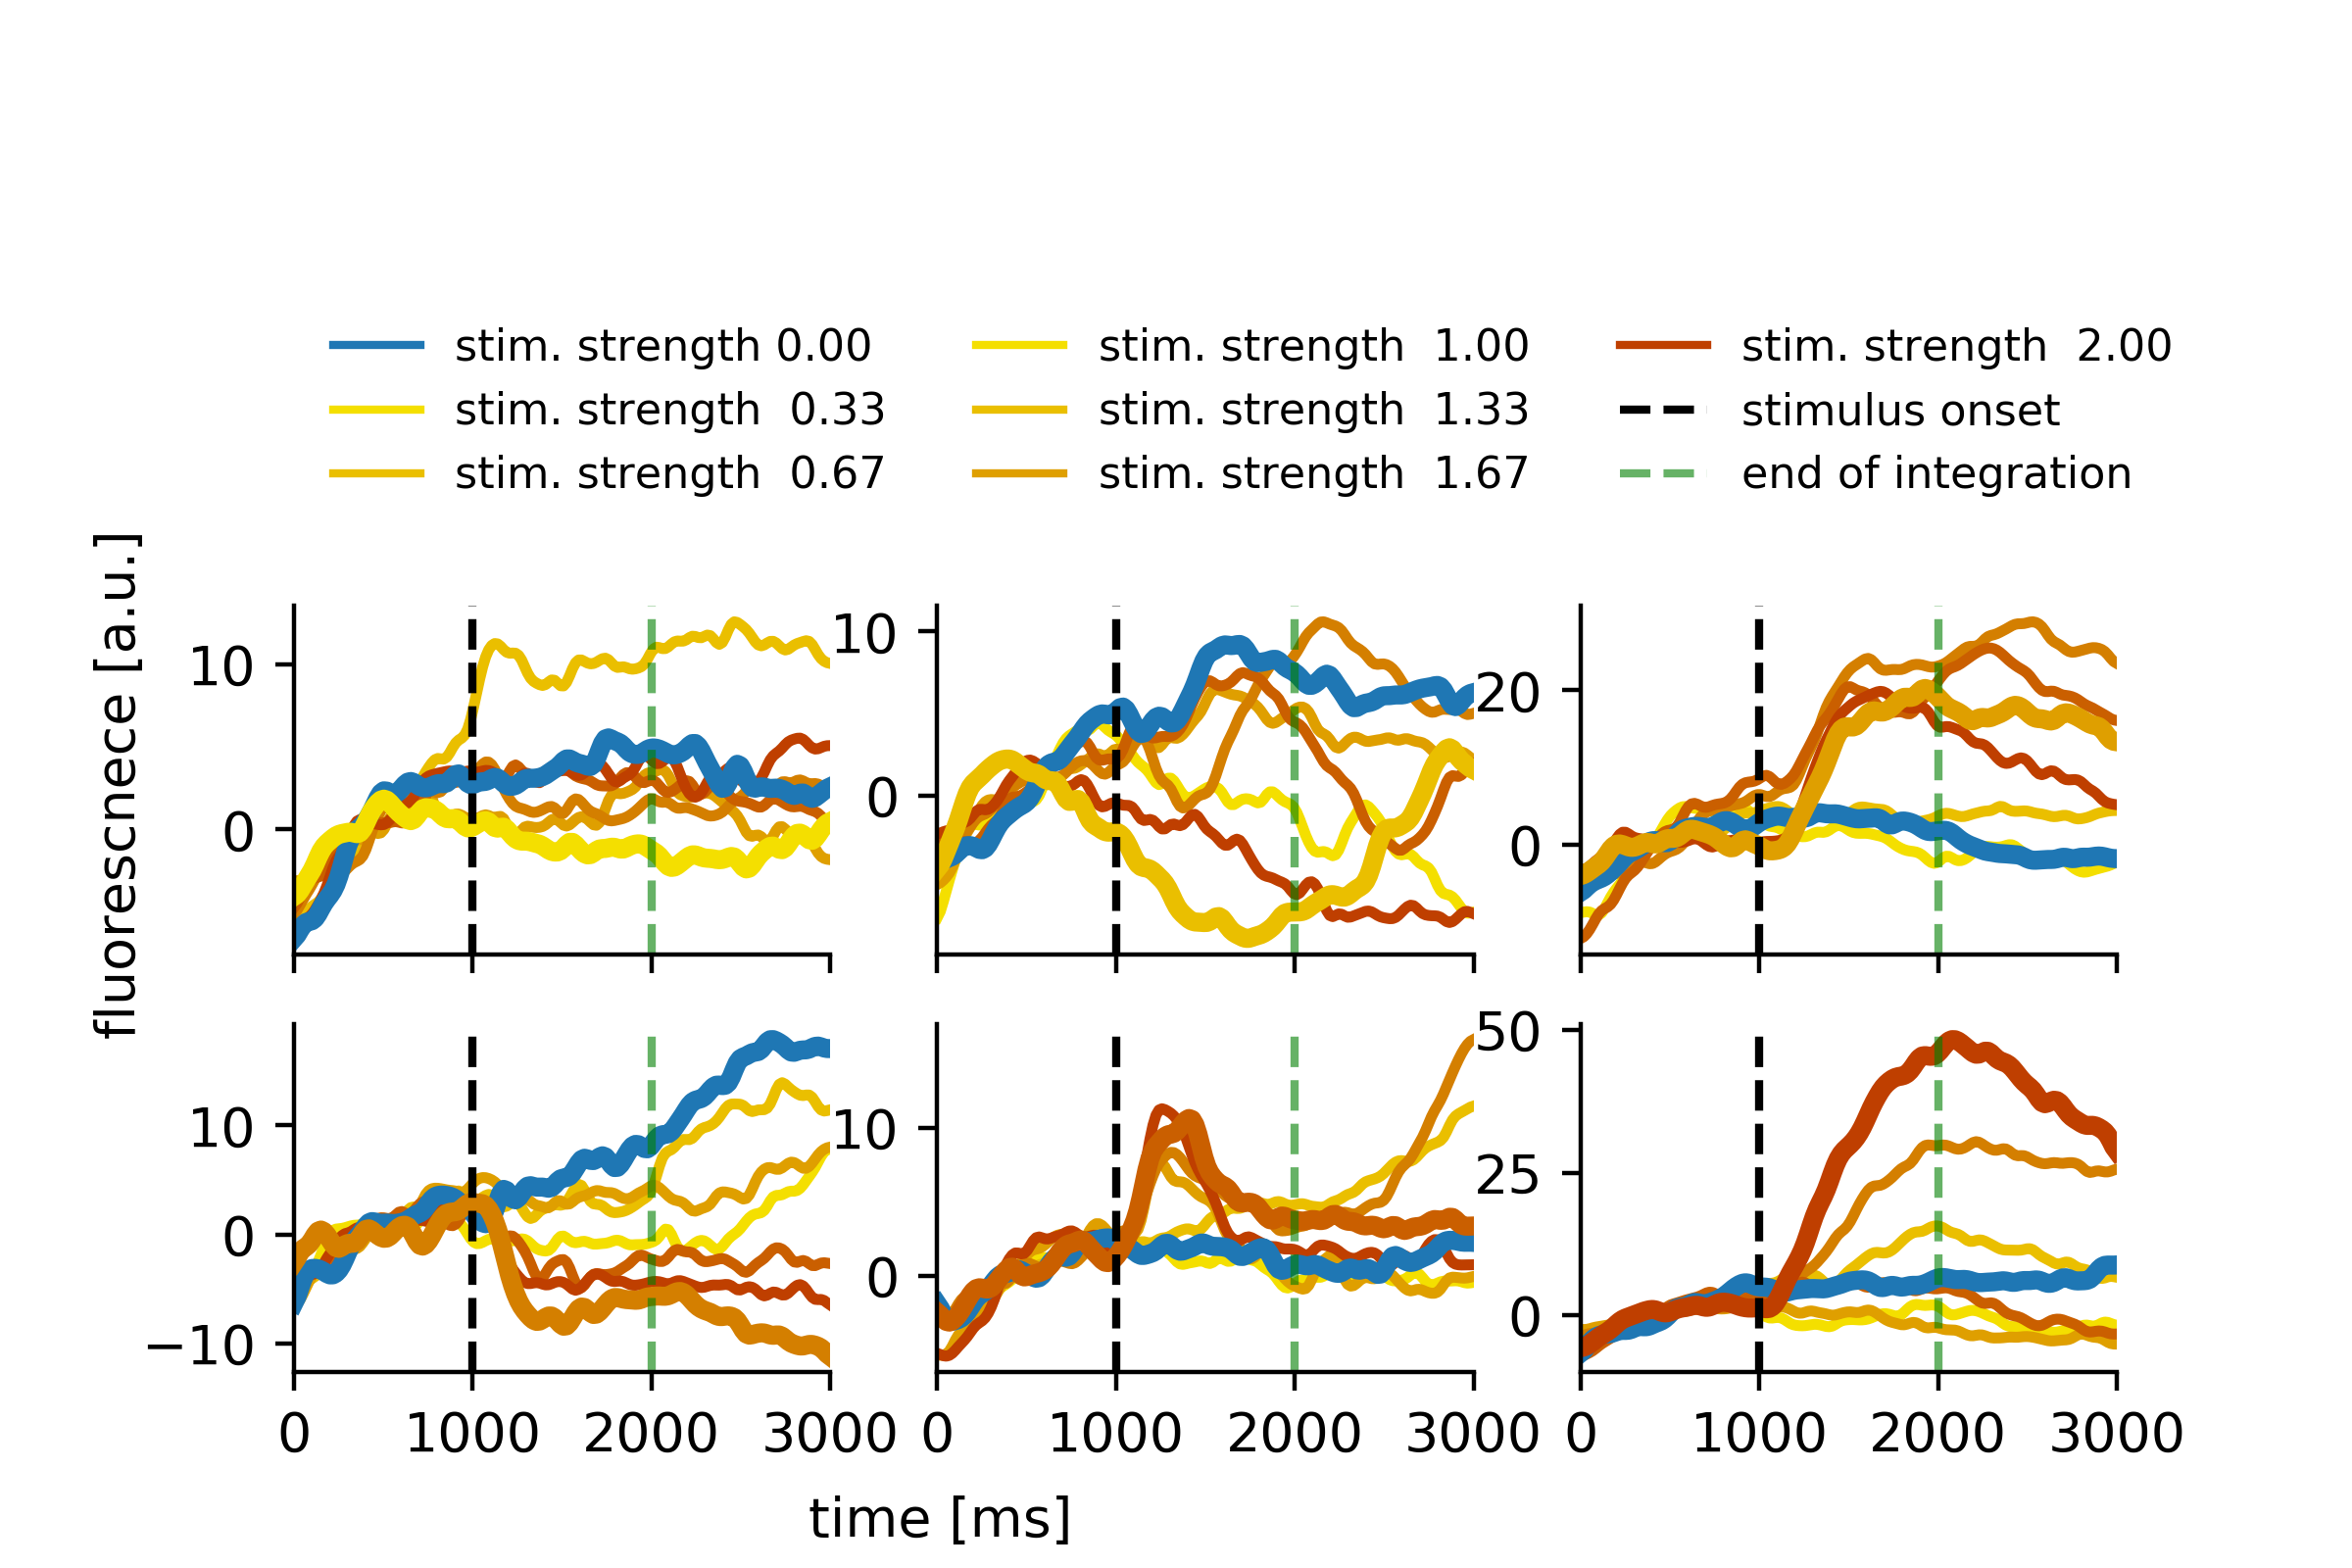
\includegraphics[width=1.0\textwidth]{tuning_ca2+.png}
	\end{figure}
	\end{center}
\end{frame}

\begin{frame}[fragile]{Bevahior Detection}
\begin{center}
	\begin{figure}
      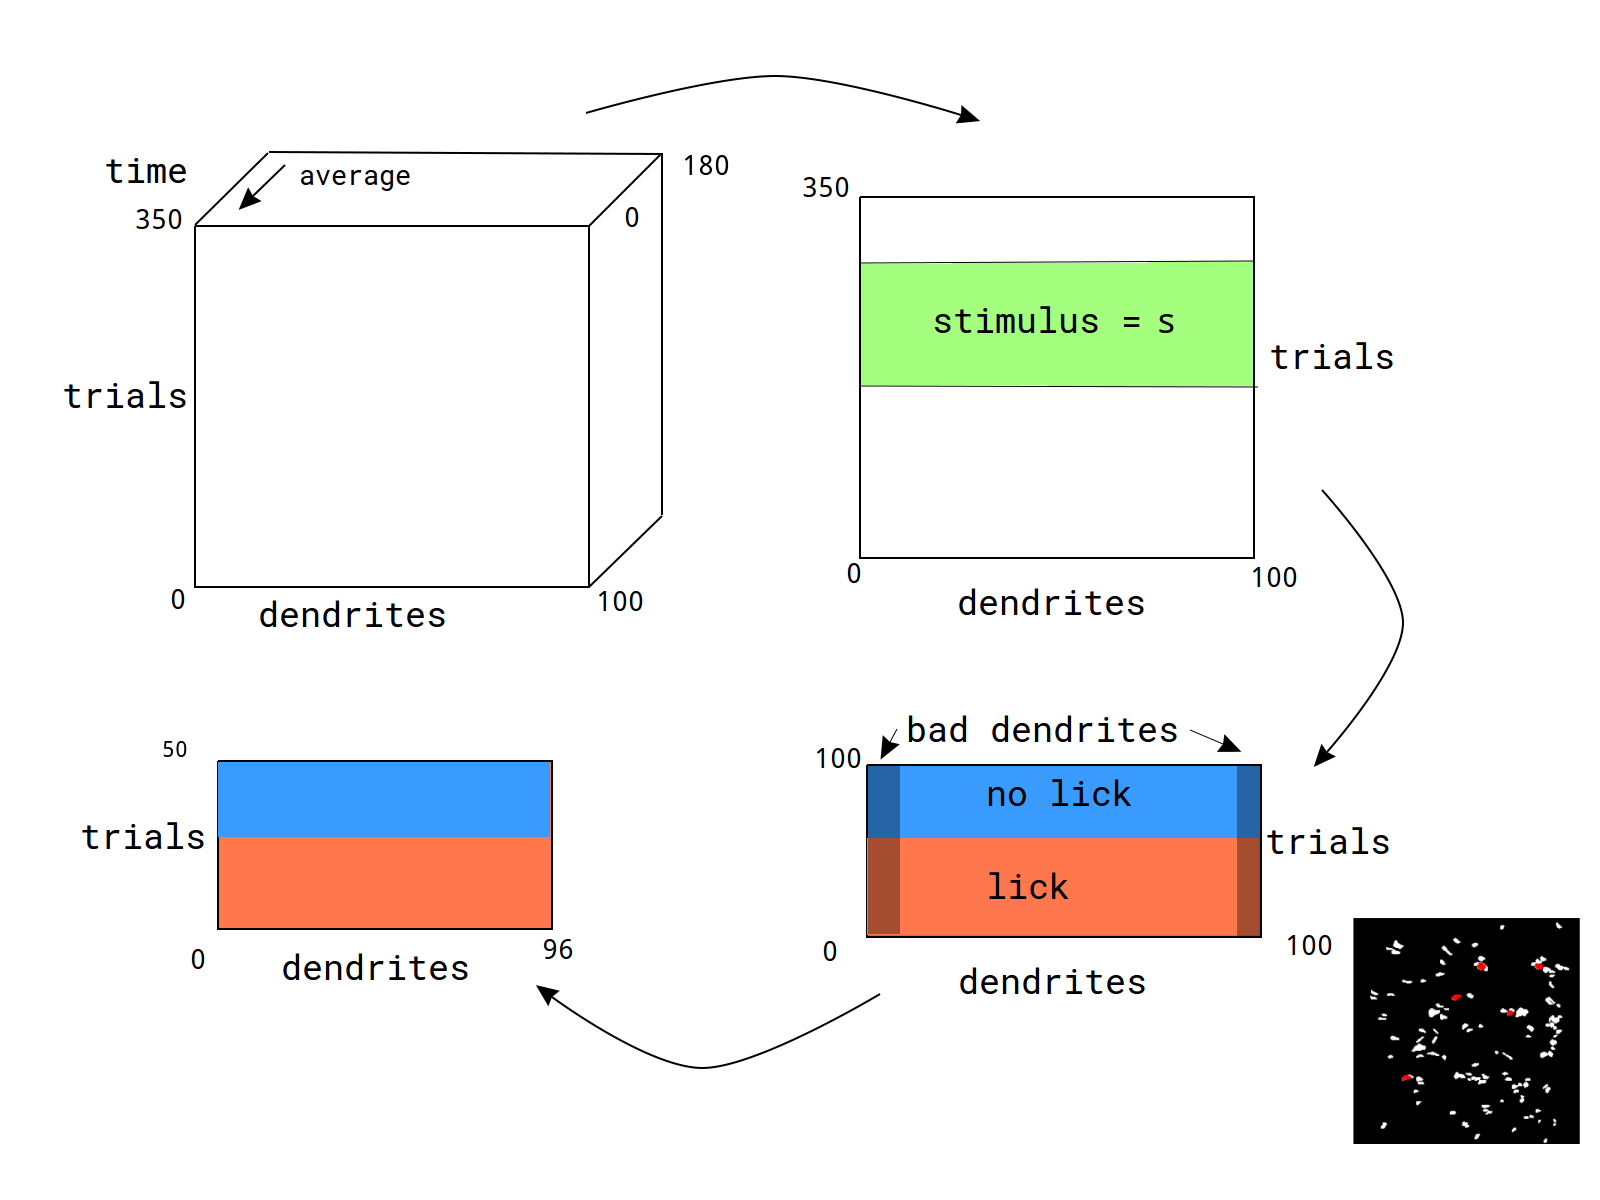
\includegraphics[width=1.0\textwidth]{data_hm.png}
	\end{figure}
	\end{center}
\end{frame}

\begin{frame}[fragile]{Behavioral Prediction - Most Accurate Dendrites}
\begin{table}
    \caption*{Different dataset - Stimulus strength 1 (near thereshold)}
    \begin{tabular}{c|c|c}
      \toprule
      Dendrite \# & $\mu_{acc}$ & $\sigma_{acc}$\\
      \midrule
      88 & 0.80 & 0.08\\
      57 & 0.80 & 0.08\\
      92 & 0.78 & 0.06\\
      56 & 0.76 & 0.10\\
      \bottomrule
    \end{tabular}
  \end{table}
\end{frame}

\begin{frame}[fragile]{Behavorial Predition - Imbalance}
\begin{center}
	\begin{figure}
	  \caption*{$N_{no-lick}$ vs. $N_{lick}$ for all stimuli}
      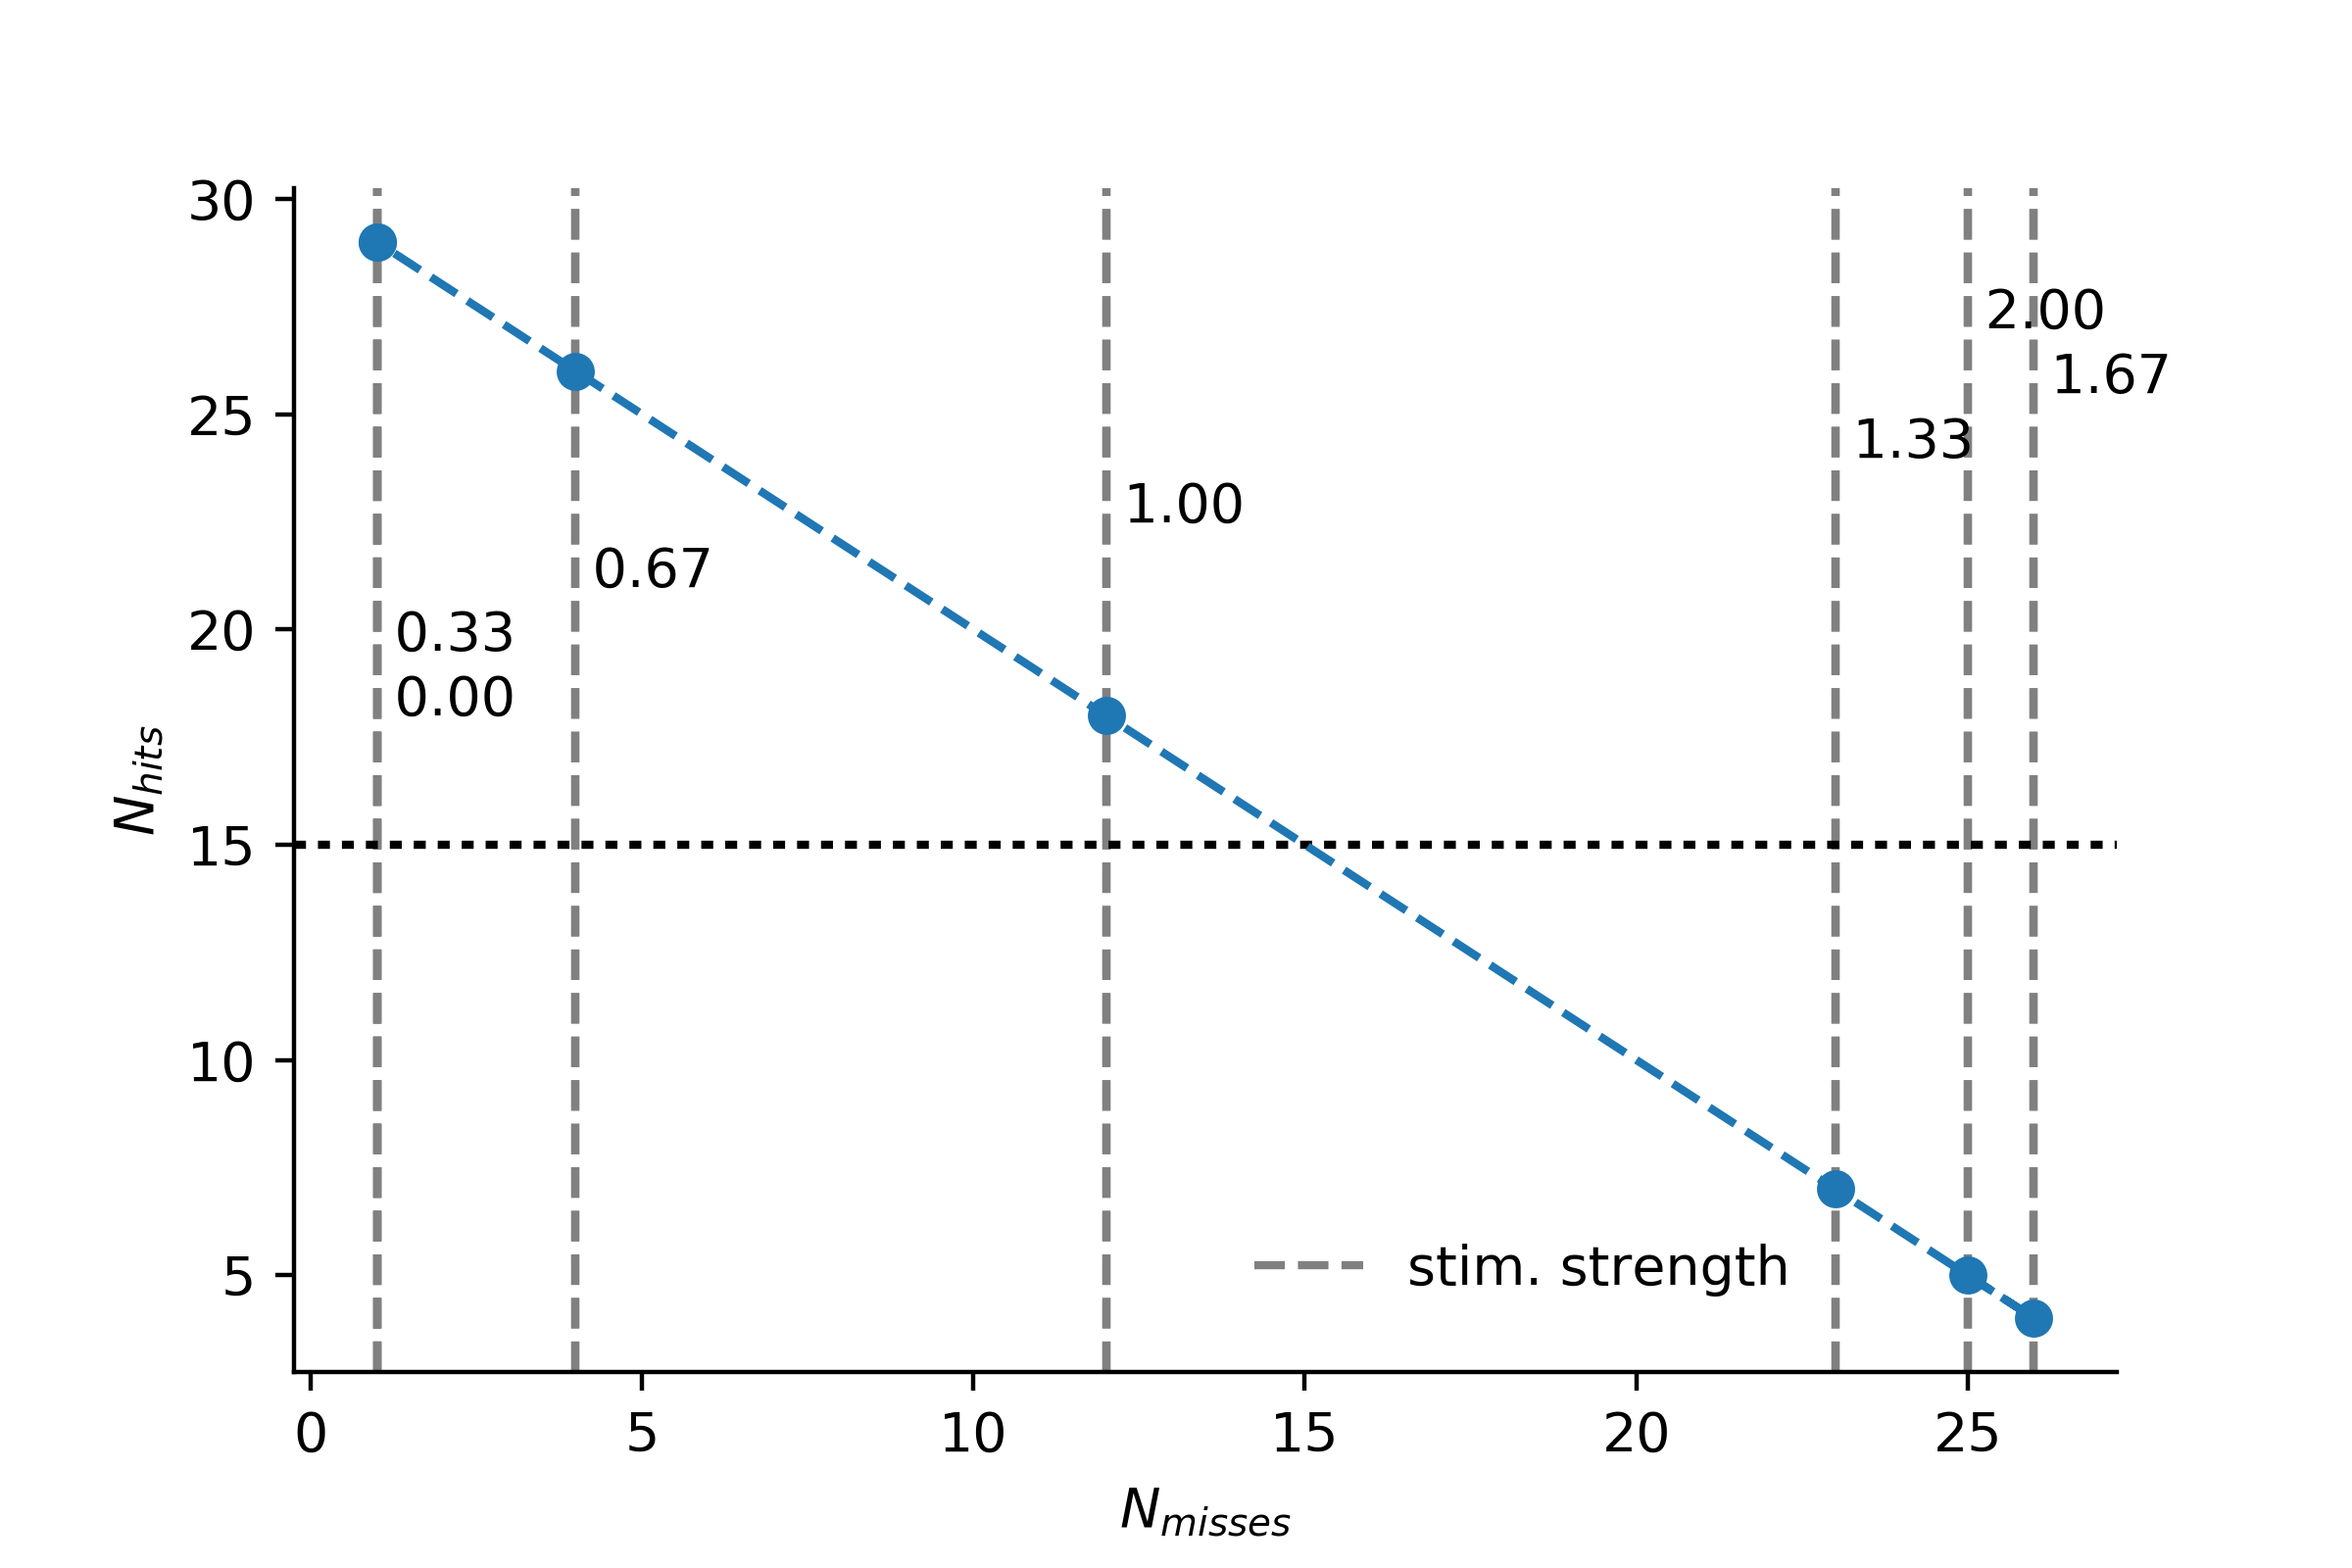
\includegraphics[width=1.0\textwidth]{fraction.png}
	\end{figure}
	\end{center}
\end{frame}

%\begin{frame}[fragile]{Behavoreal Tuning}
%\begin{center}
%	\begin{figure}
%      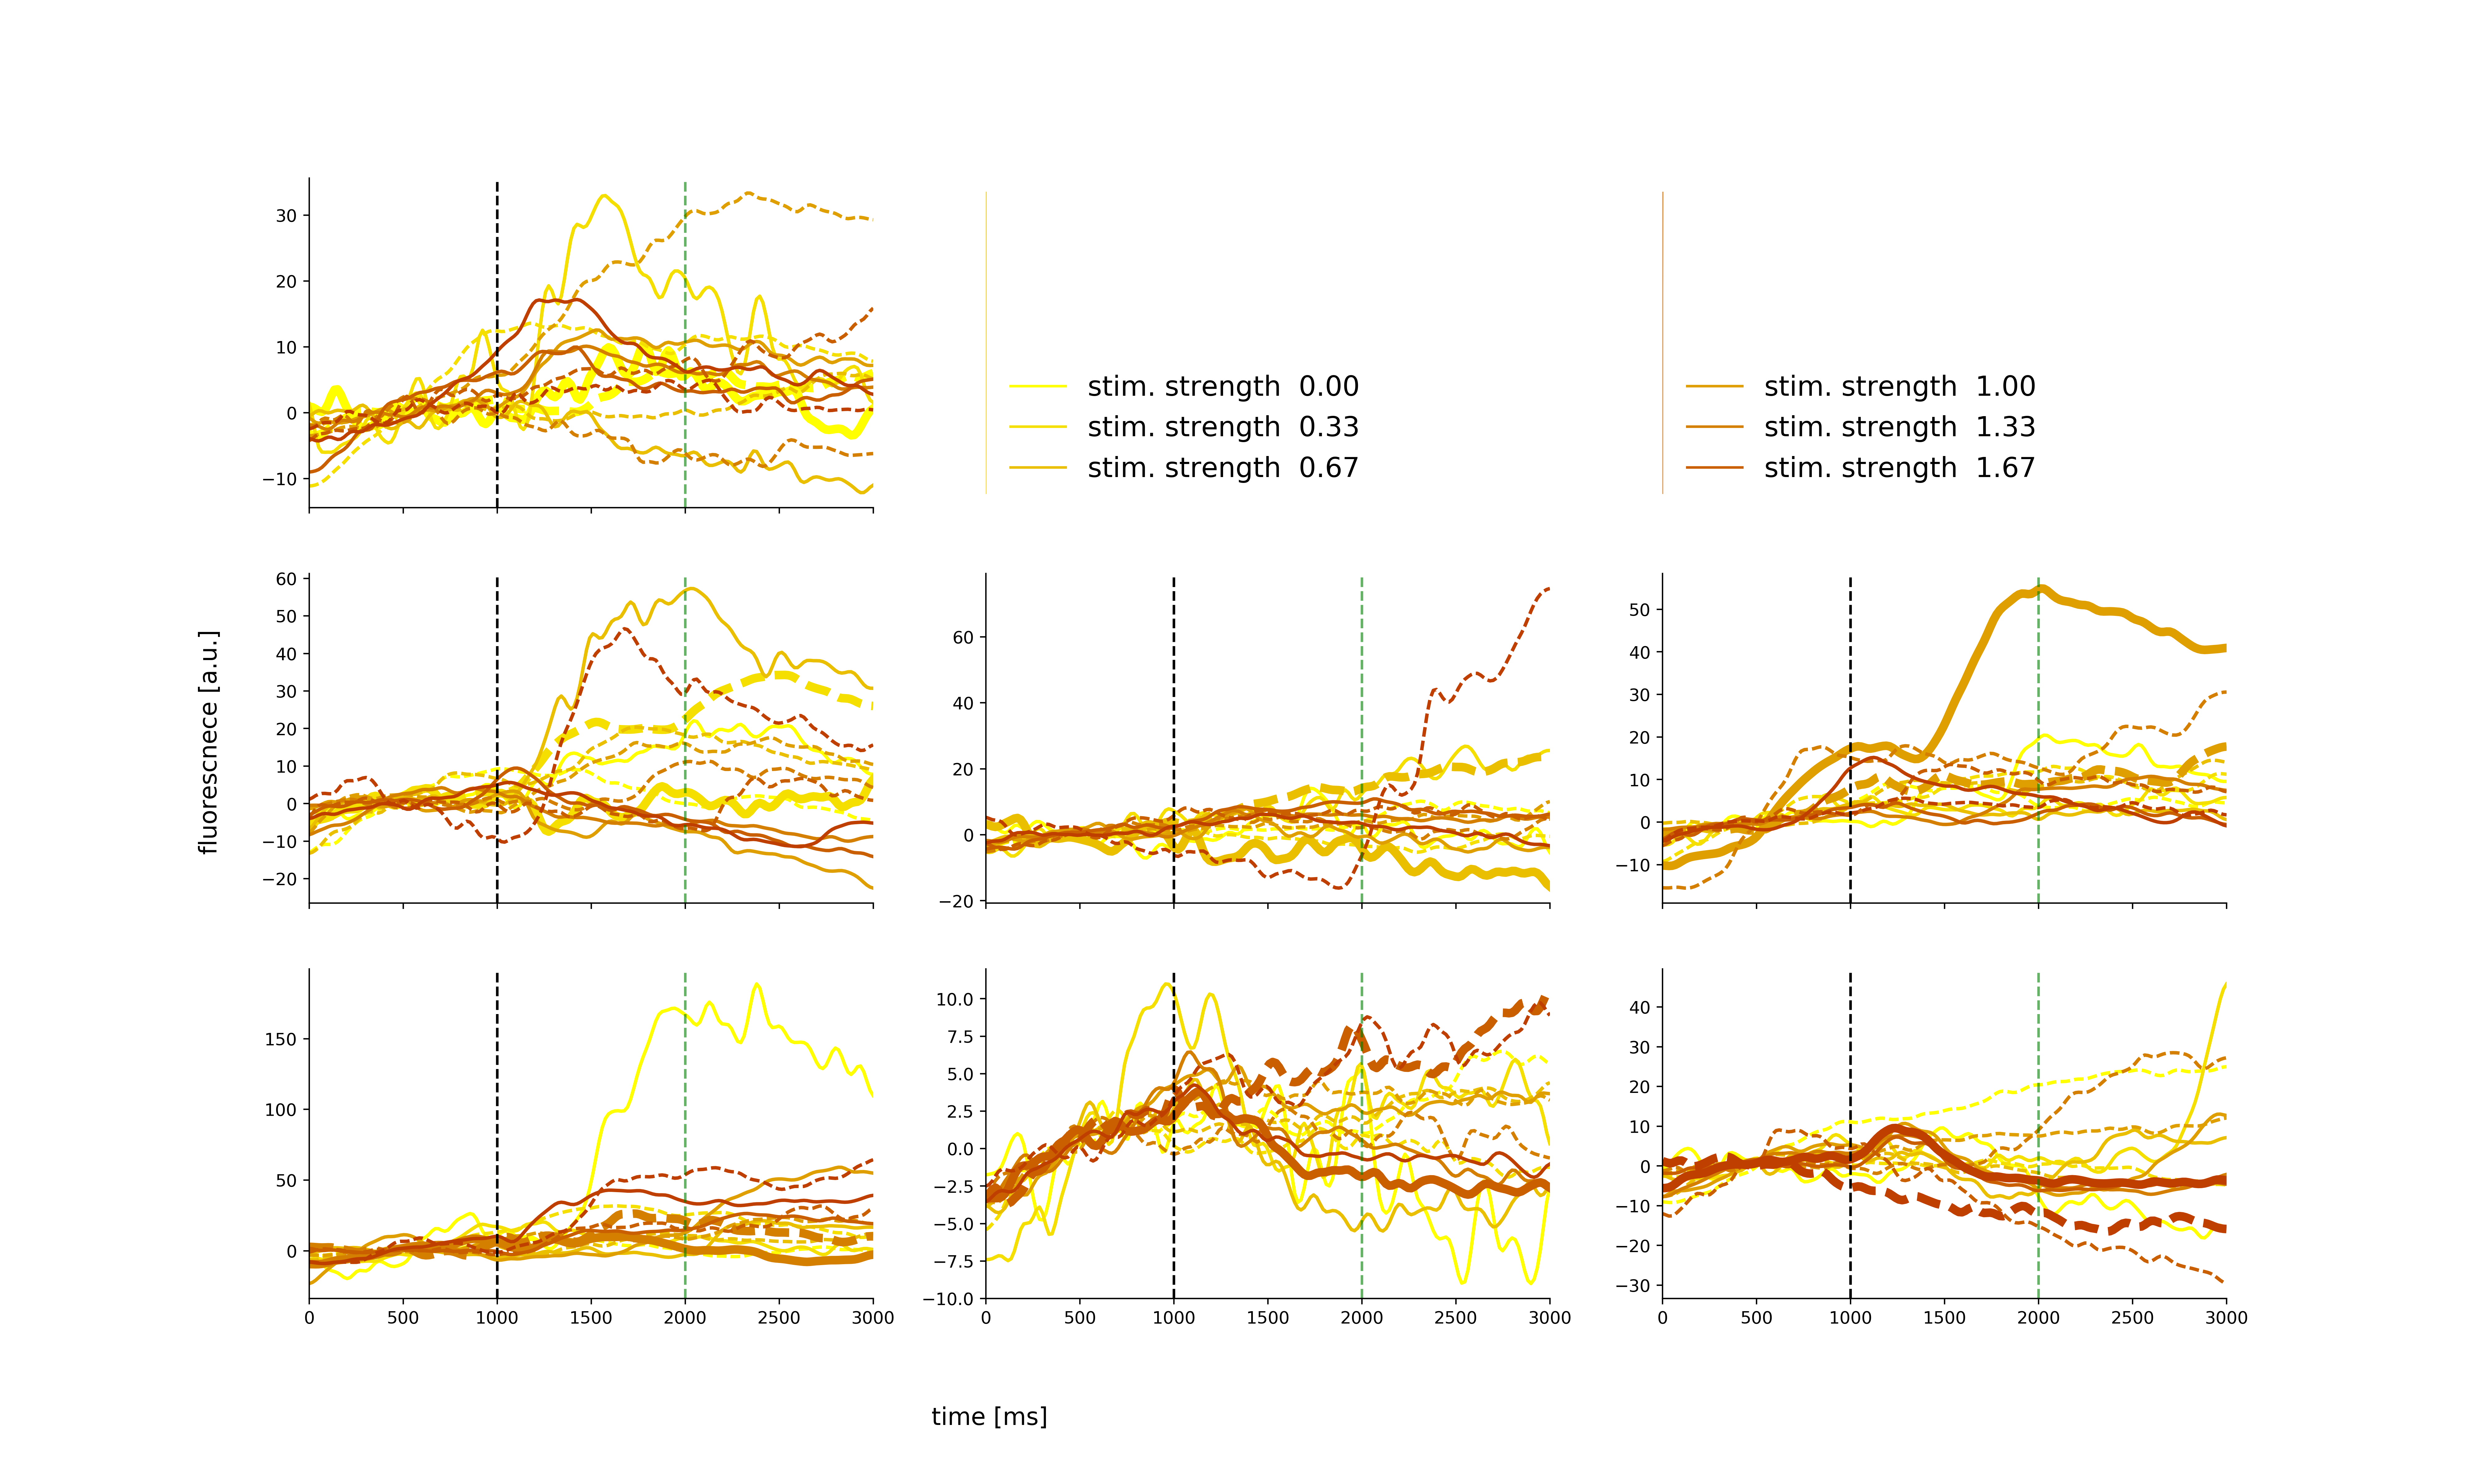
\includegraphics[width=1.0\textwidth]{tuning_ca2+_bb.png}
%      \caption*{todo:accuracies}
%	\end{figure}
%	\end{center}
%\end{frame}

\begin{frame}[fragile]{Rank Correlations of Behavoreal and Presence Dendrites}
\begin{center}
	\begin{figure}
      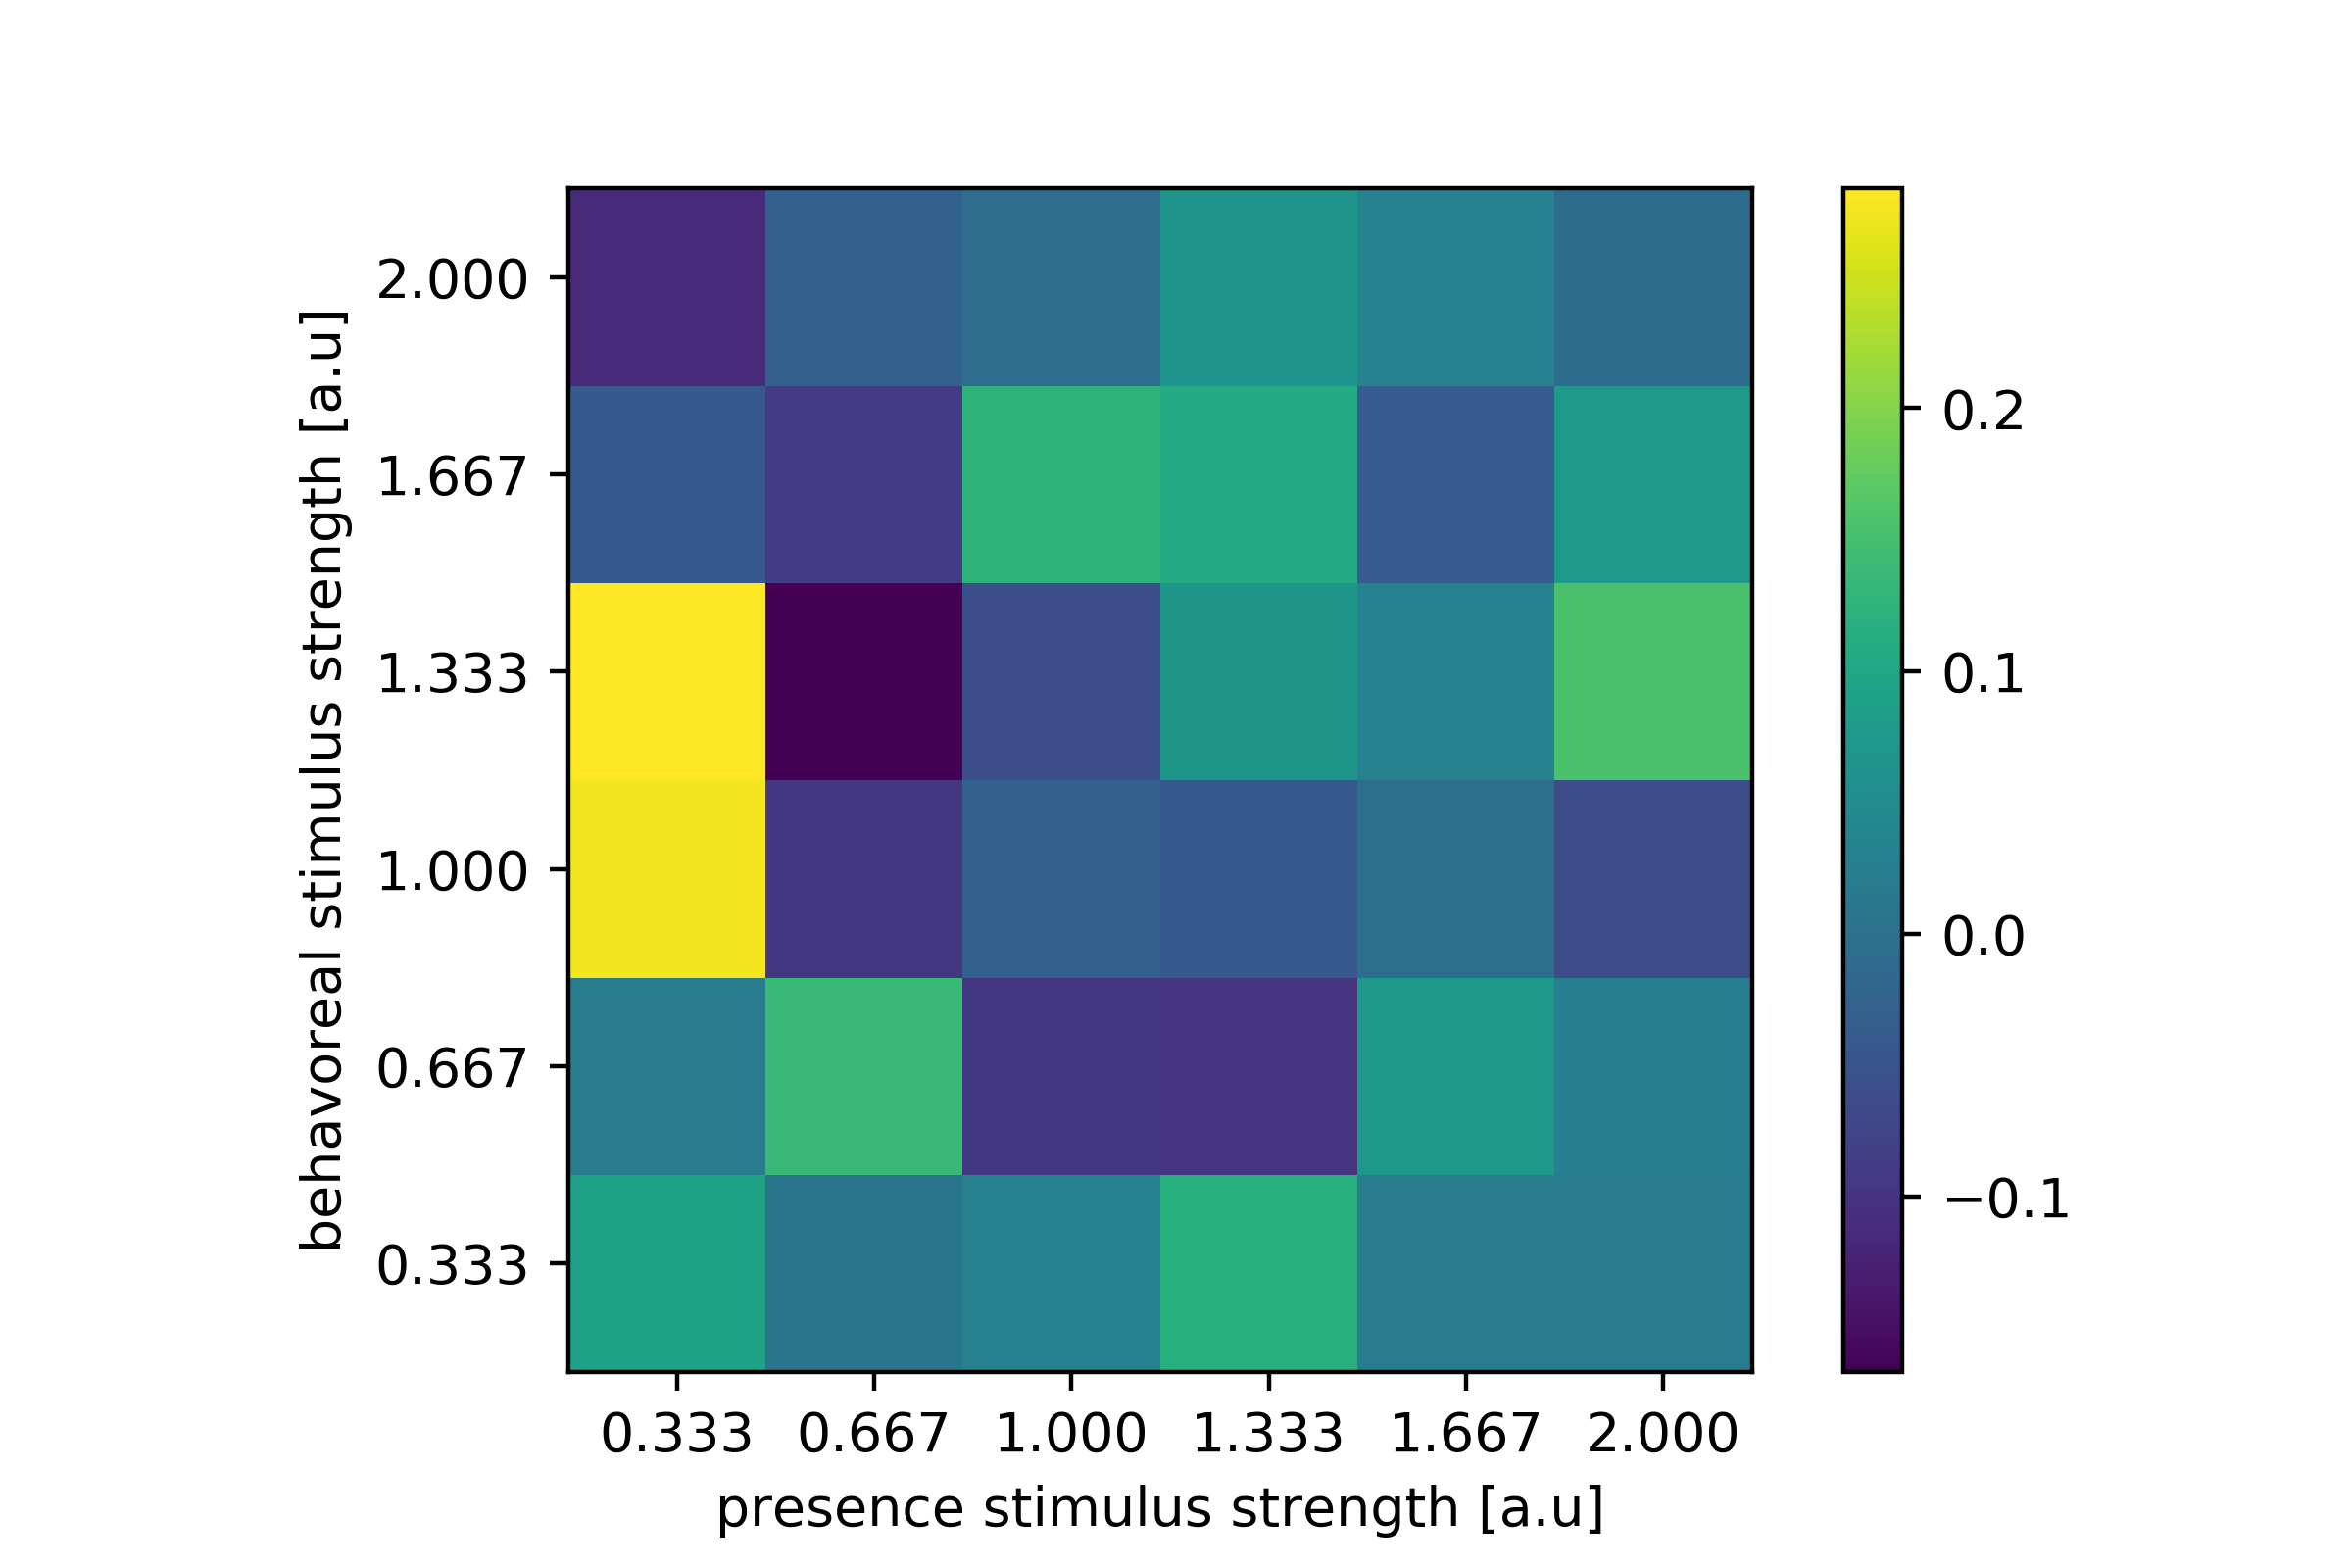
\includegraphics[width=1.0\textwidth]{transrank.png}
	\end{figure}
	\end{center}
\end{frame}

\begin{frame}[fragile]{Statistical Significance - Stimulus Presence}
\begin{center}
	\begin{figure}
      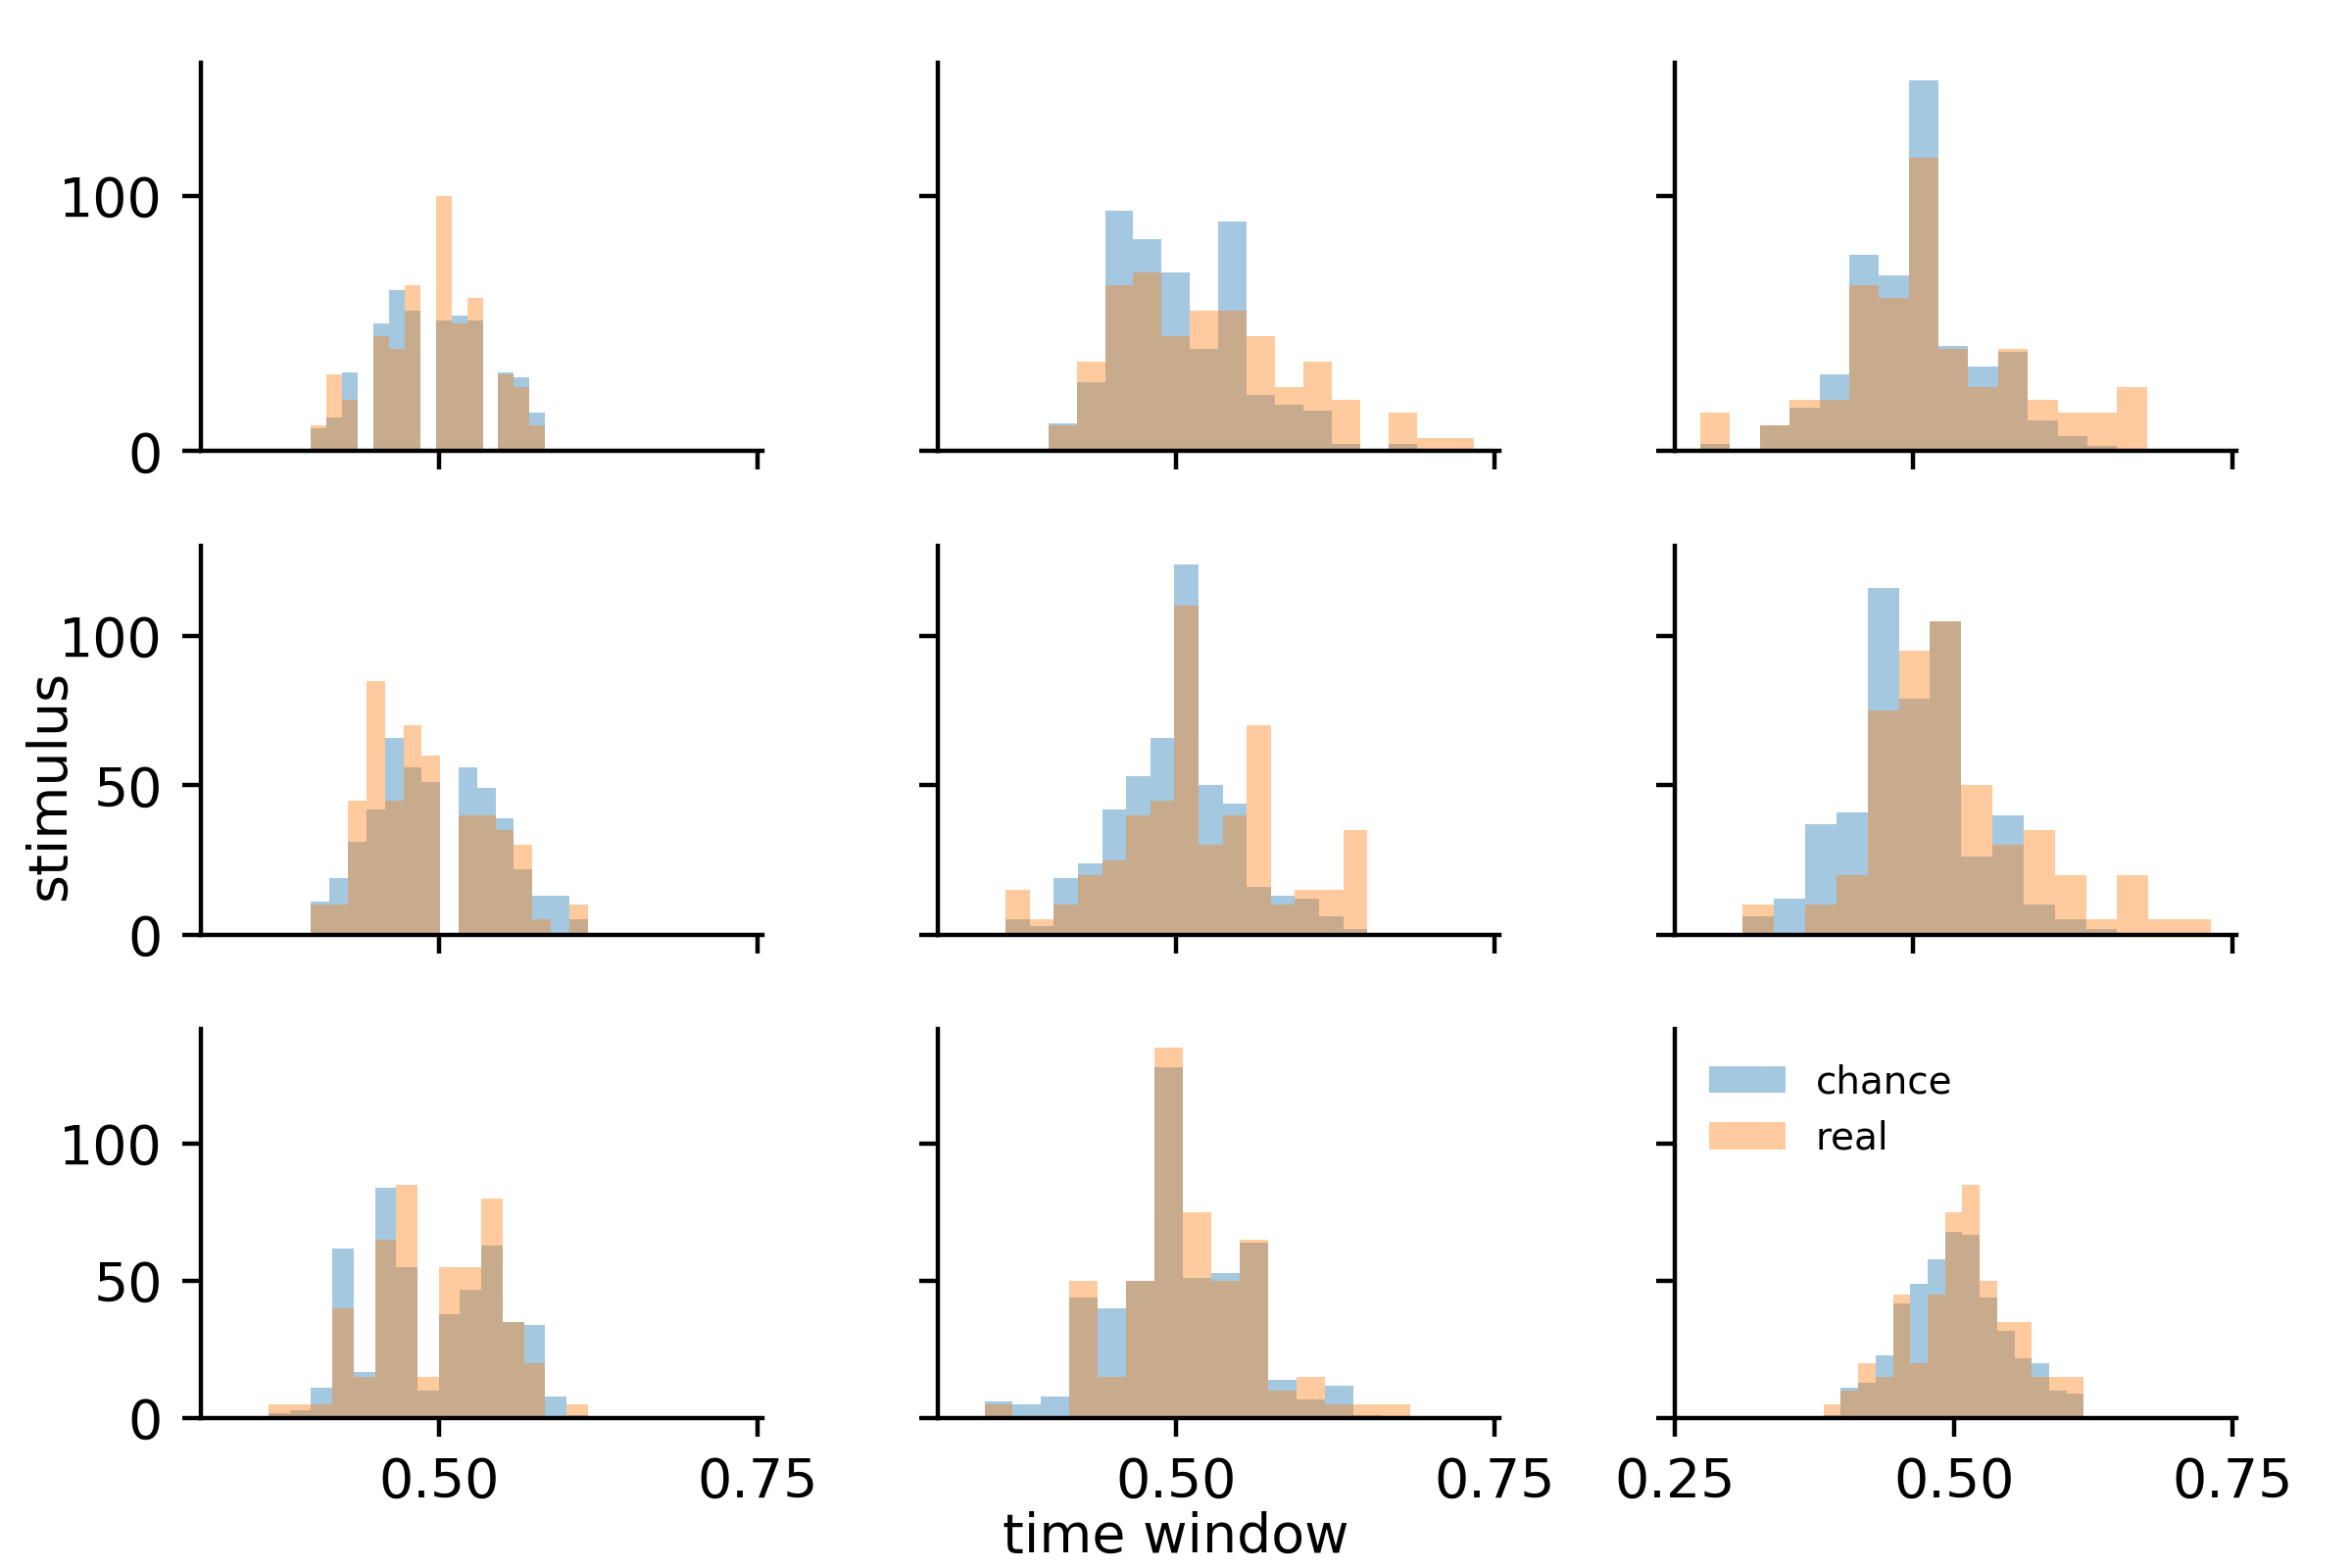
\includegraphics[width=1.0\textwidth]{statsig.png}
	\end{figure}
	\end{center}
\end{frame}

\begin{frame}[fragile]{Statistical Significance - Behavior}
At threshold stimulus $\approx$ 1
\begin{center}
	\begin{figure}
      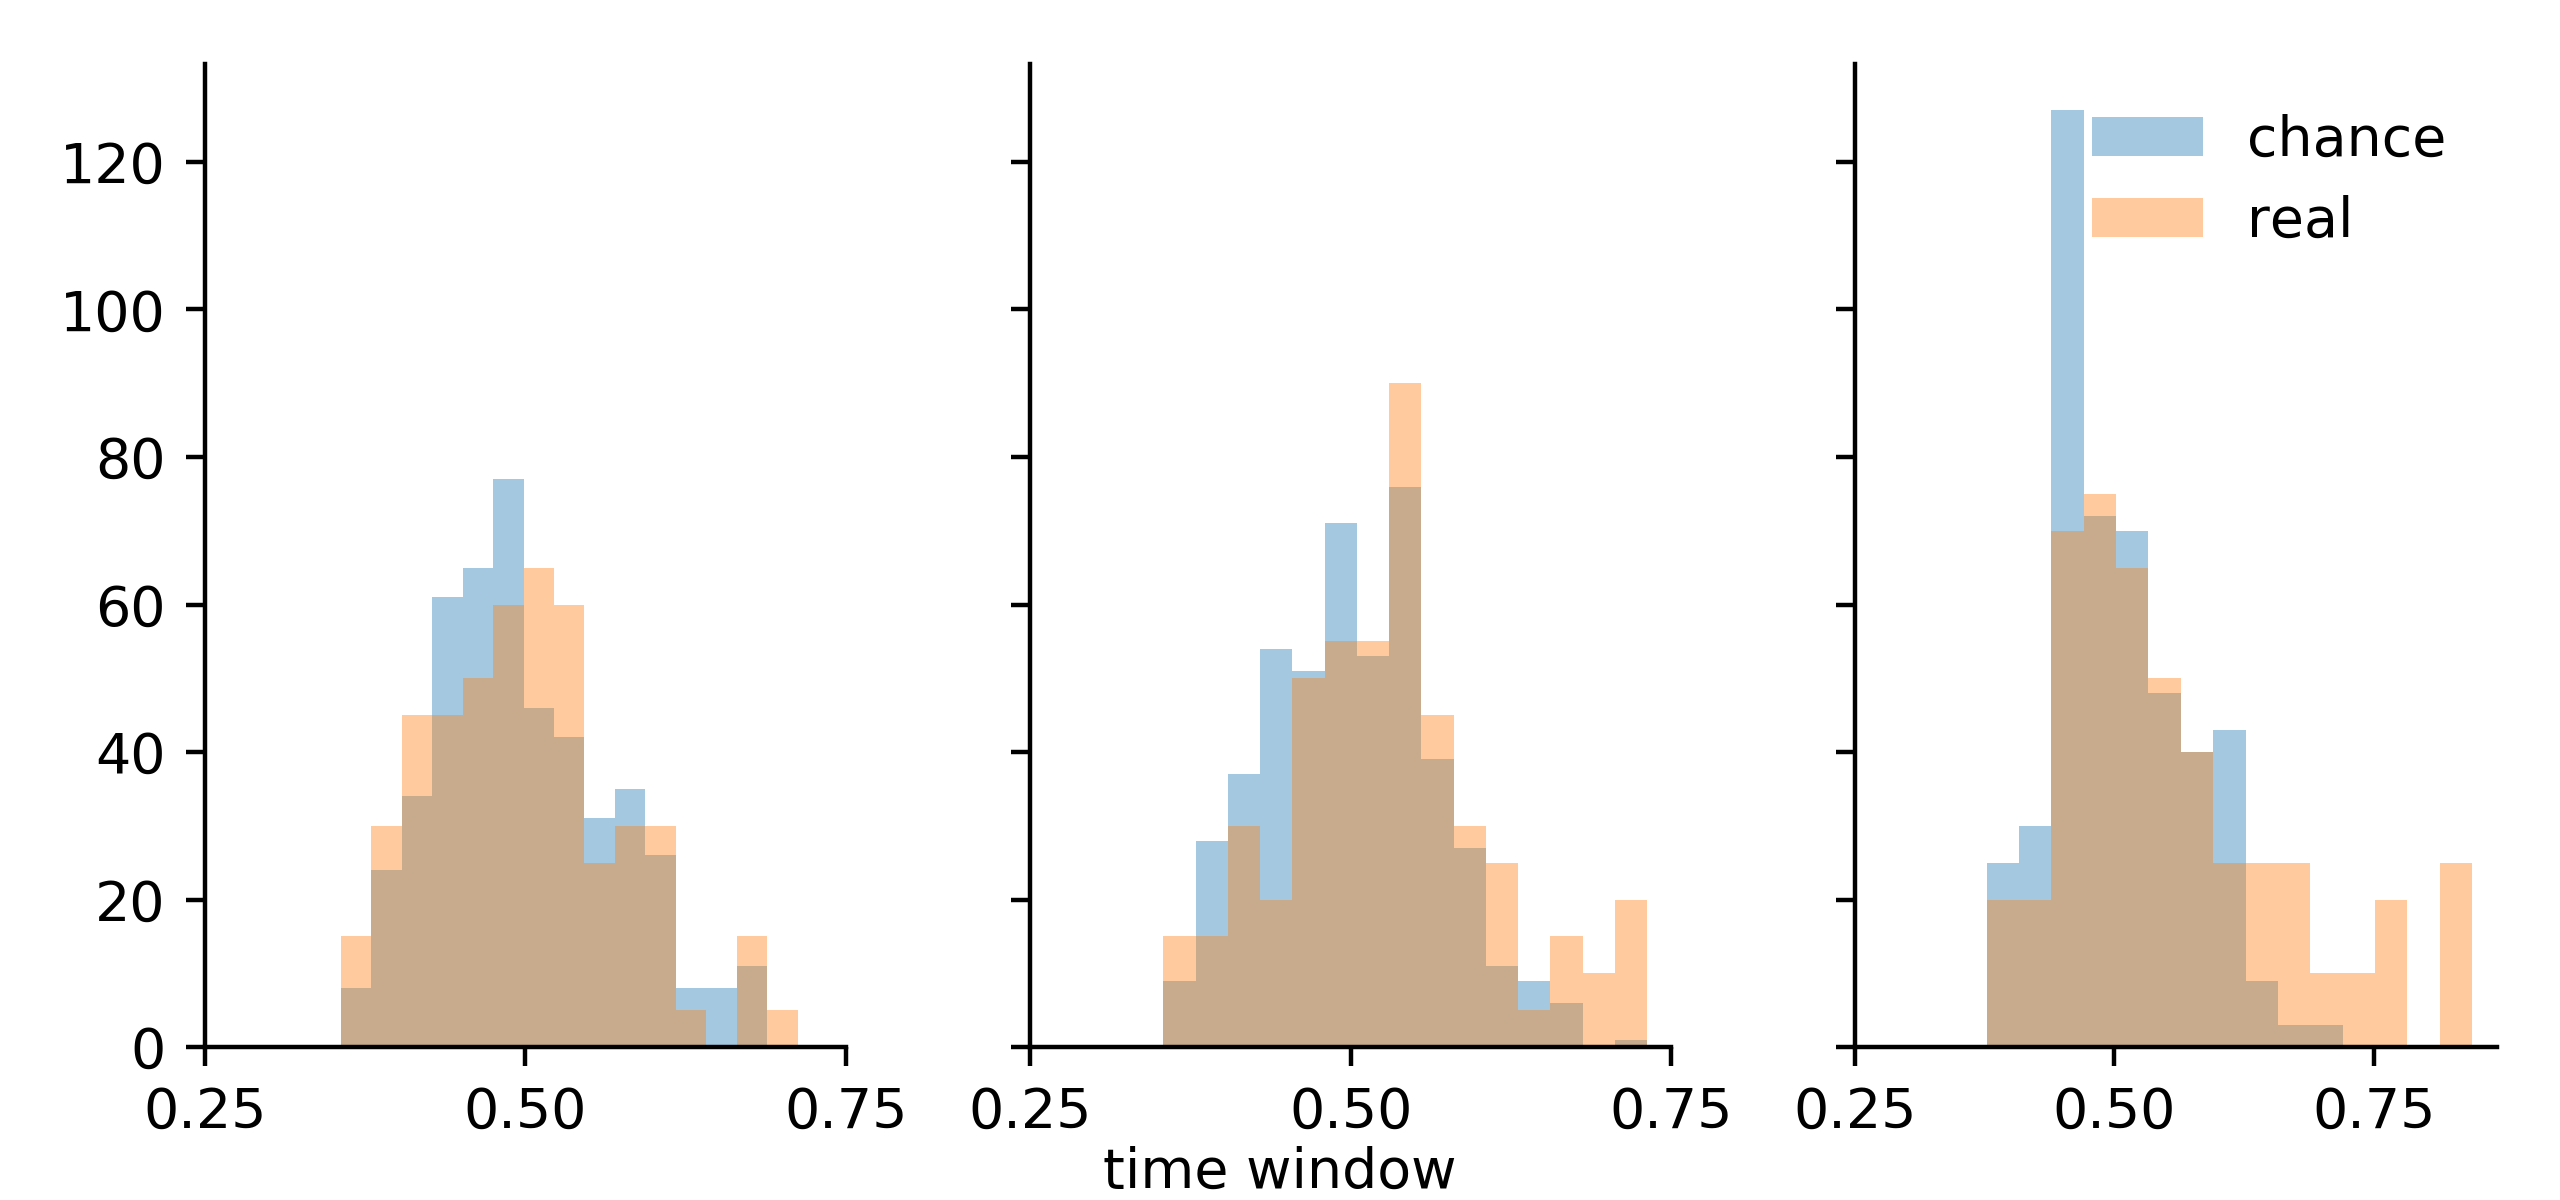
\includegraphics[width=1.0\textwidth]{statsig_b.png}
	\end{figure}
	\end{center}
\end{frame}

\section{Multivariate SMV Analysis}

\begin{frame}[fragile]{Presence Detection - Feature Selection}
\only<+->{
Since we have only few datapoints per condition (30-50 per class) in comparison to the number of features (100-150), we are prone to overfit to noise.}

\only<+->{
$\Rightarrow$ we have to do \textbf{feature selection}.}

\only<+->{
We can use the previously best discriminating dendrites (SVM/DI).}
\end{frame}

\begin{frame}[fragile]{DI and SVM Dendrite Rank Order Correlation}
\begin{center}
	\begin{figure}
	%\caption*{todo: tens, improve weights}
      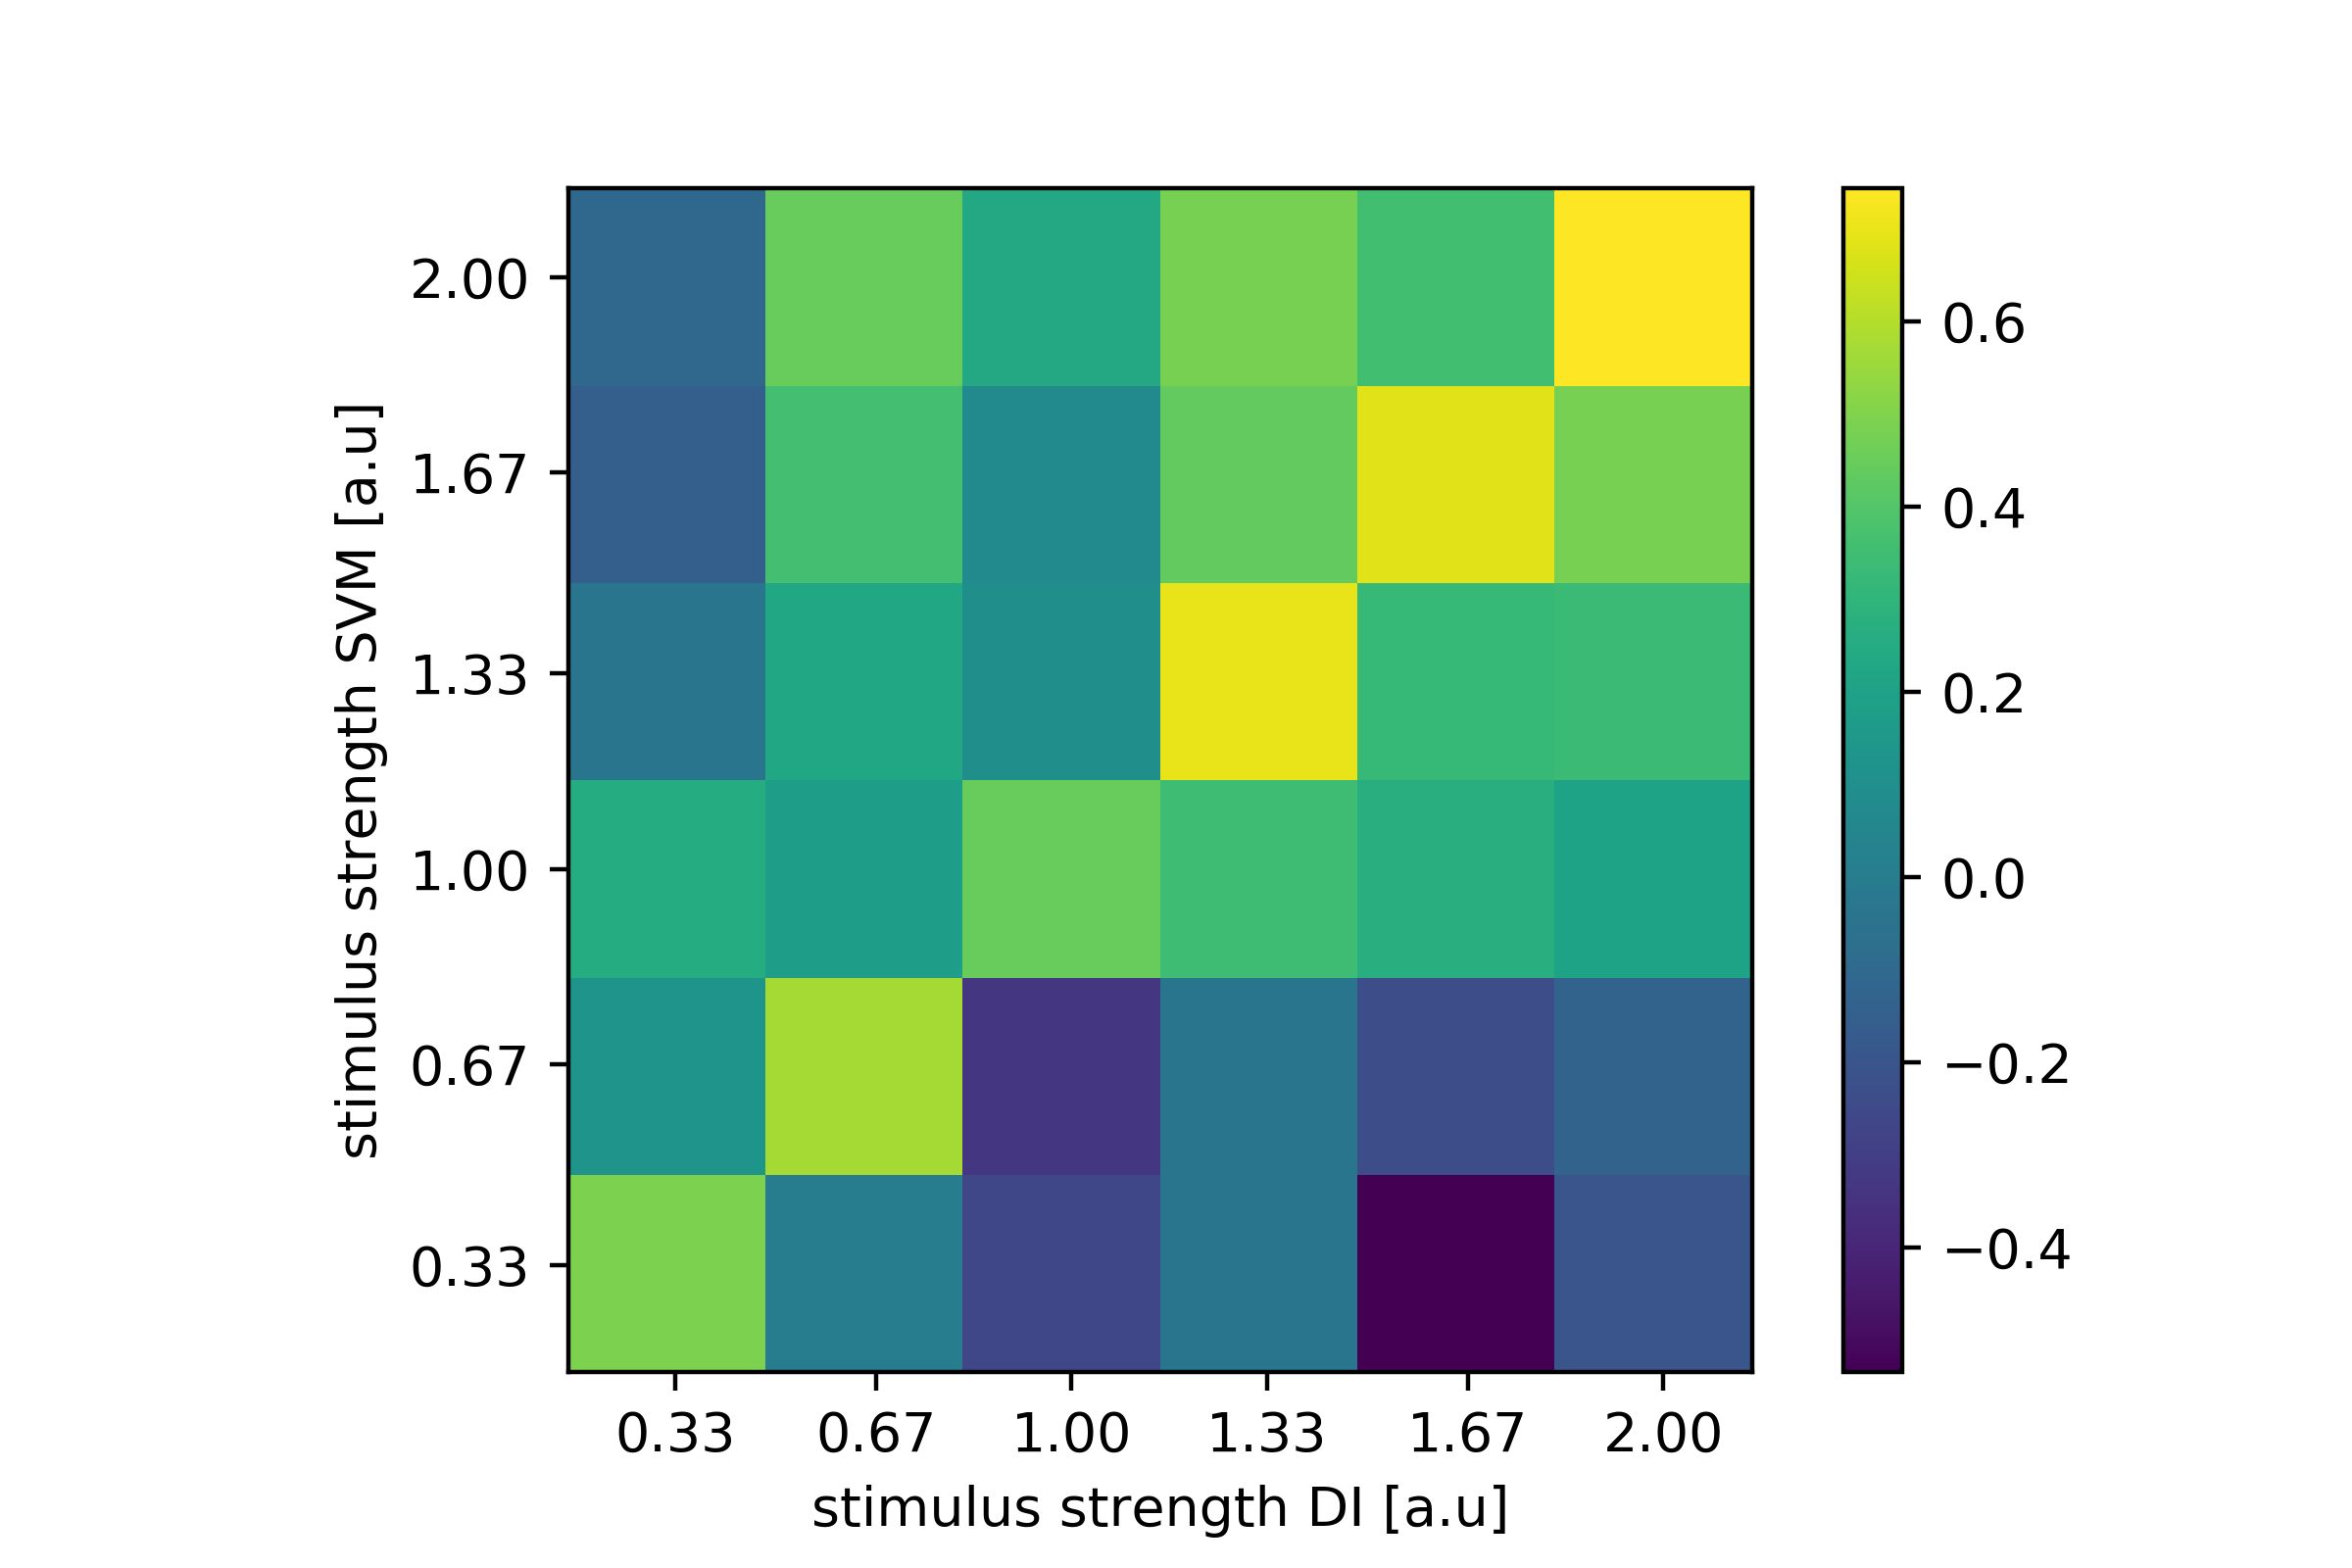
\includegraphics[width=1.0\textwidth]{rank_DI_SVM.png}
	\end{figure}
	\end{center}
\end{frame}

\begin{frame}[fragile]{SVM Performance on Combined Dendrites - Presence Detection}
\begin{center}
	\begin{figure}
	%\caption*{todo: tens, improve weights}
      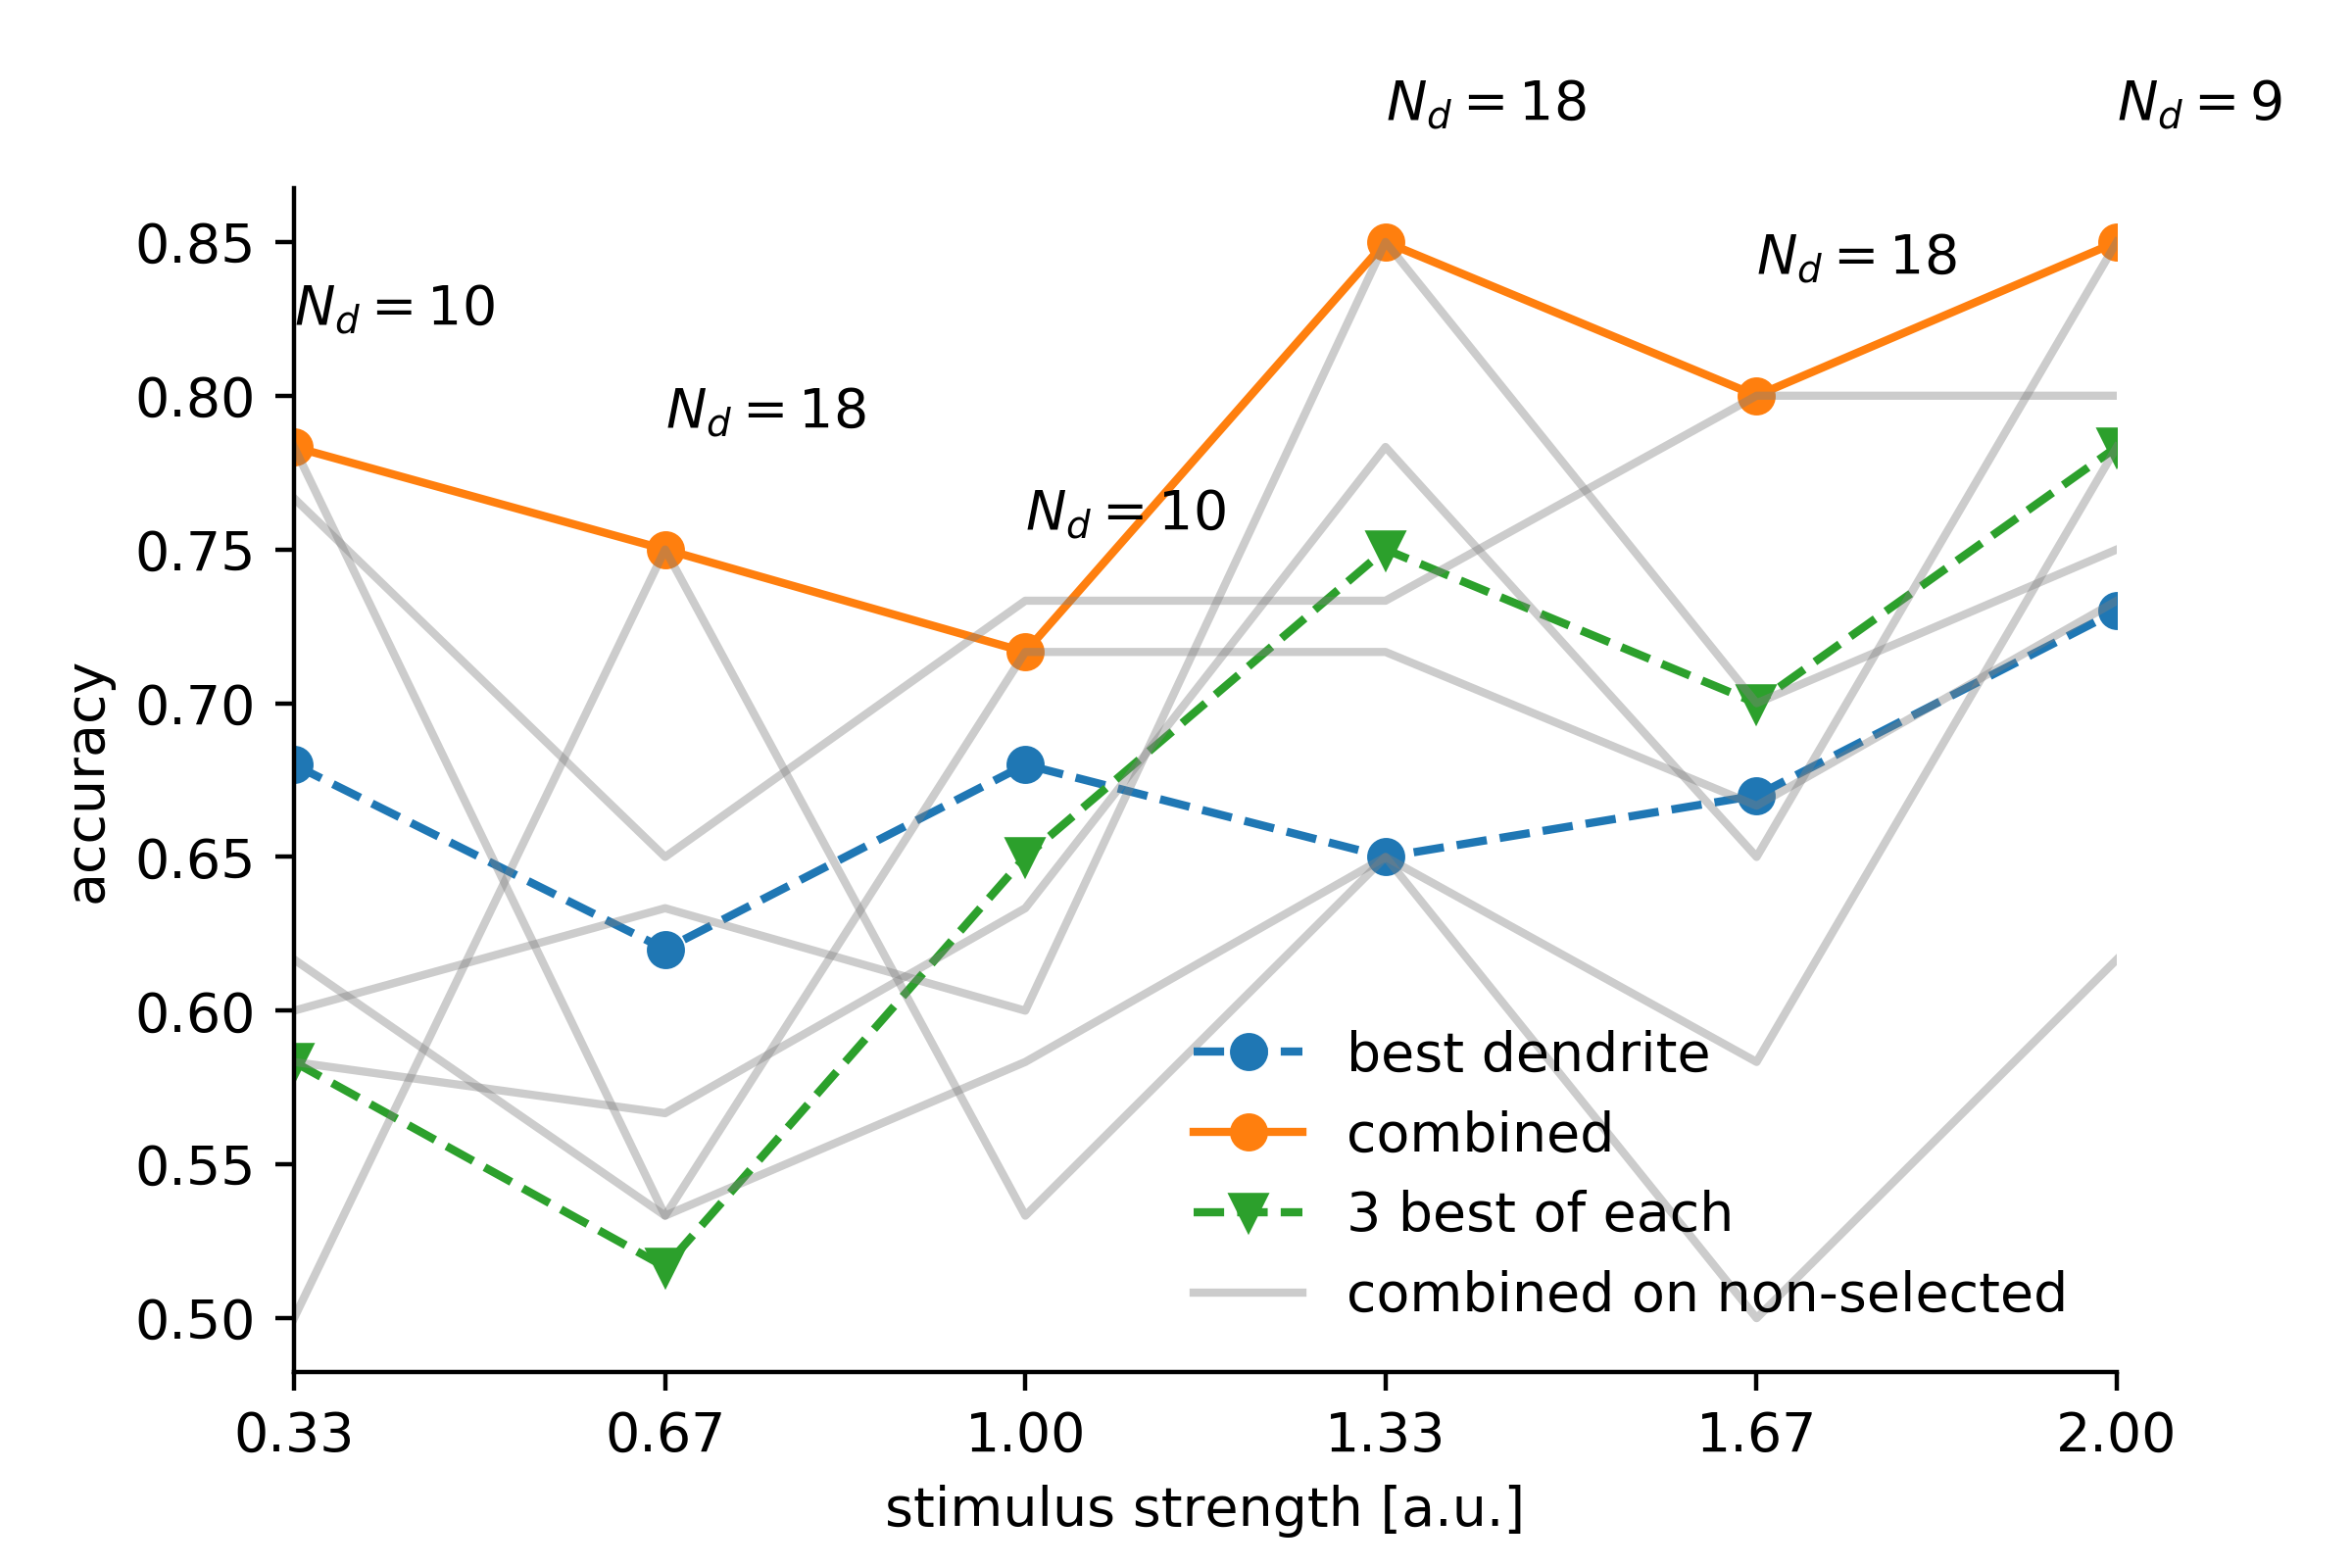
\includegraphics[width=1.0\textwidth]{combined_presence.png}
	\end{figure}
	\end{center}
\end{frame}

\begin{frame}[fragile]{SVM Performance on Combined Dendrites - Global Presence}
\begin{center}
	\begin{figure}
	%\caption*{todo: tens, improve weights}
      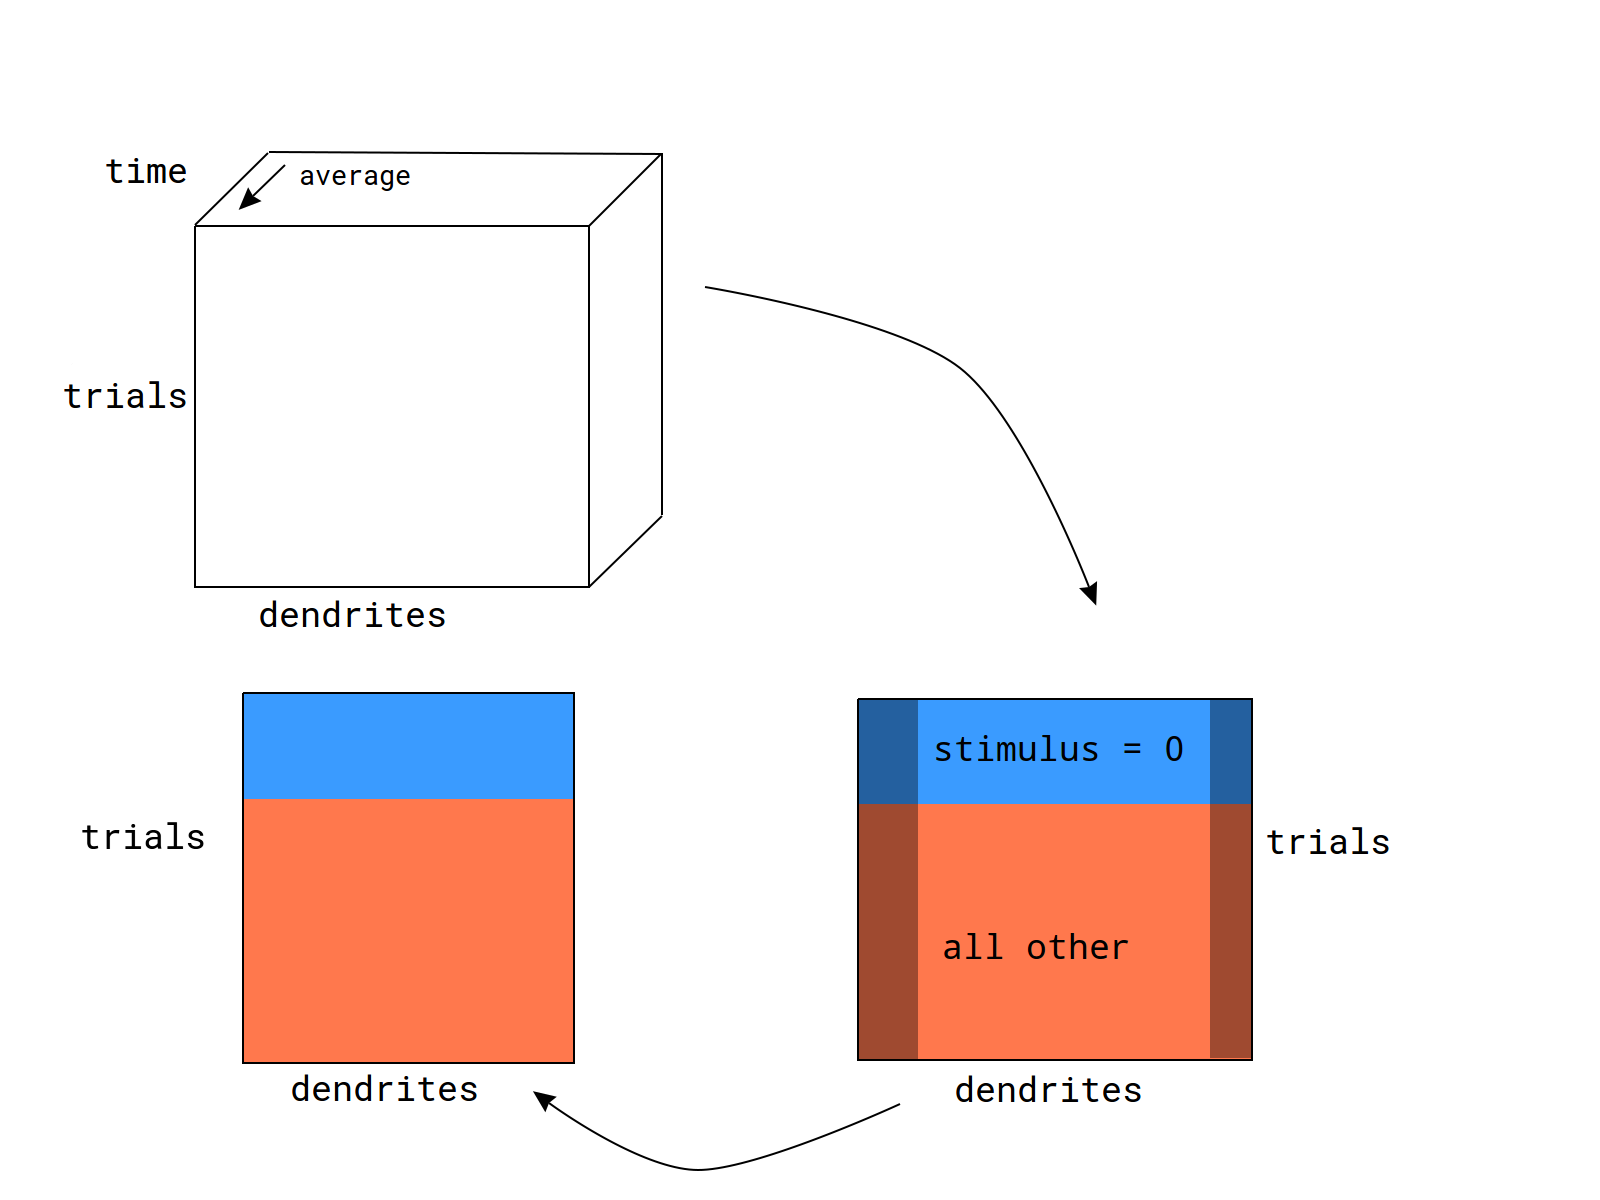
\includegraphics[width=1.0\textwidth]{data_p_tot.png}
	\end{figure}
	\end{center}
\end{frame}

\begin{frame}[fragile]{SVM Performance on Combined Dendrites - Global Presence}
Performance on global presence detection: \newline
Mean: 0.68 \newline
Standard deviation: 0.08
\end{frame}

\begin{frame}[fragile]{SVM Performance on Combined Dendrites - Presence Detection}
\begin{center}
	\begin{figure}
	%\caption*{todo: tens, improve weights}
      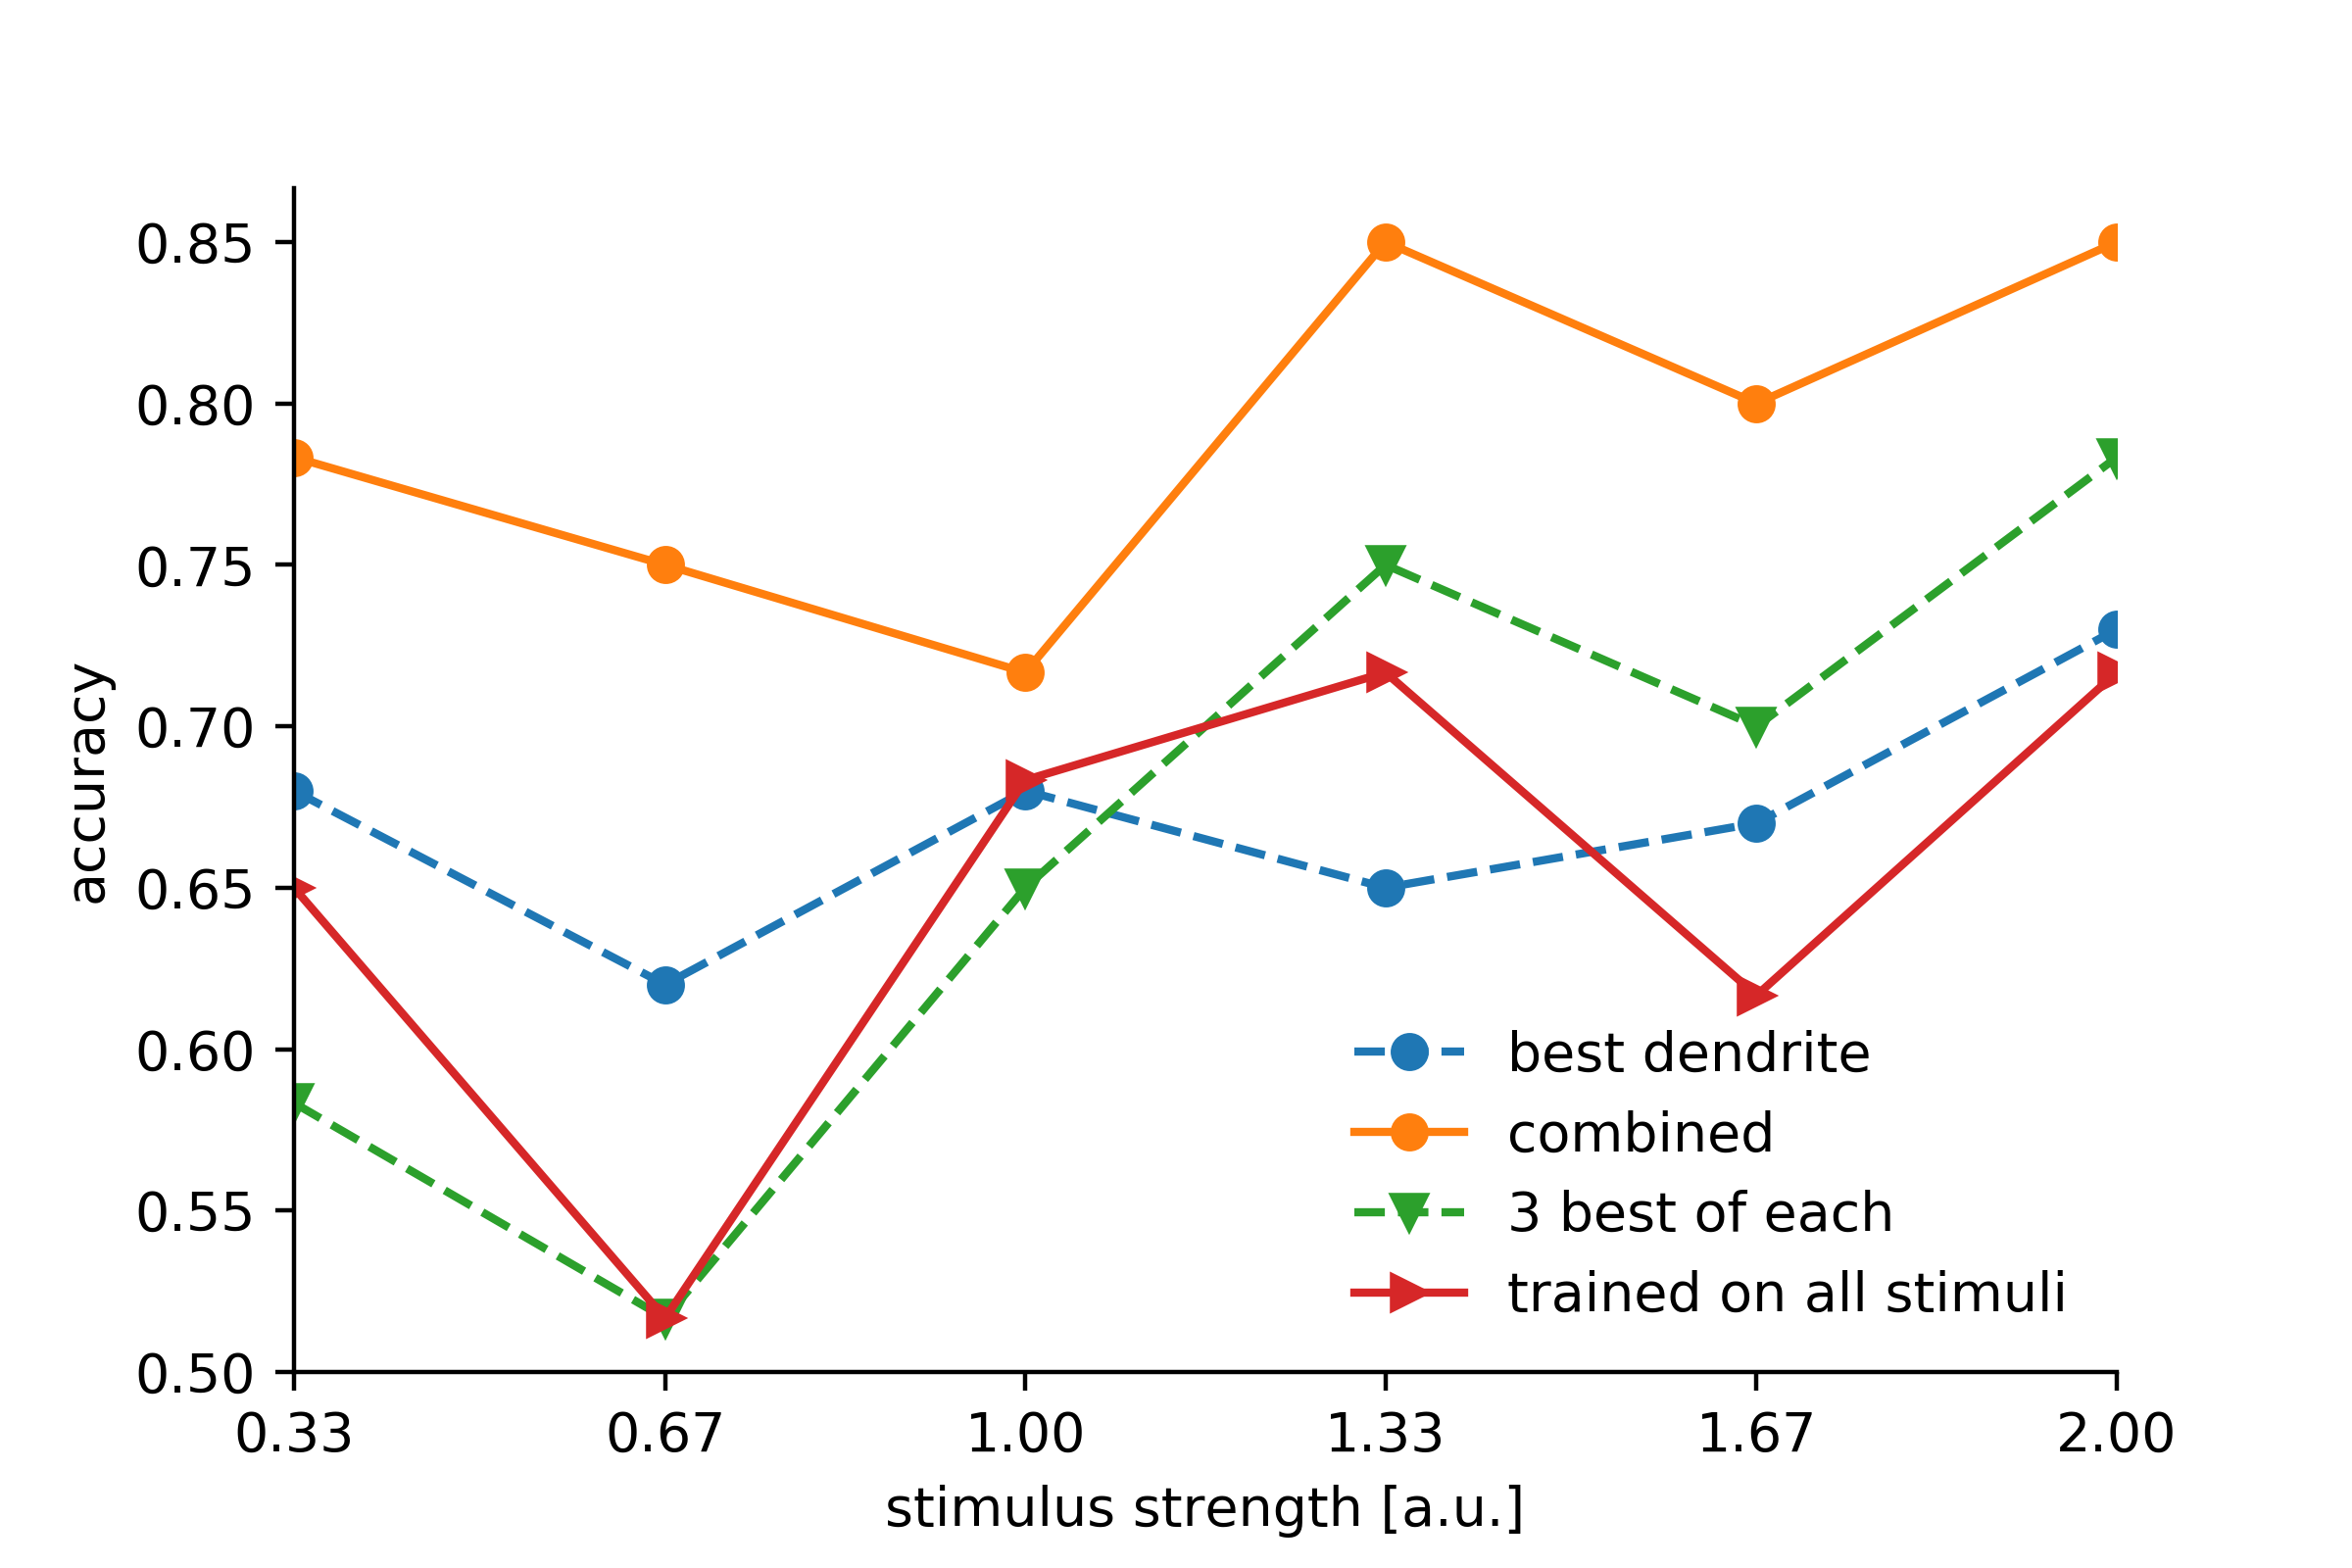
\includegraphics[width=1.0\textwidth]{combined_presence_alt.png}
	\end{figure}
	\end{center}
\end{frame}

\begin{frame}[fragile]{SVM Performance on Combined Dendrites - Global Behavior}
\begin{center}
	\begin{figure}
	%\caption*{todo: tens, improve weights}
      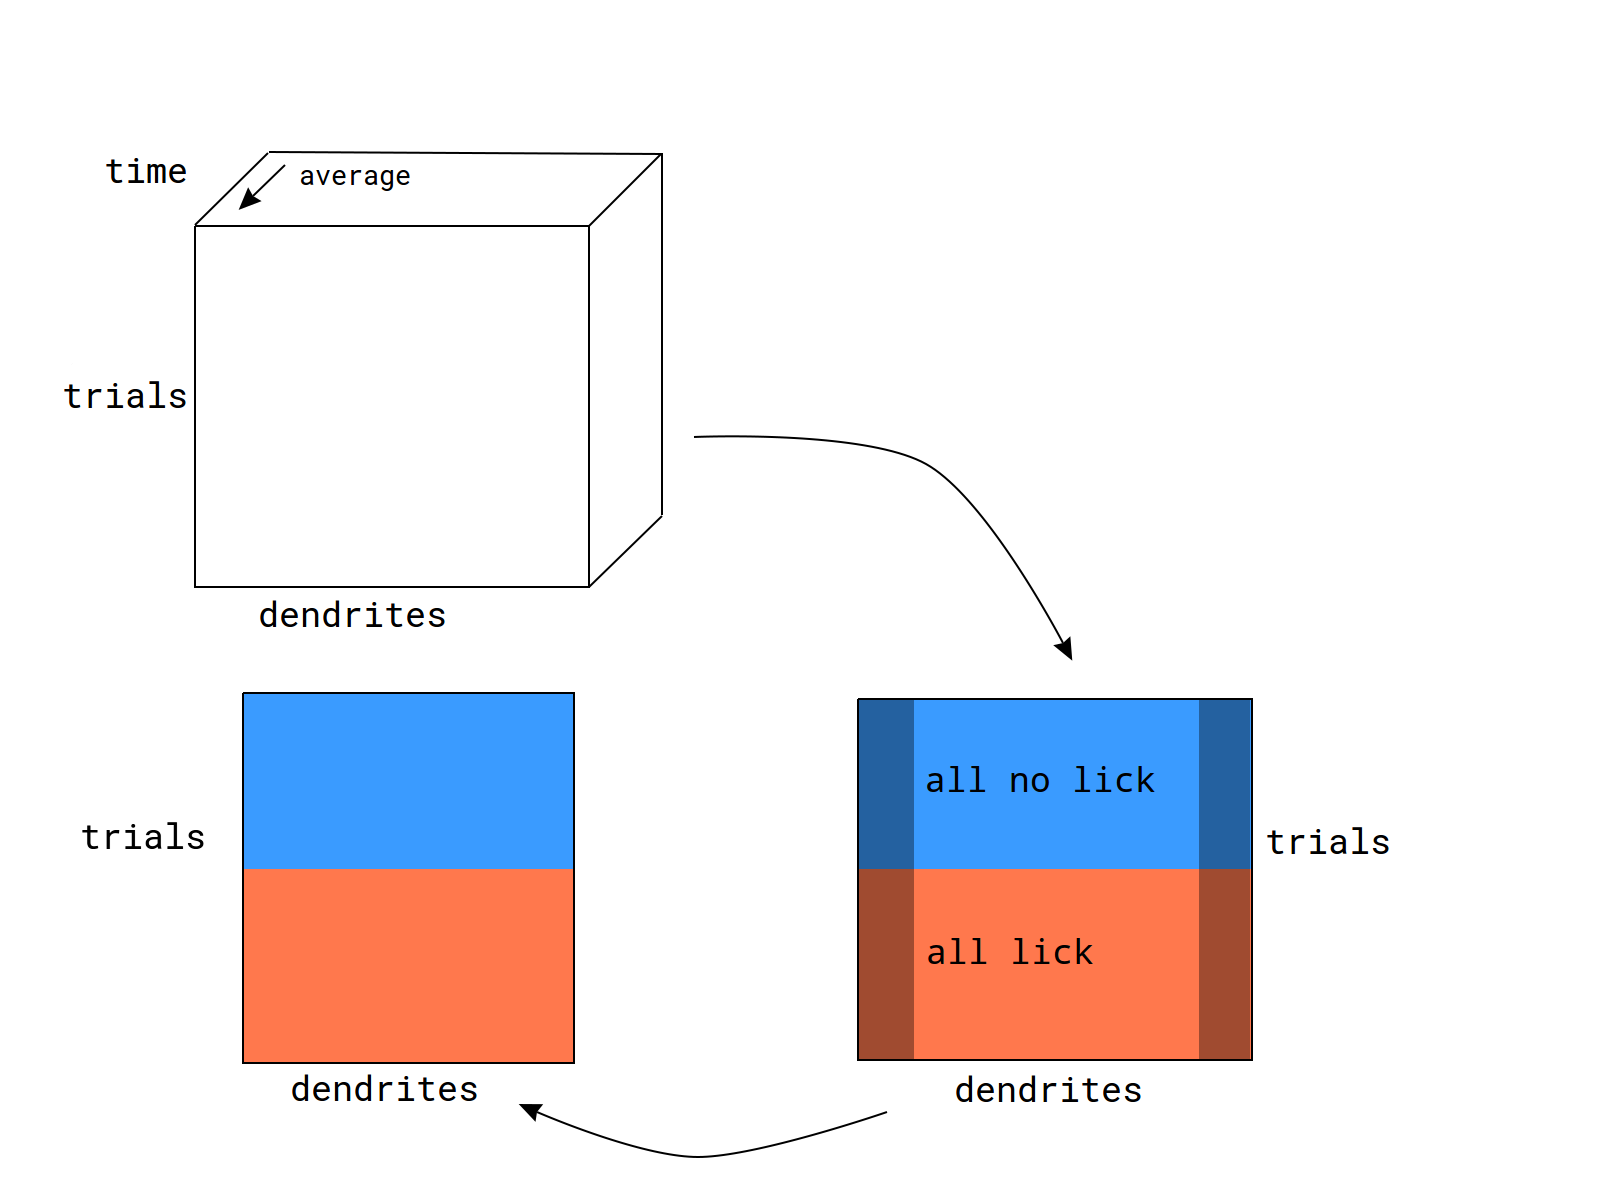
\includegraphics[width=1.0\textwidth]{data_hm_tot.png}
	\end{figure}
	\end{center}
\end{frame}

\begin{frame}[fragile]{SVM Performance on Combined Dendrites - Global Behavior}
Performance on global presence detection: \newline
Mean: 0.71 \newline
Standard deviation: 0.1
\end{frame}

\begin{frame}[fragile]{SVM Performance on Combined Dendrites - Behavioral}
\begin{center}
	\begin{figure}
	%\caption*{todo: tens, improve weights}
      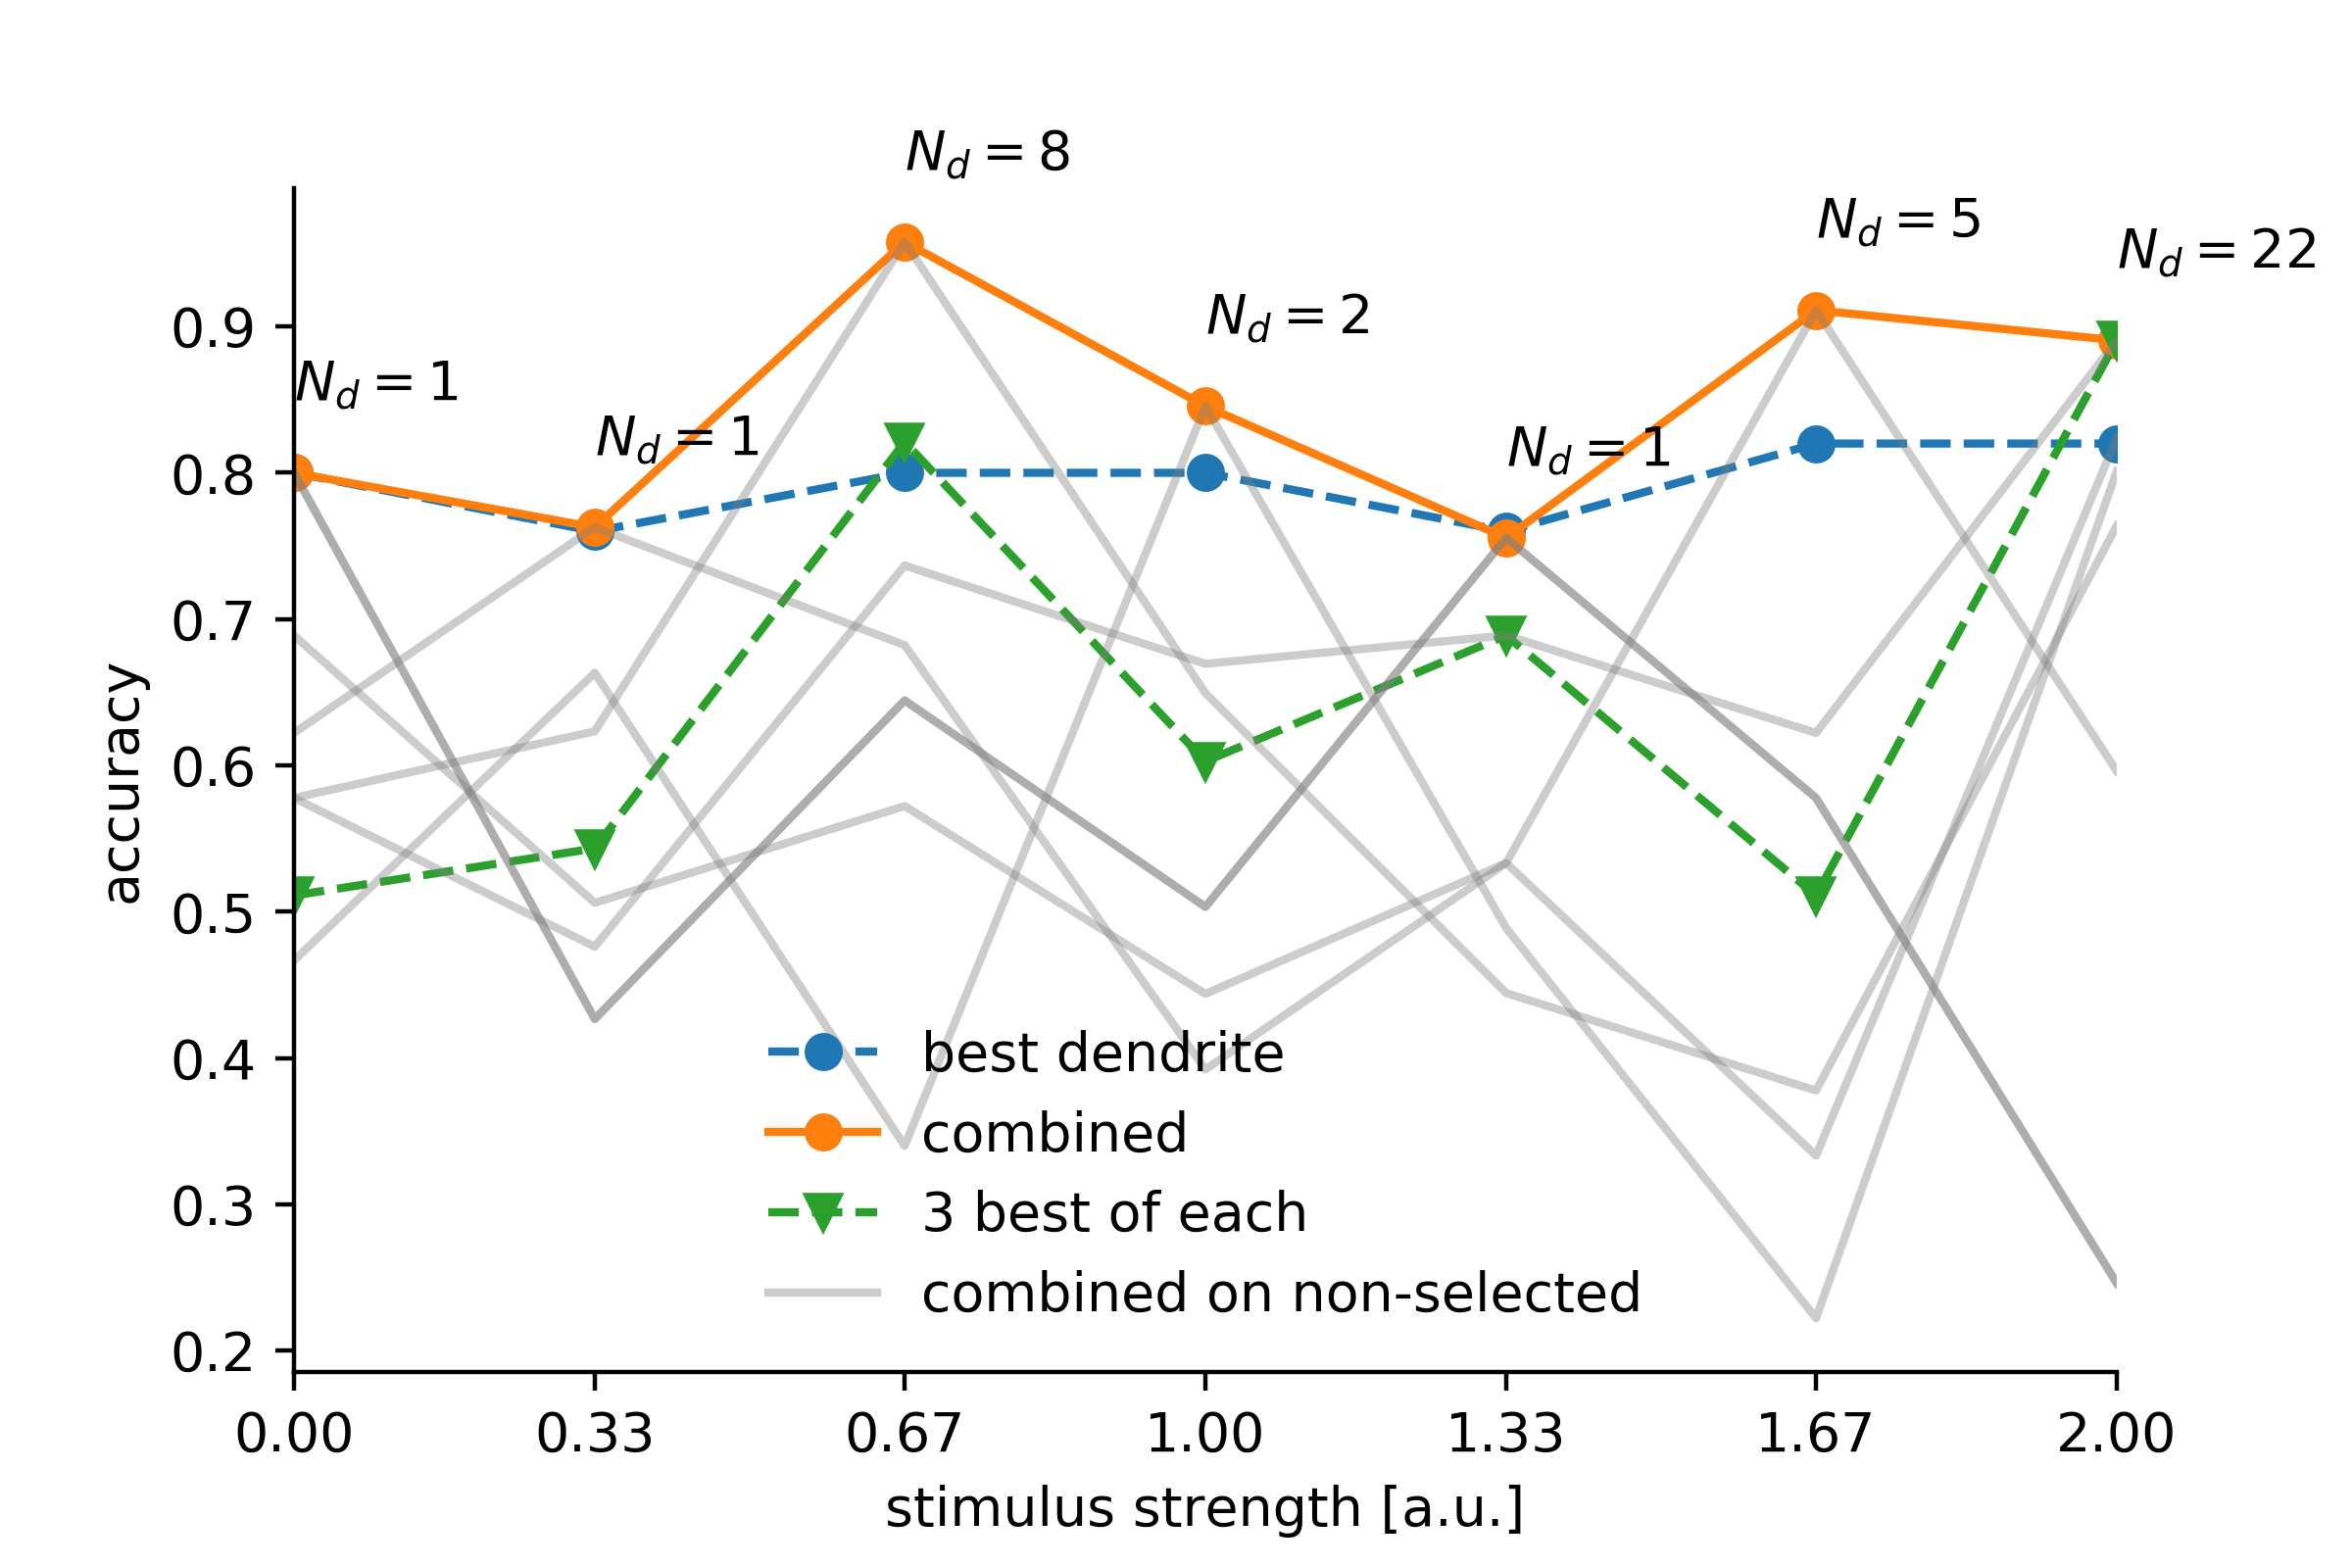
\includegraphics[width=1.0\textwidth]{combined_hitmiss.png}
	\end{figure}
	\end{center}
\end{frame}

\begin{frame}[fragile]{SVM Performance on Combined Dendrites - Behavioral}
\begin{center}
	\begin{figure}
	%\caption*{todo: tens, improve weights}
      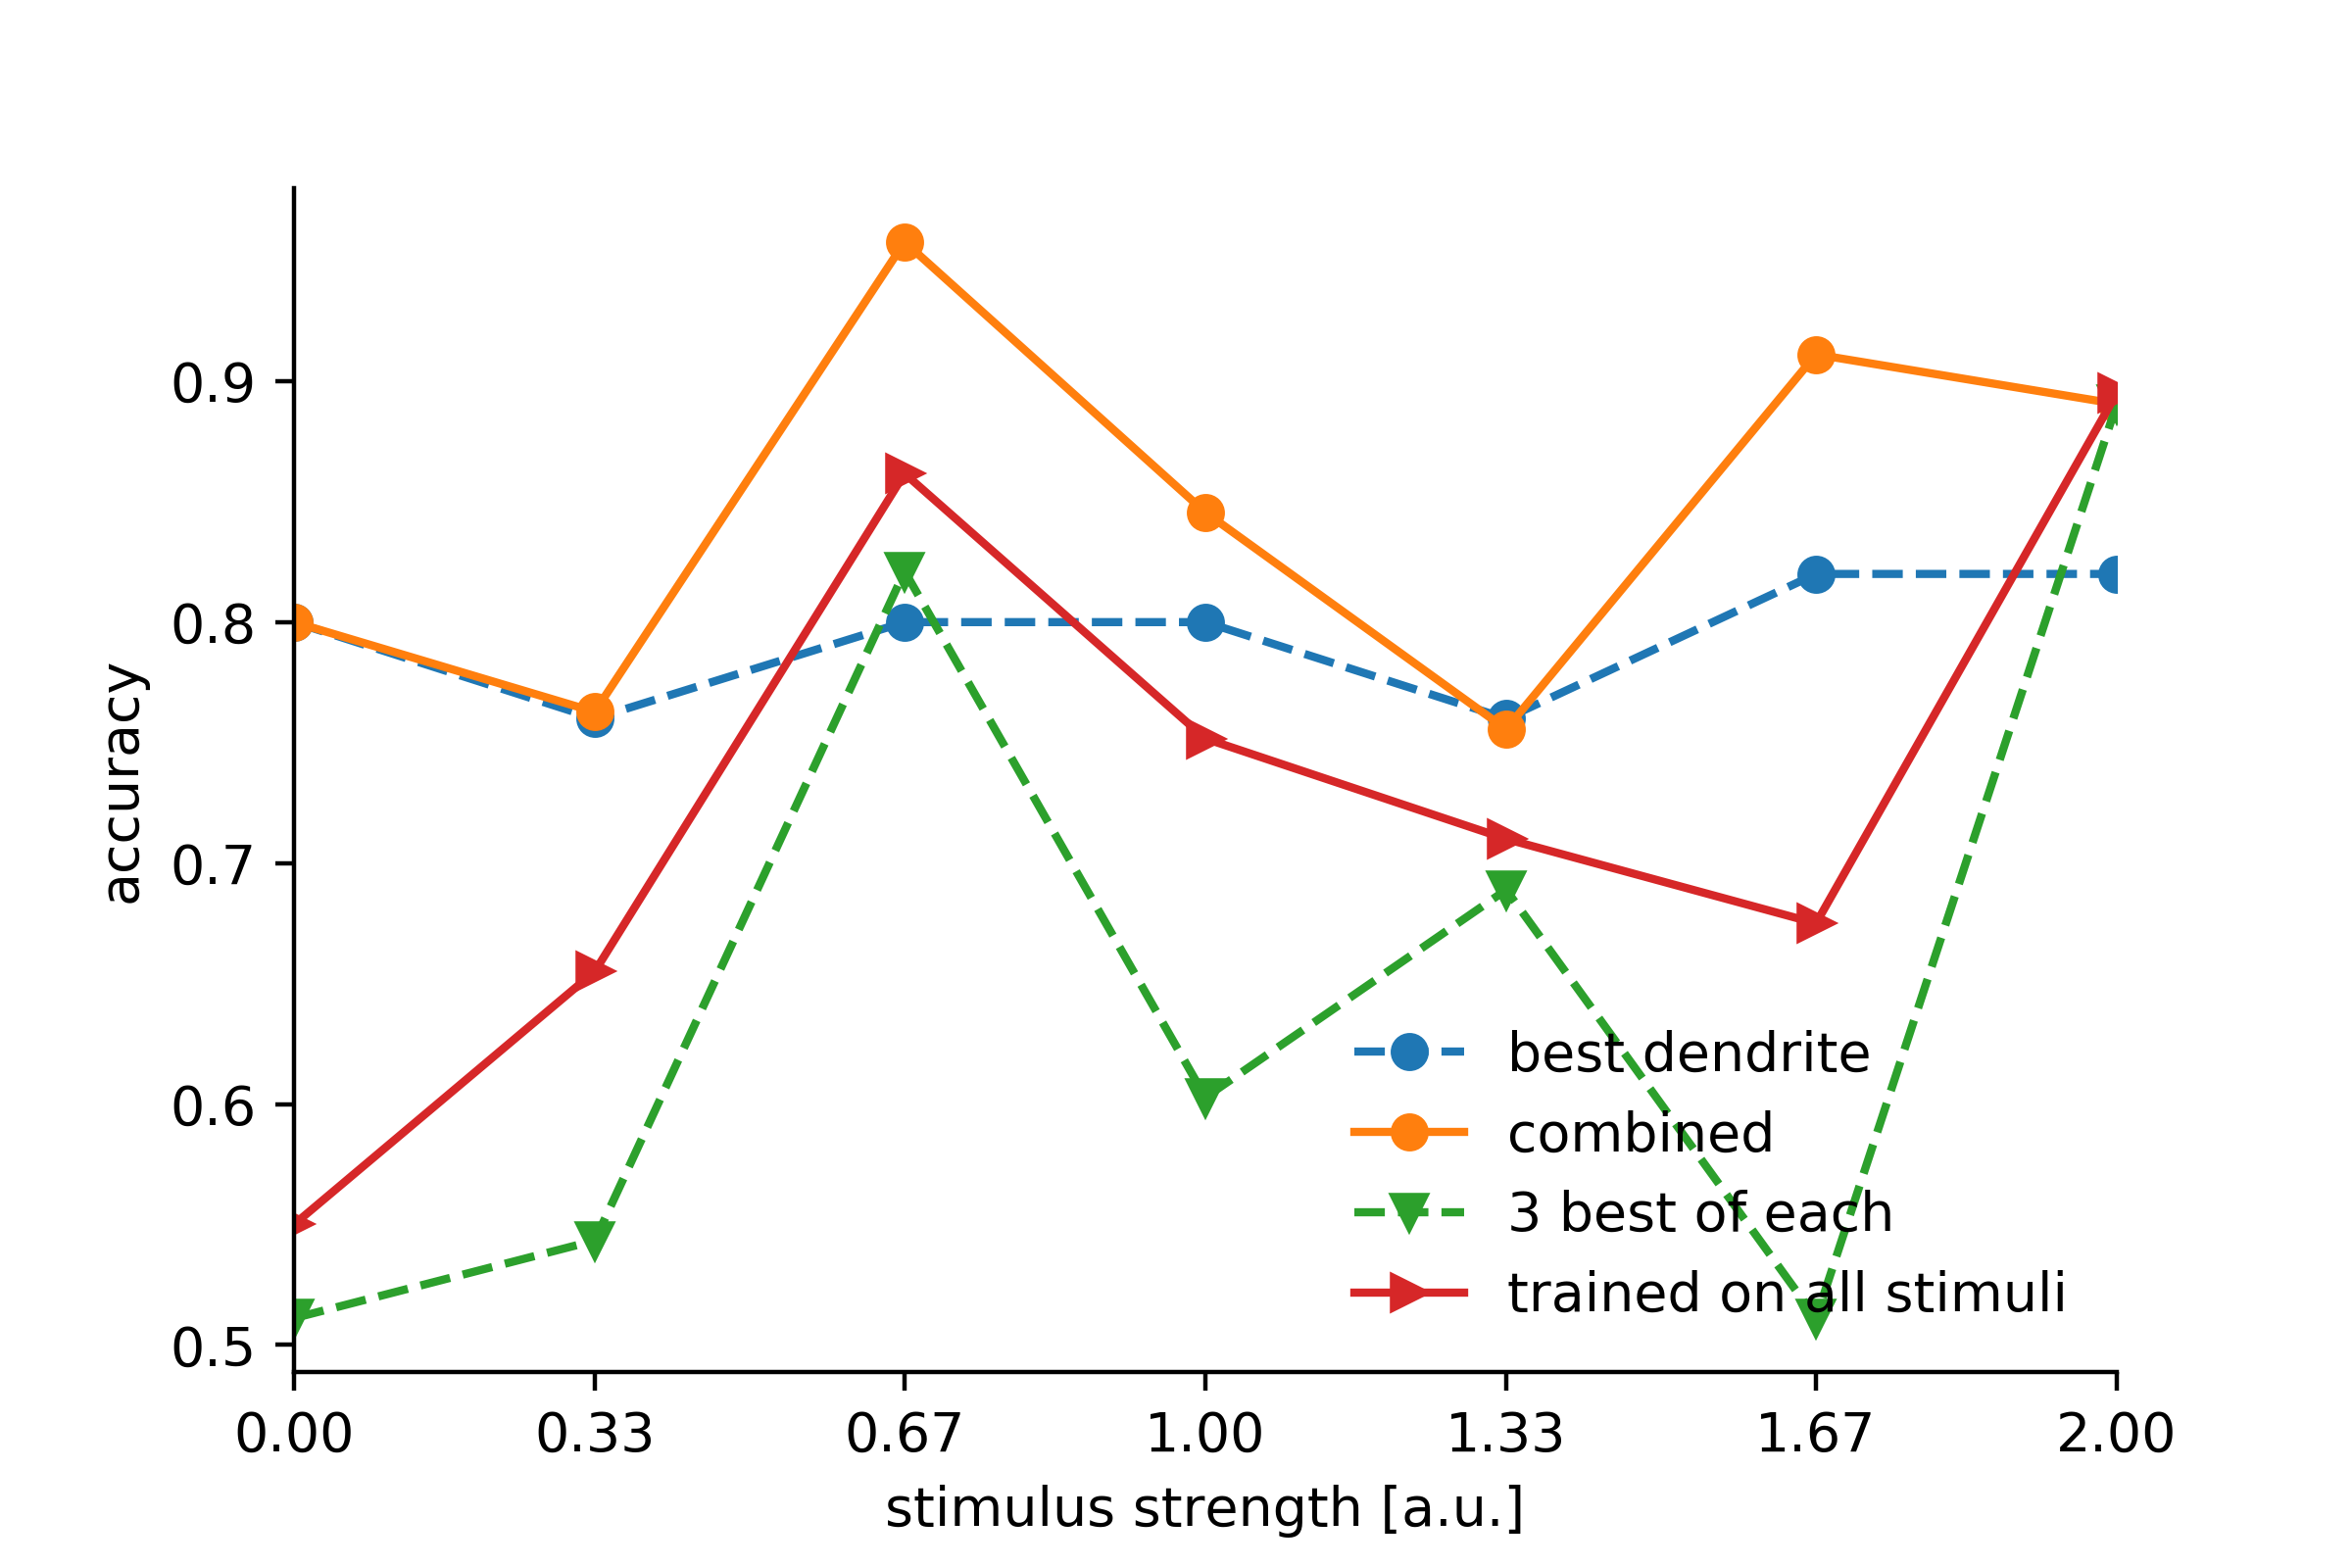
\includegraphics[width=1.0\textwidth]{combined_hitmiss_alt.png}
	\end{figure}
	\end{center}
\end{frame}

\begin{frame}[fragile]{Optimal Averaging Times}
\begin{center}
	\begin{figure}
	\caption*{Dummy}
      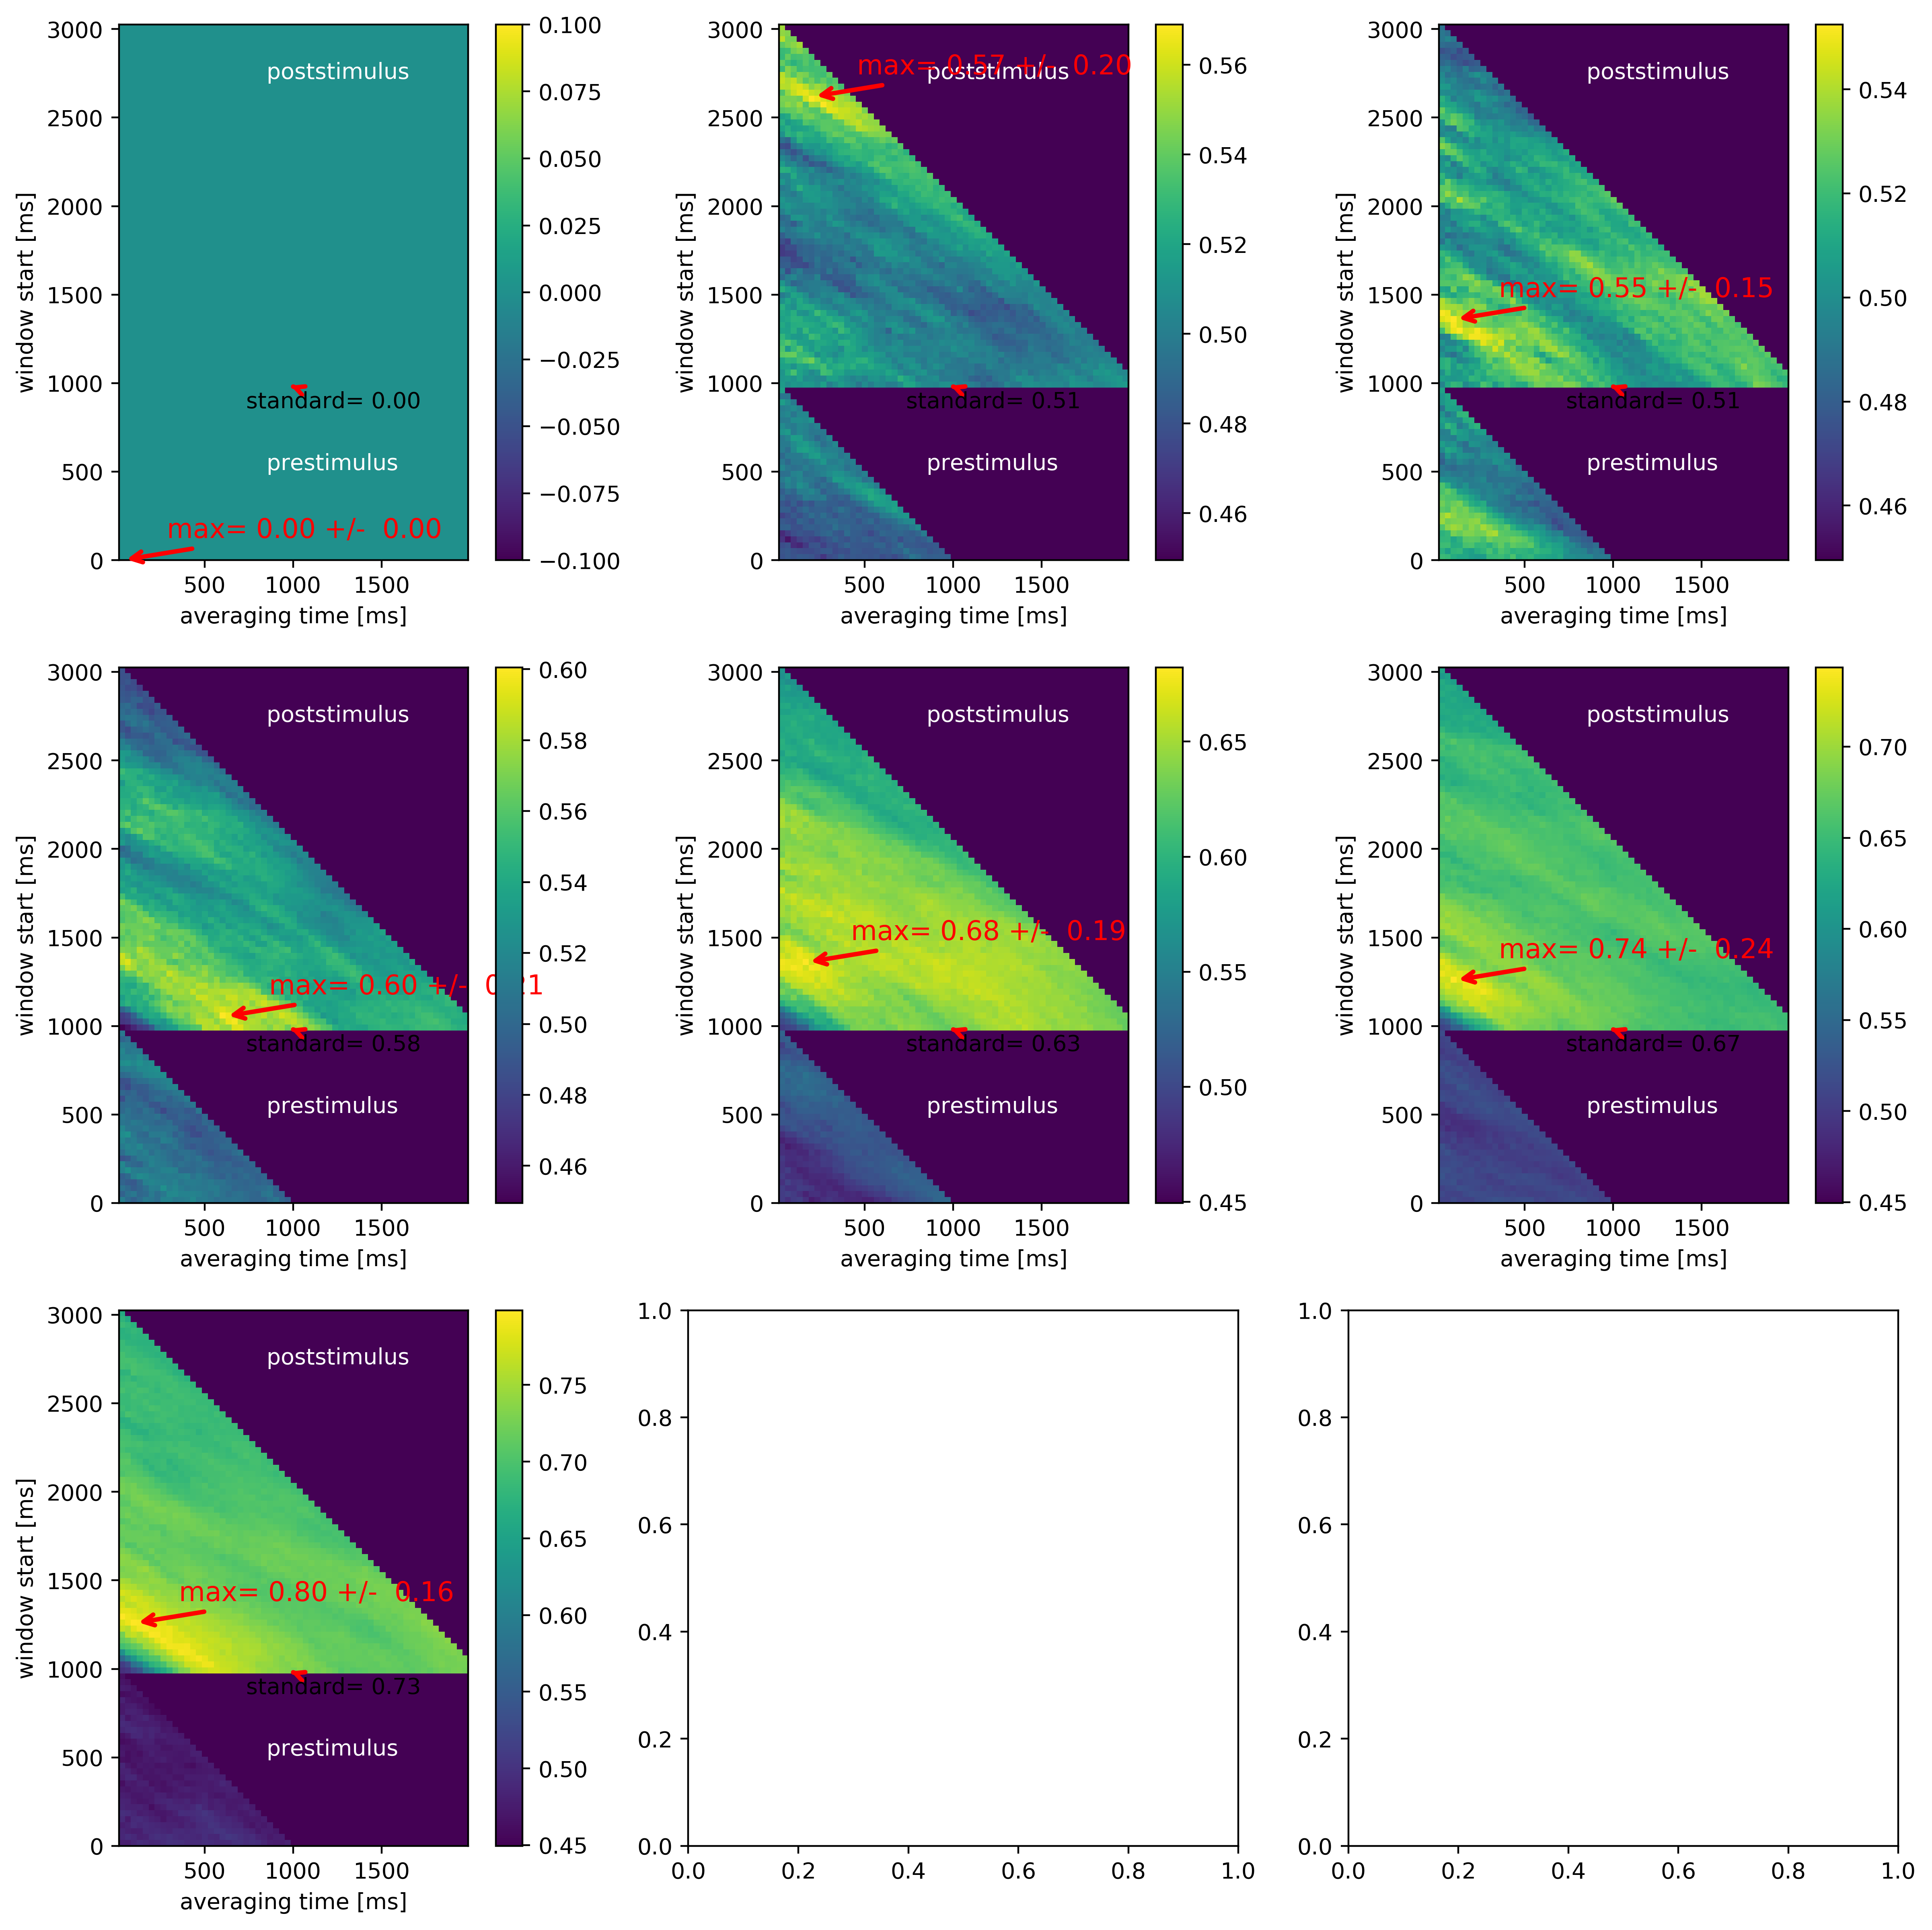
\includegraphics[width=0.6\textwidth]{placeholder_wind_pres.png}
	\end{figure}
	\end{center}
\end{frame}

\begin{frame}[fragile]{Optimal Averaging Times - Behavior}
\begin{center}
	\begin{figure}
	\caption*{Dummy}
      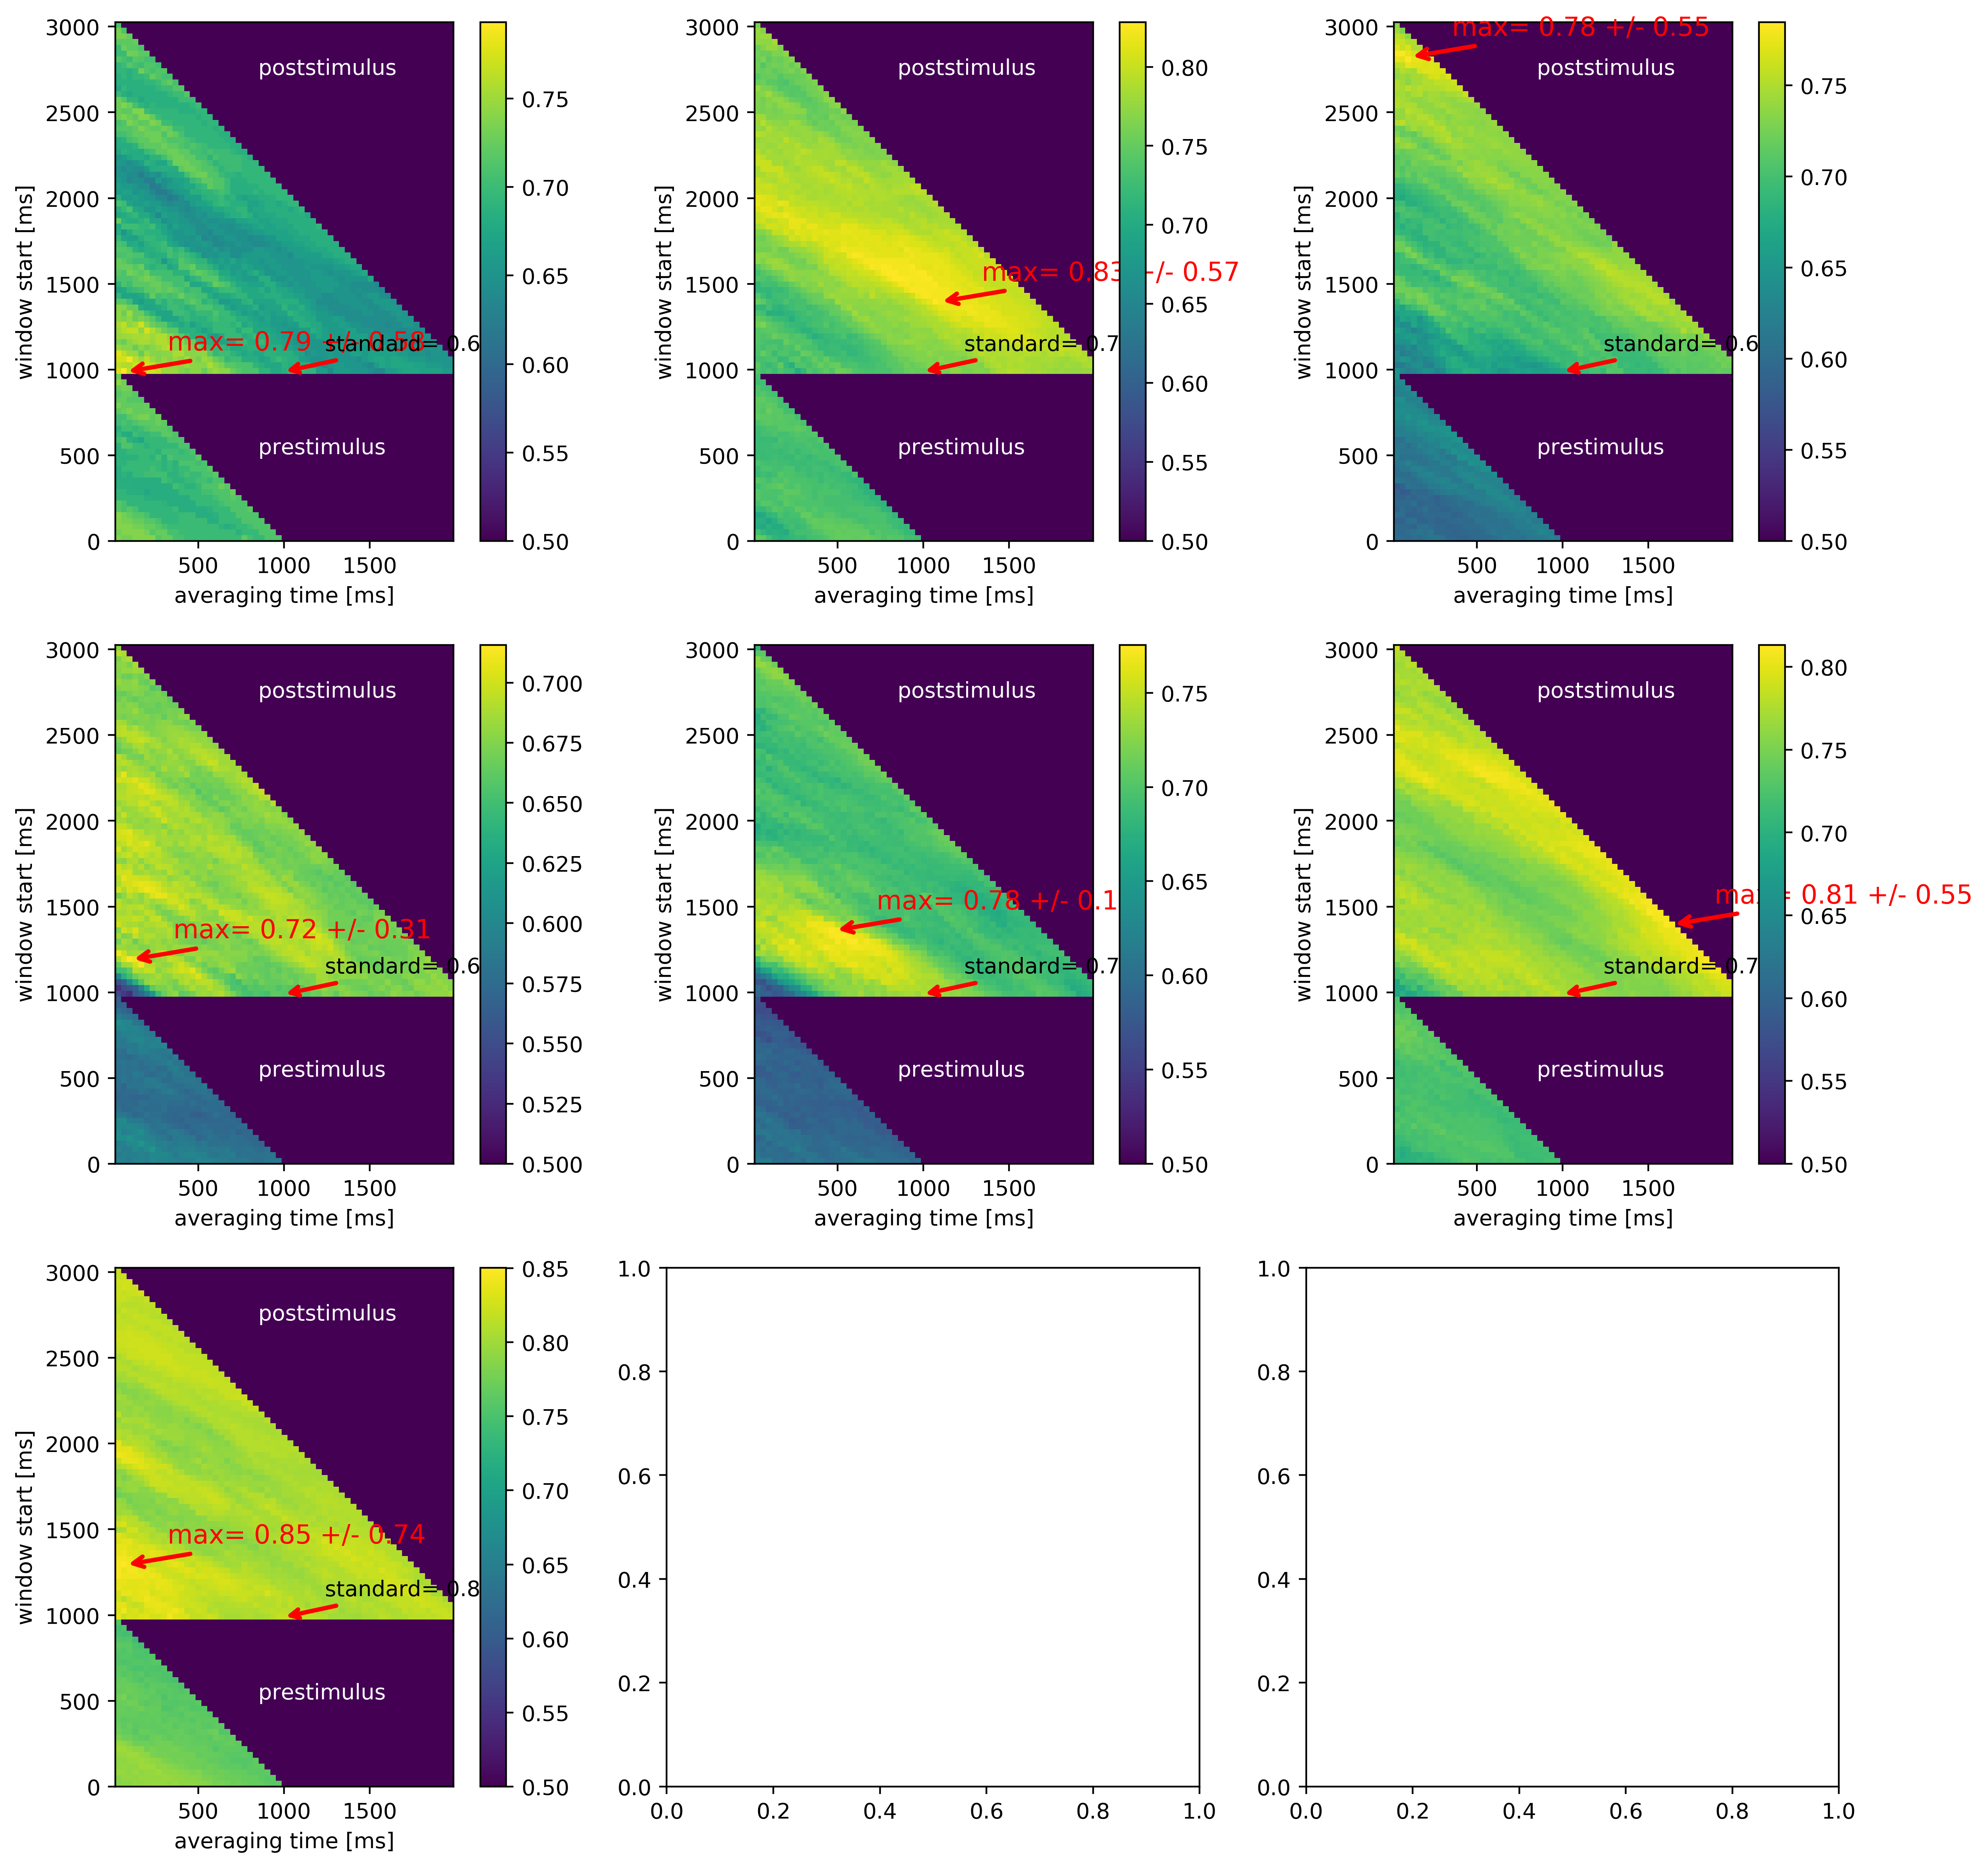
\includegraphics[width=0.6\textwidth]{placeholder_wind_hit.png}
	\end{figure}
	\end{center}
\end{frame}

\section{Population Coding}

\begin{frame}[fragile]{Population Coding - Idea (Mante, Sussillo 2013)}
\begin{center}
	\begin{figure}
      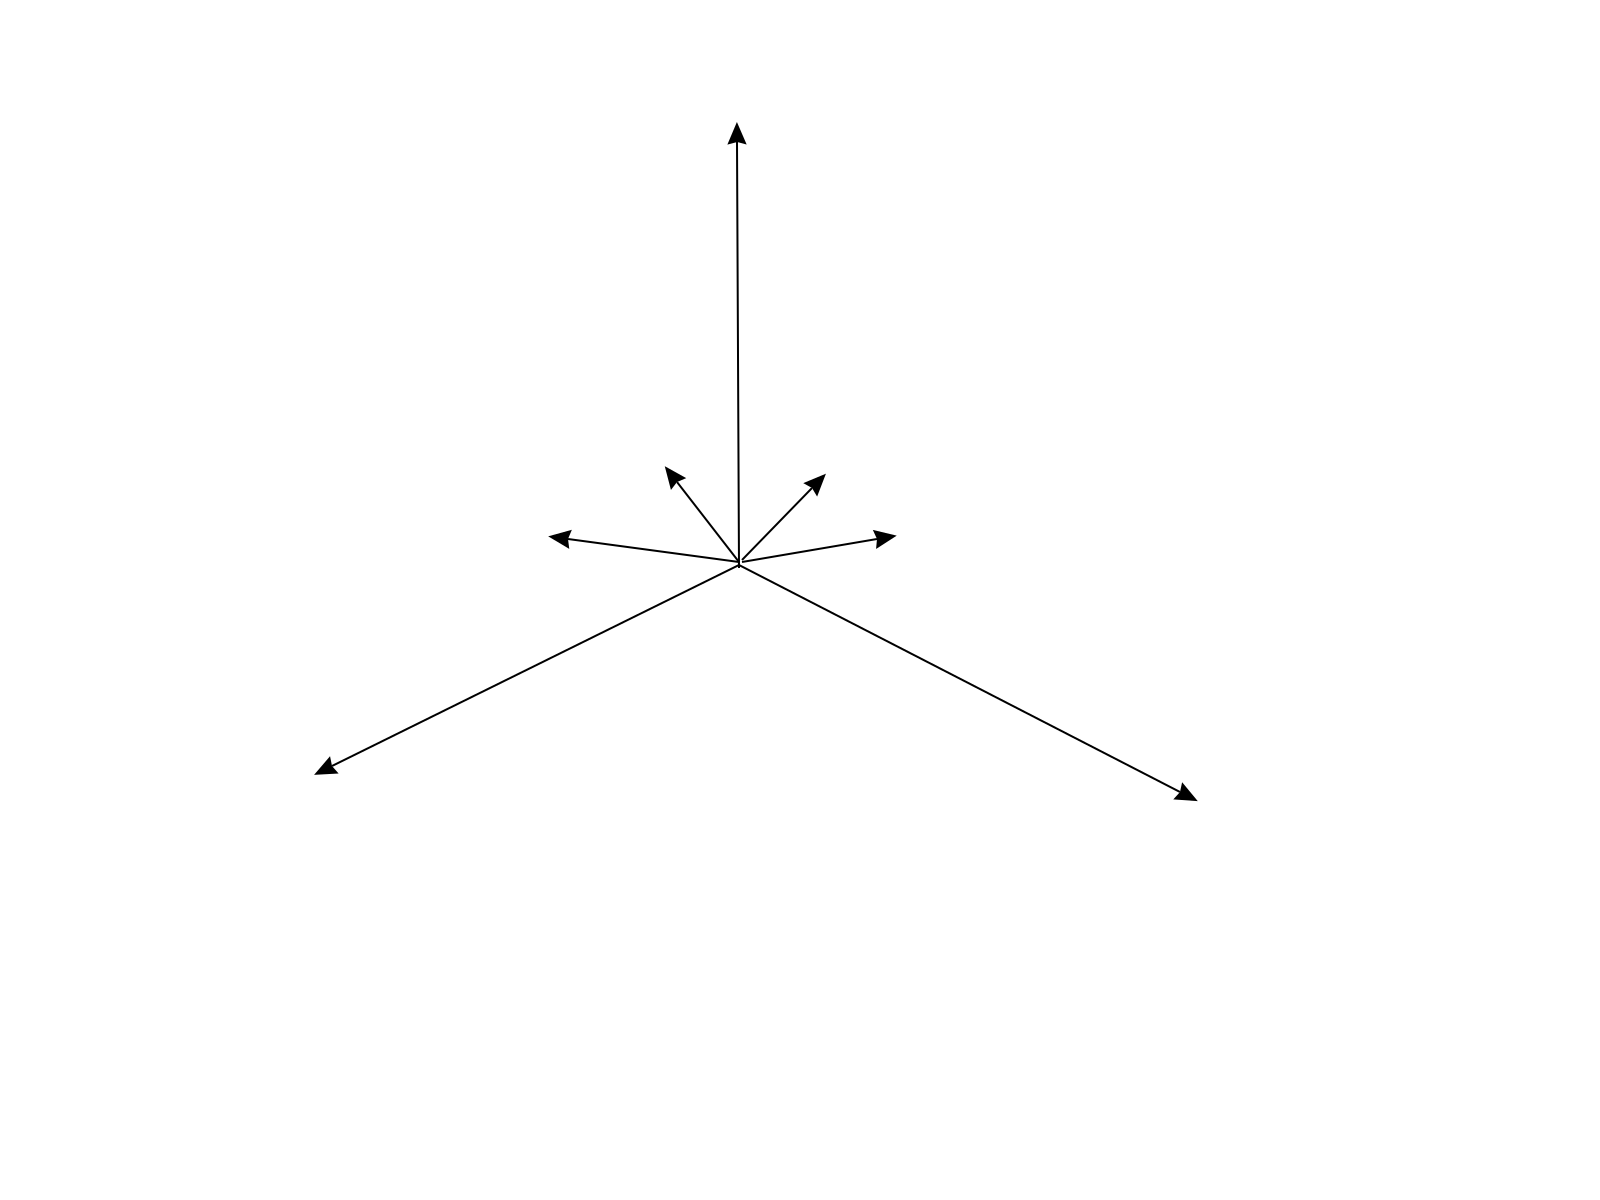
\includegraphics[width=1.0\textwidth]{coord.png}
	\end{figure}
	\end{center}
\end{frame}

\begin{frame}[fragile]{Population Coding - Idea (Mante, Sussillo 2013)}
\begin{center}
	\begin{figure}
      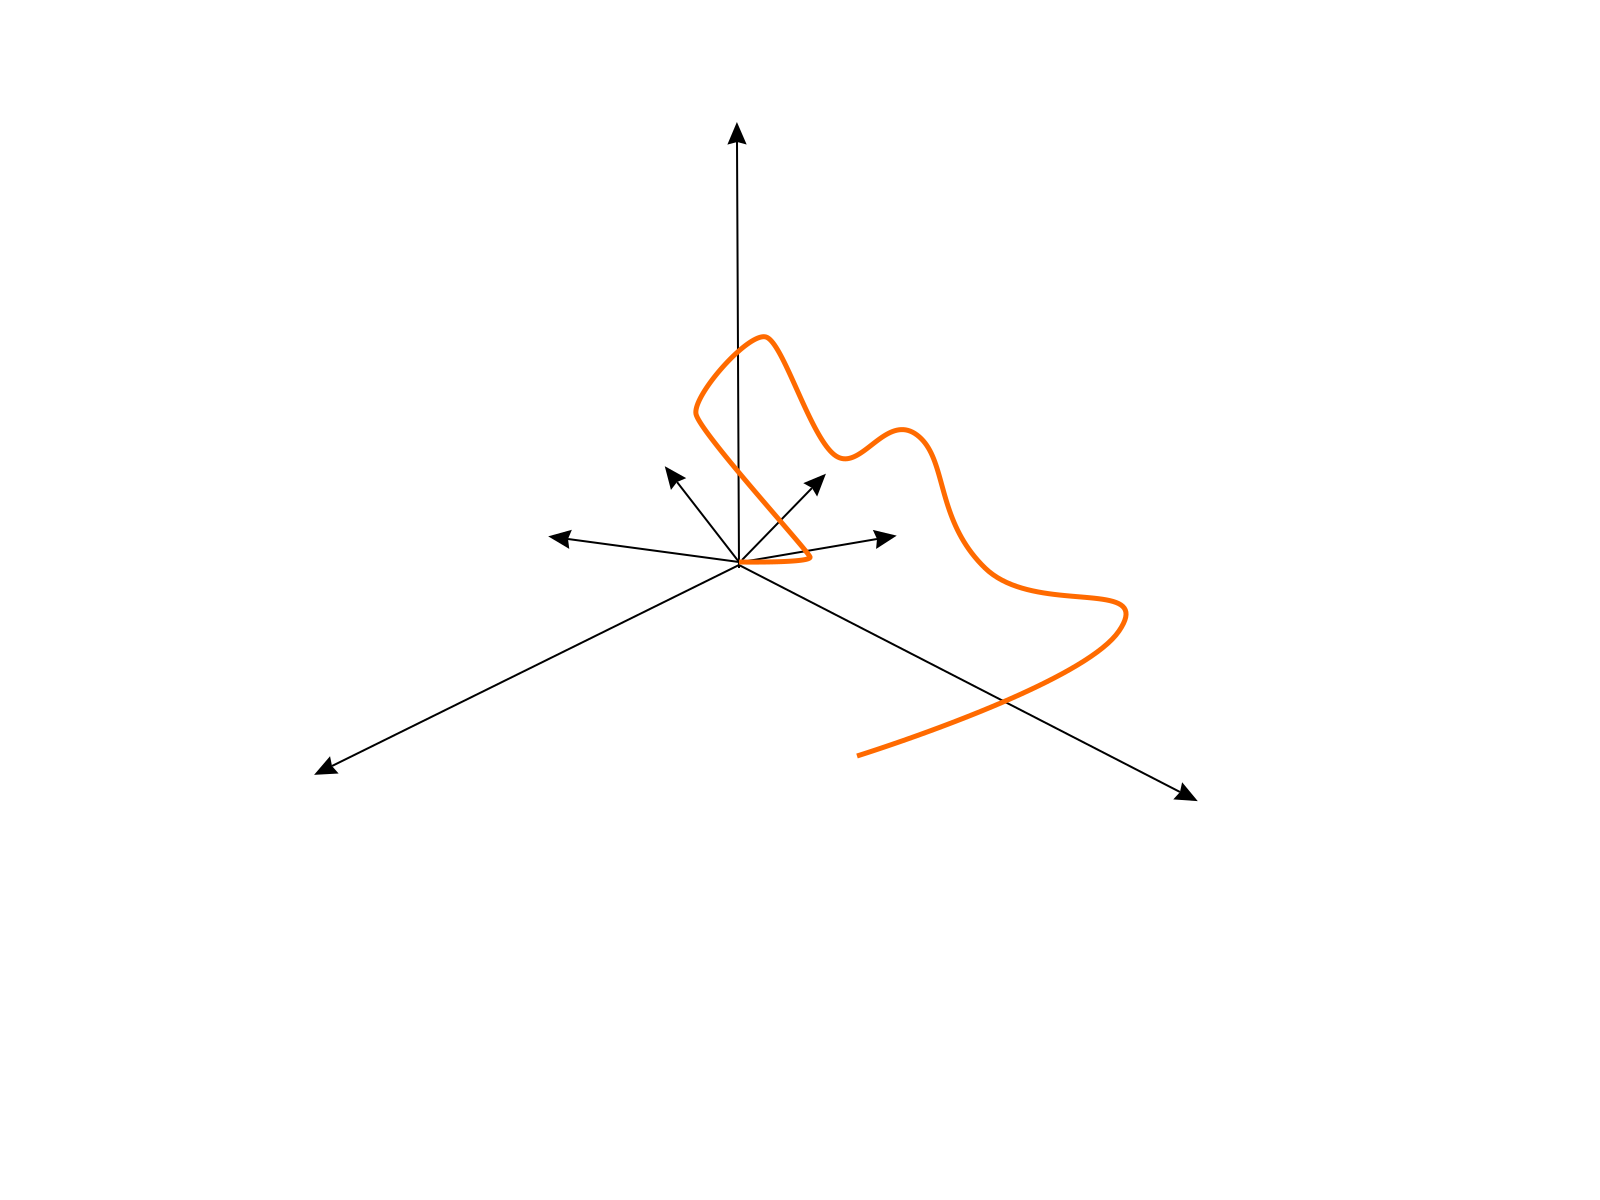
\includegraphics[width=1.0\textwidth]{traj.png}
	\end{figure}
	\end{center}
\end{frame}

\begin{frame}[fragile]{Population Coding - Idea (Mante, Sussillo 2013)}
\begin{center}
	\begin{figure}
      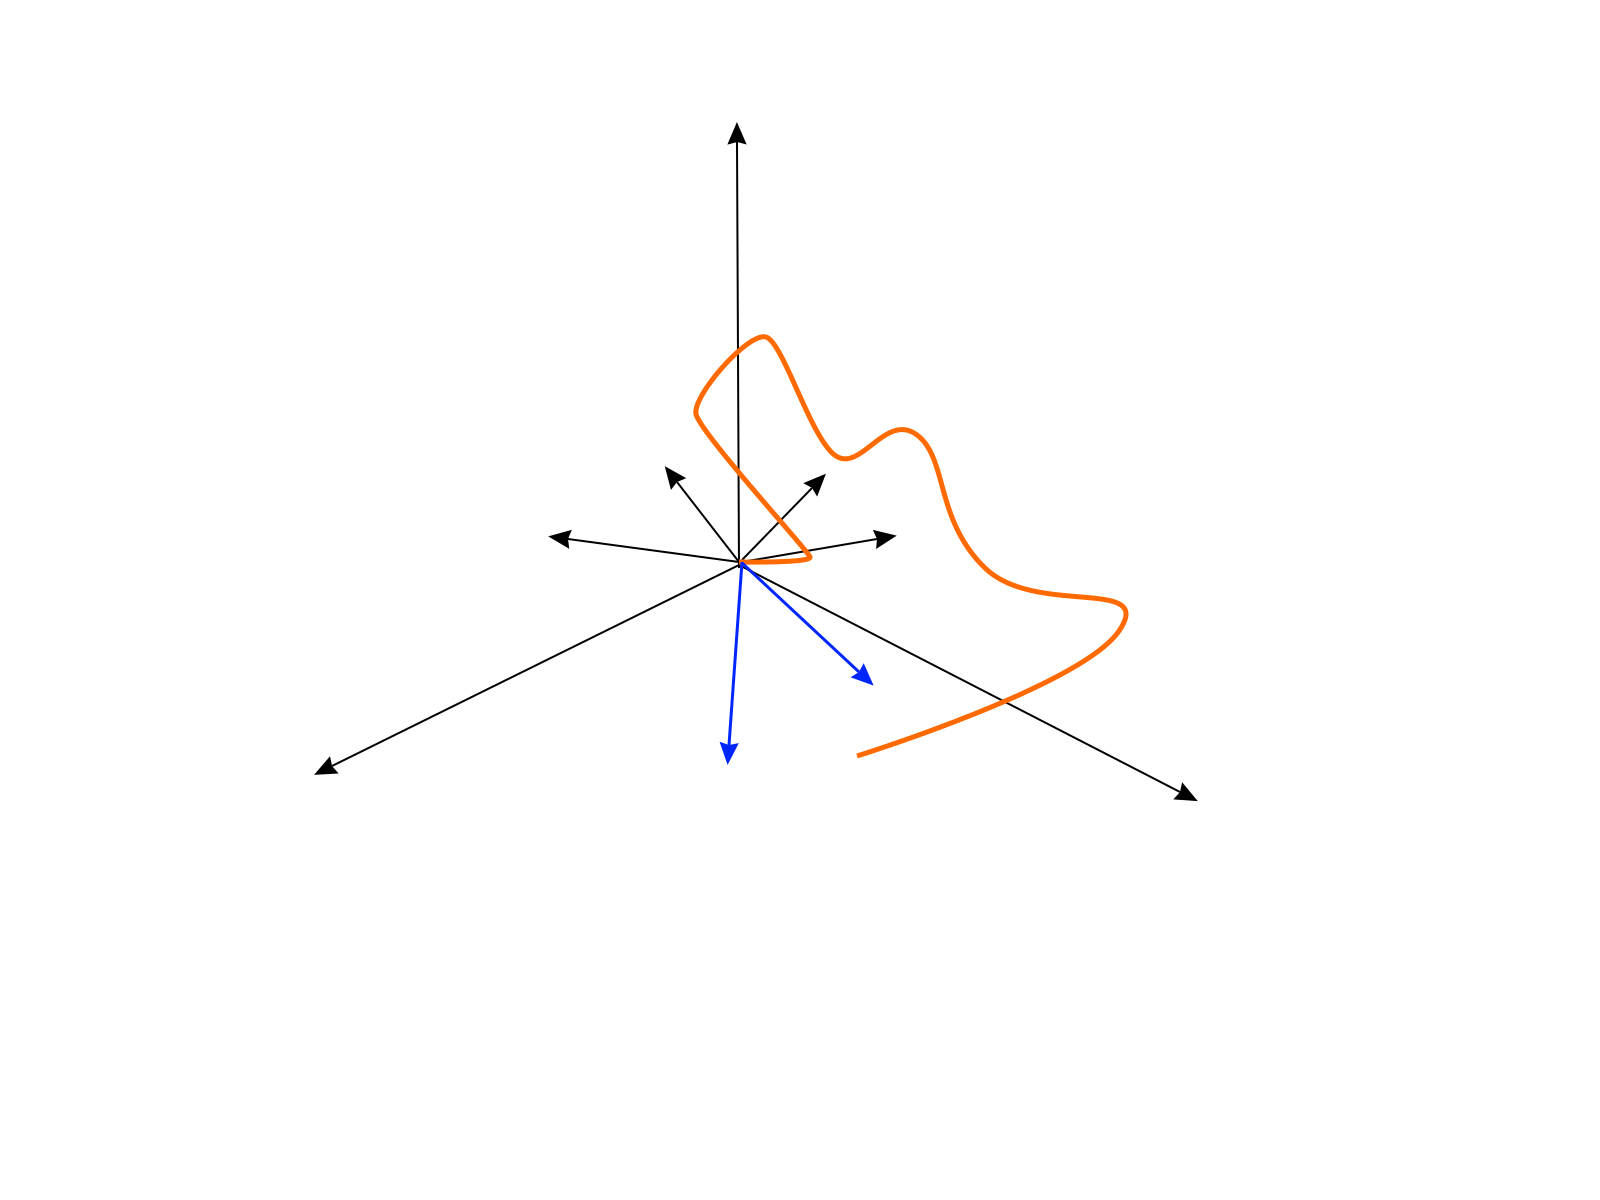
\includegraphics[width=1.0\textwidth]{new_coord.png}
	\end{figure}
	\end{center}
\end{frame}

\begin{frame}[fragile]{Population Coding - Idea (Mante, Sussillo 2013)}
\begin{center}
	\begin{figure}
      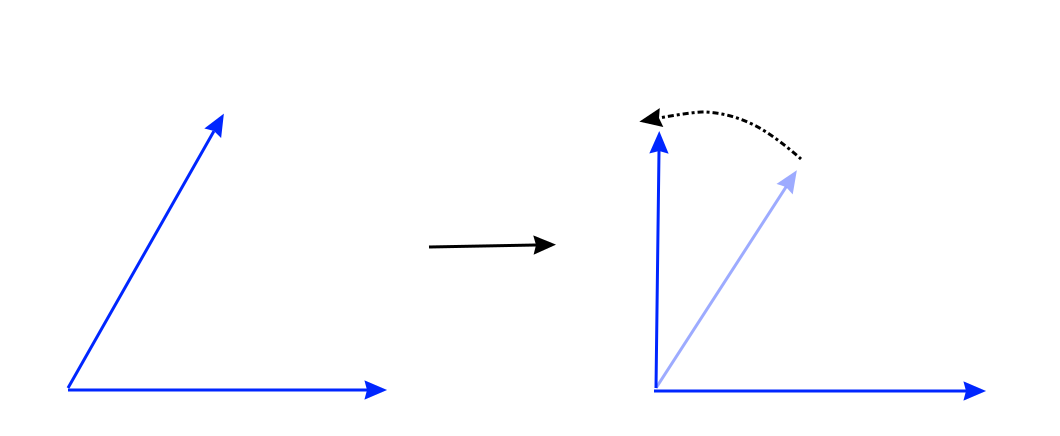
\includegraphics[width=1.0\textwidth]{trafo.png}
	\end{figure}
	\end{center}
\end{frame}

\begin{frame}[fragile]{Population Coding - Idea (Mante, Sussillo 2013)}
\begin{center}
	\begin{figure}
      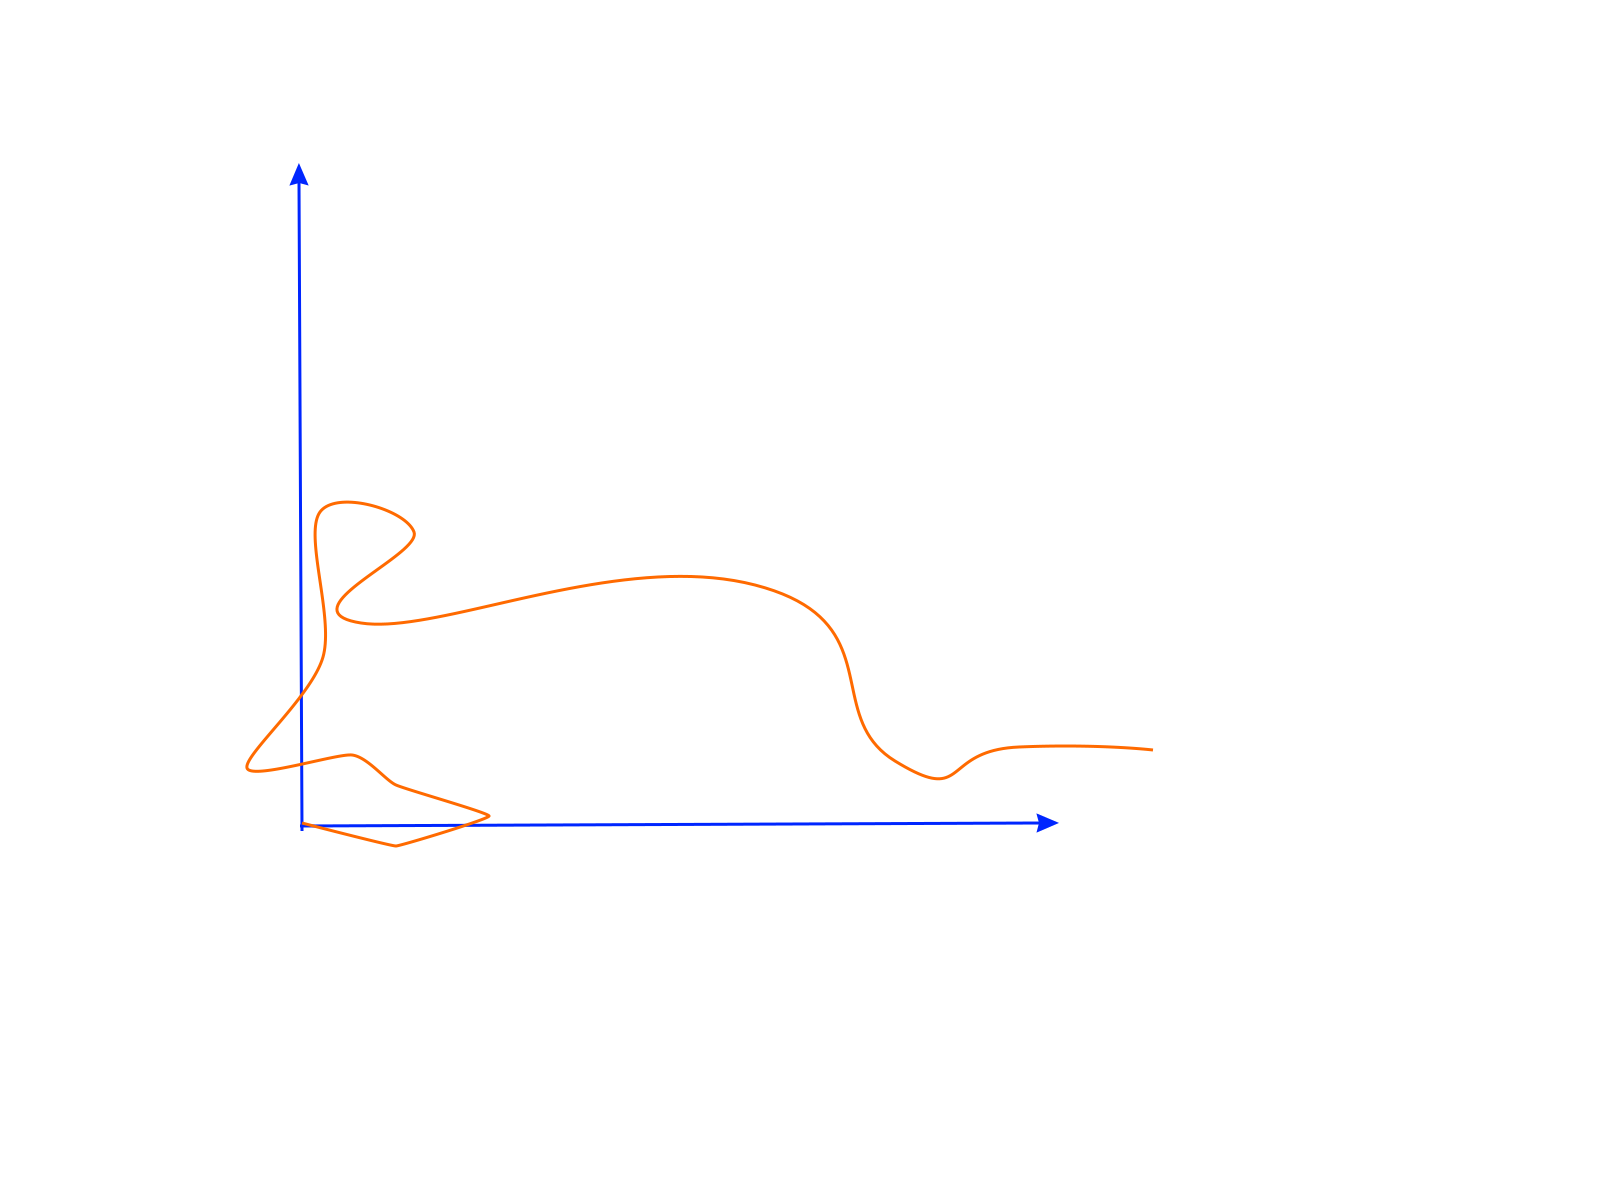
\includegraphics[width=1.0\textwidth]{trafo_final.png}
	\end{figure}
	\end{center}
\end{frame}

\begin{frame}[fragile]{Population Response in Task Variable Space}
\begin{center}
	\begin{figure}
	\caption*{Solve Problem with combined SVM first}
      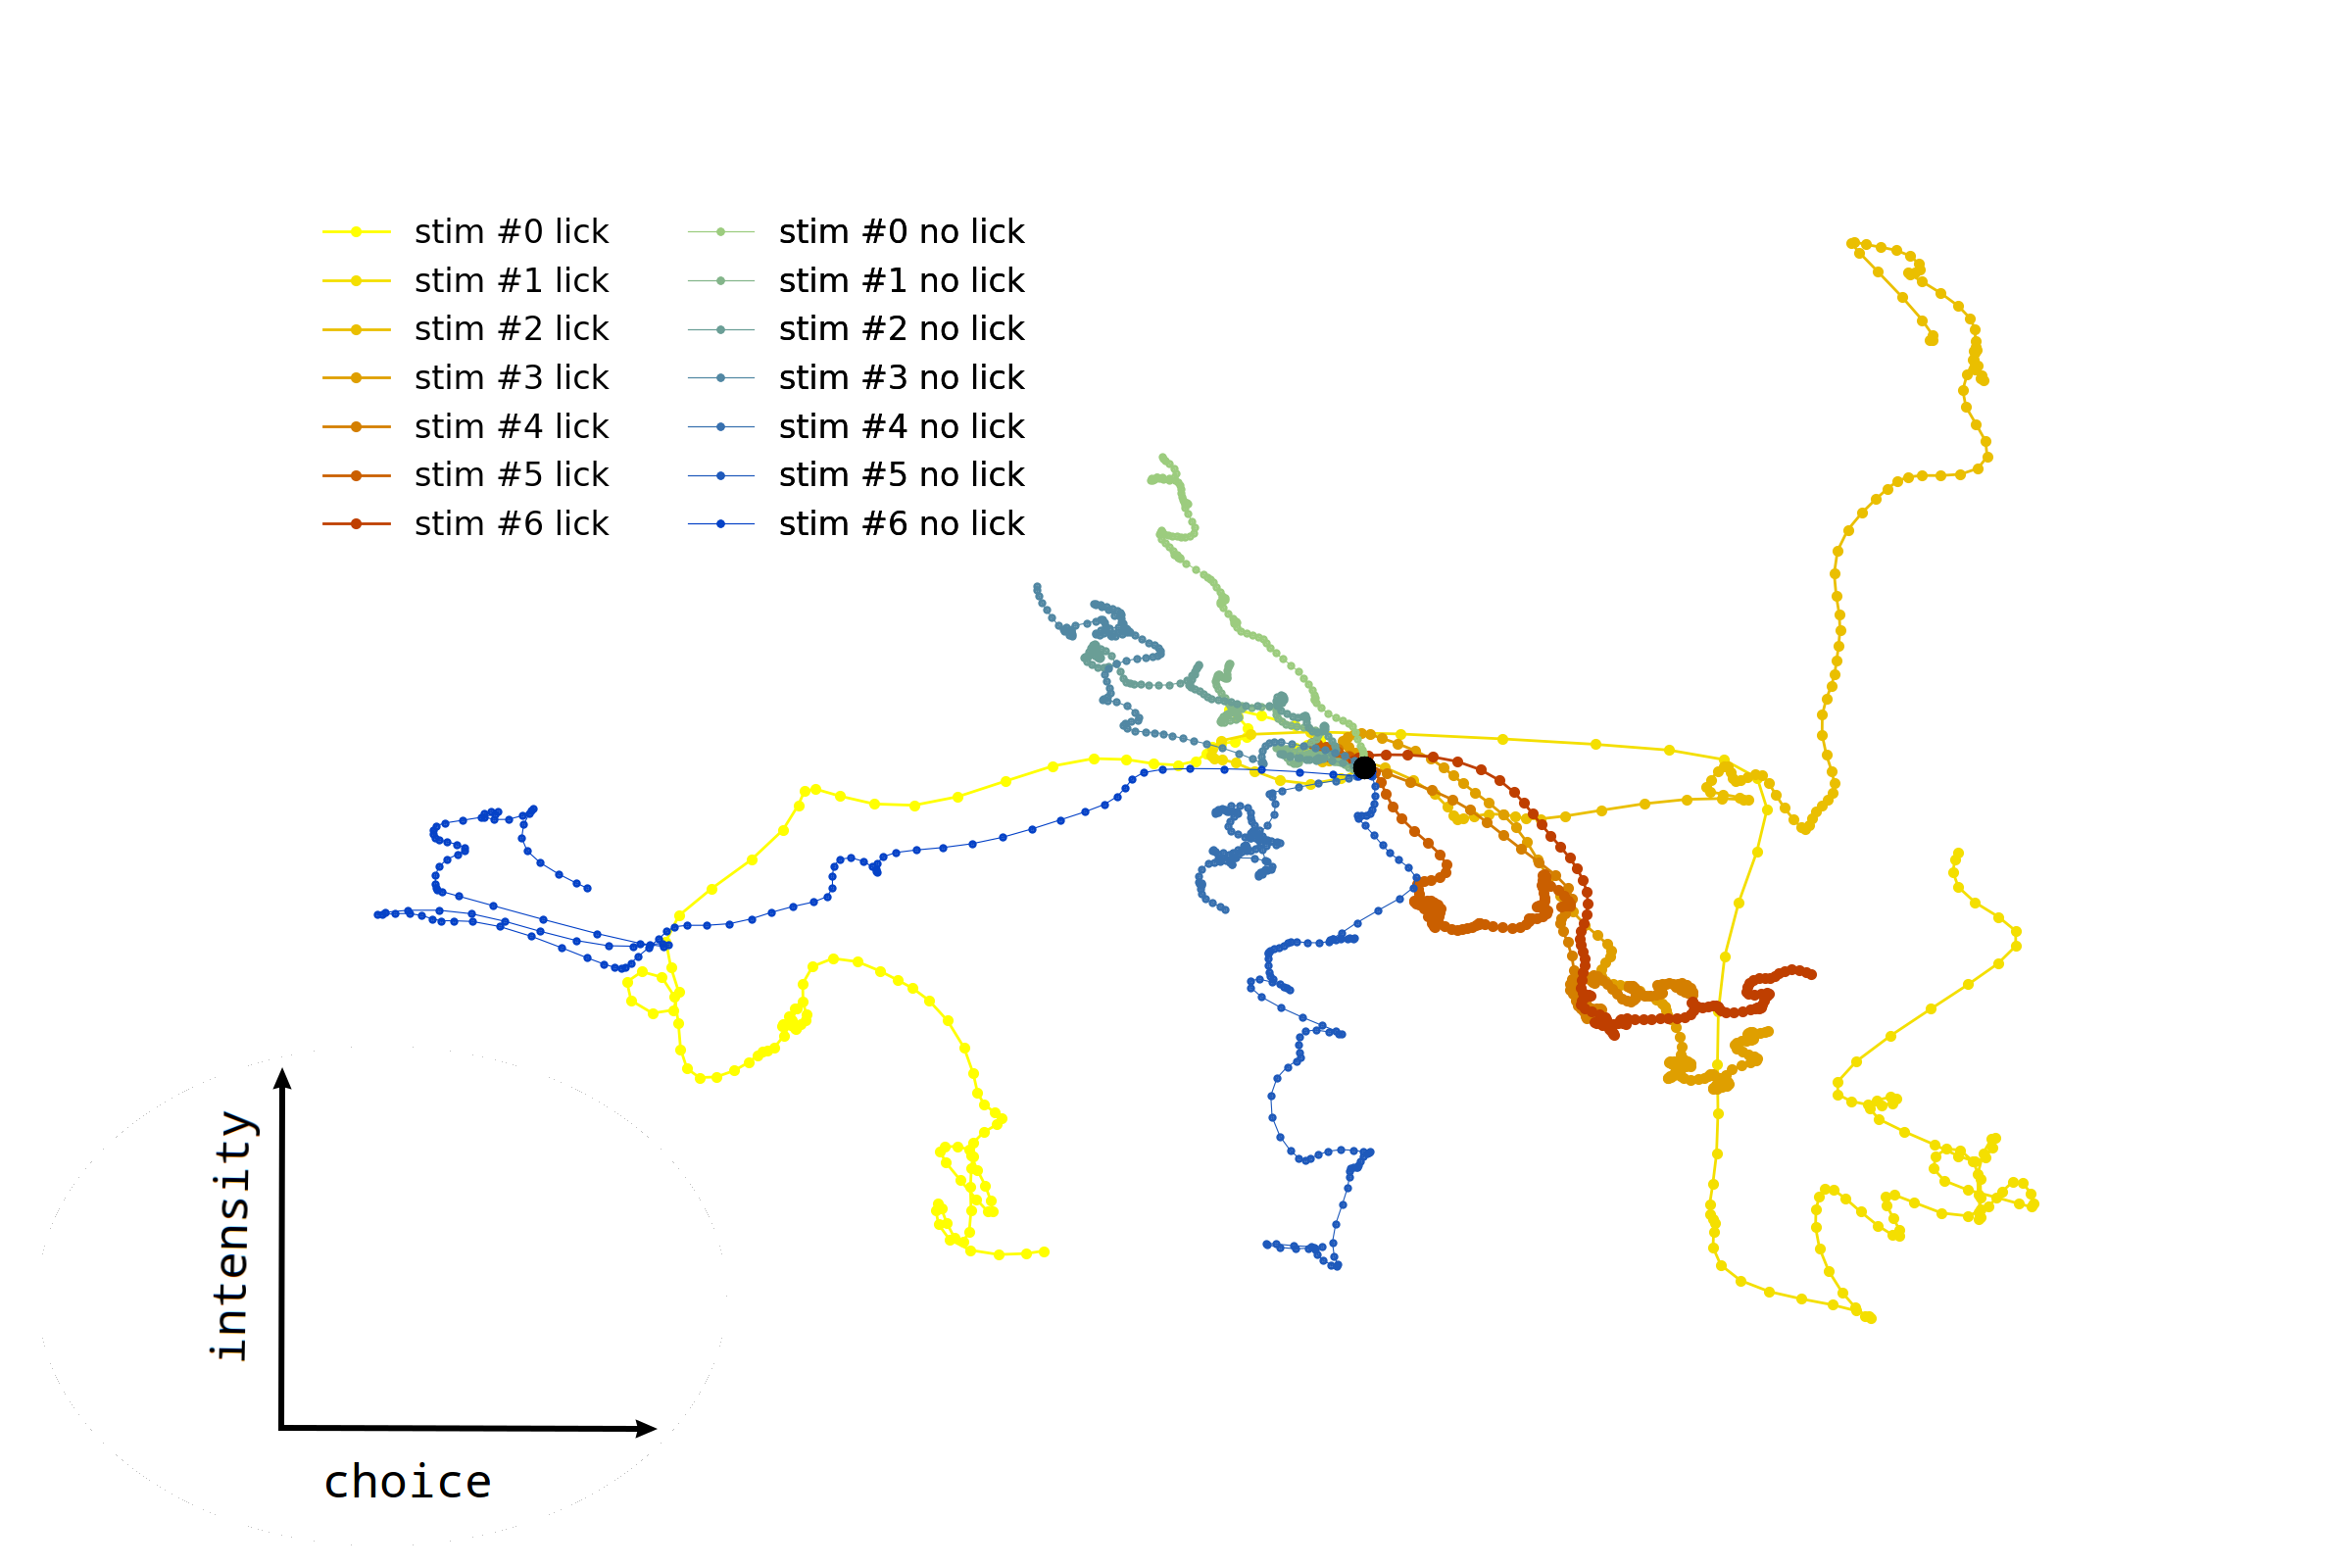
\includegraphics[width=0.7\textwidth]{reg.png}
	\end{figure}
	\end{center}
\end{frame}

\begin{frame}[fragile]{Population Response in Task Variable Space}
\begin{center}
	\begin{figure}
	\caption*{Solve Problem with combined SVM first}
      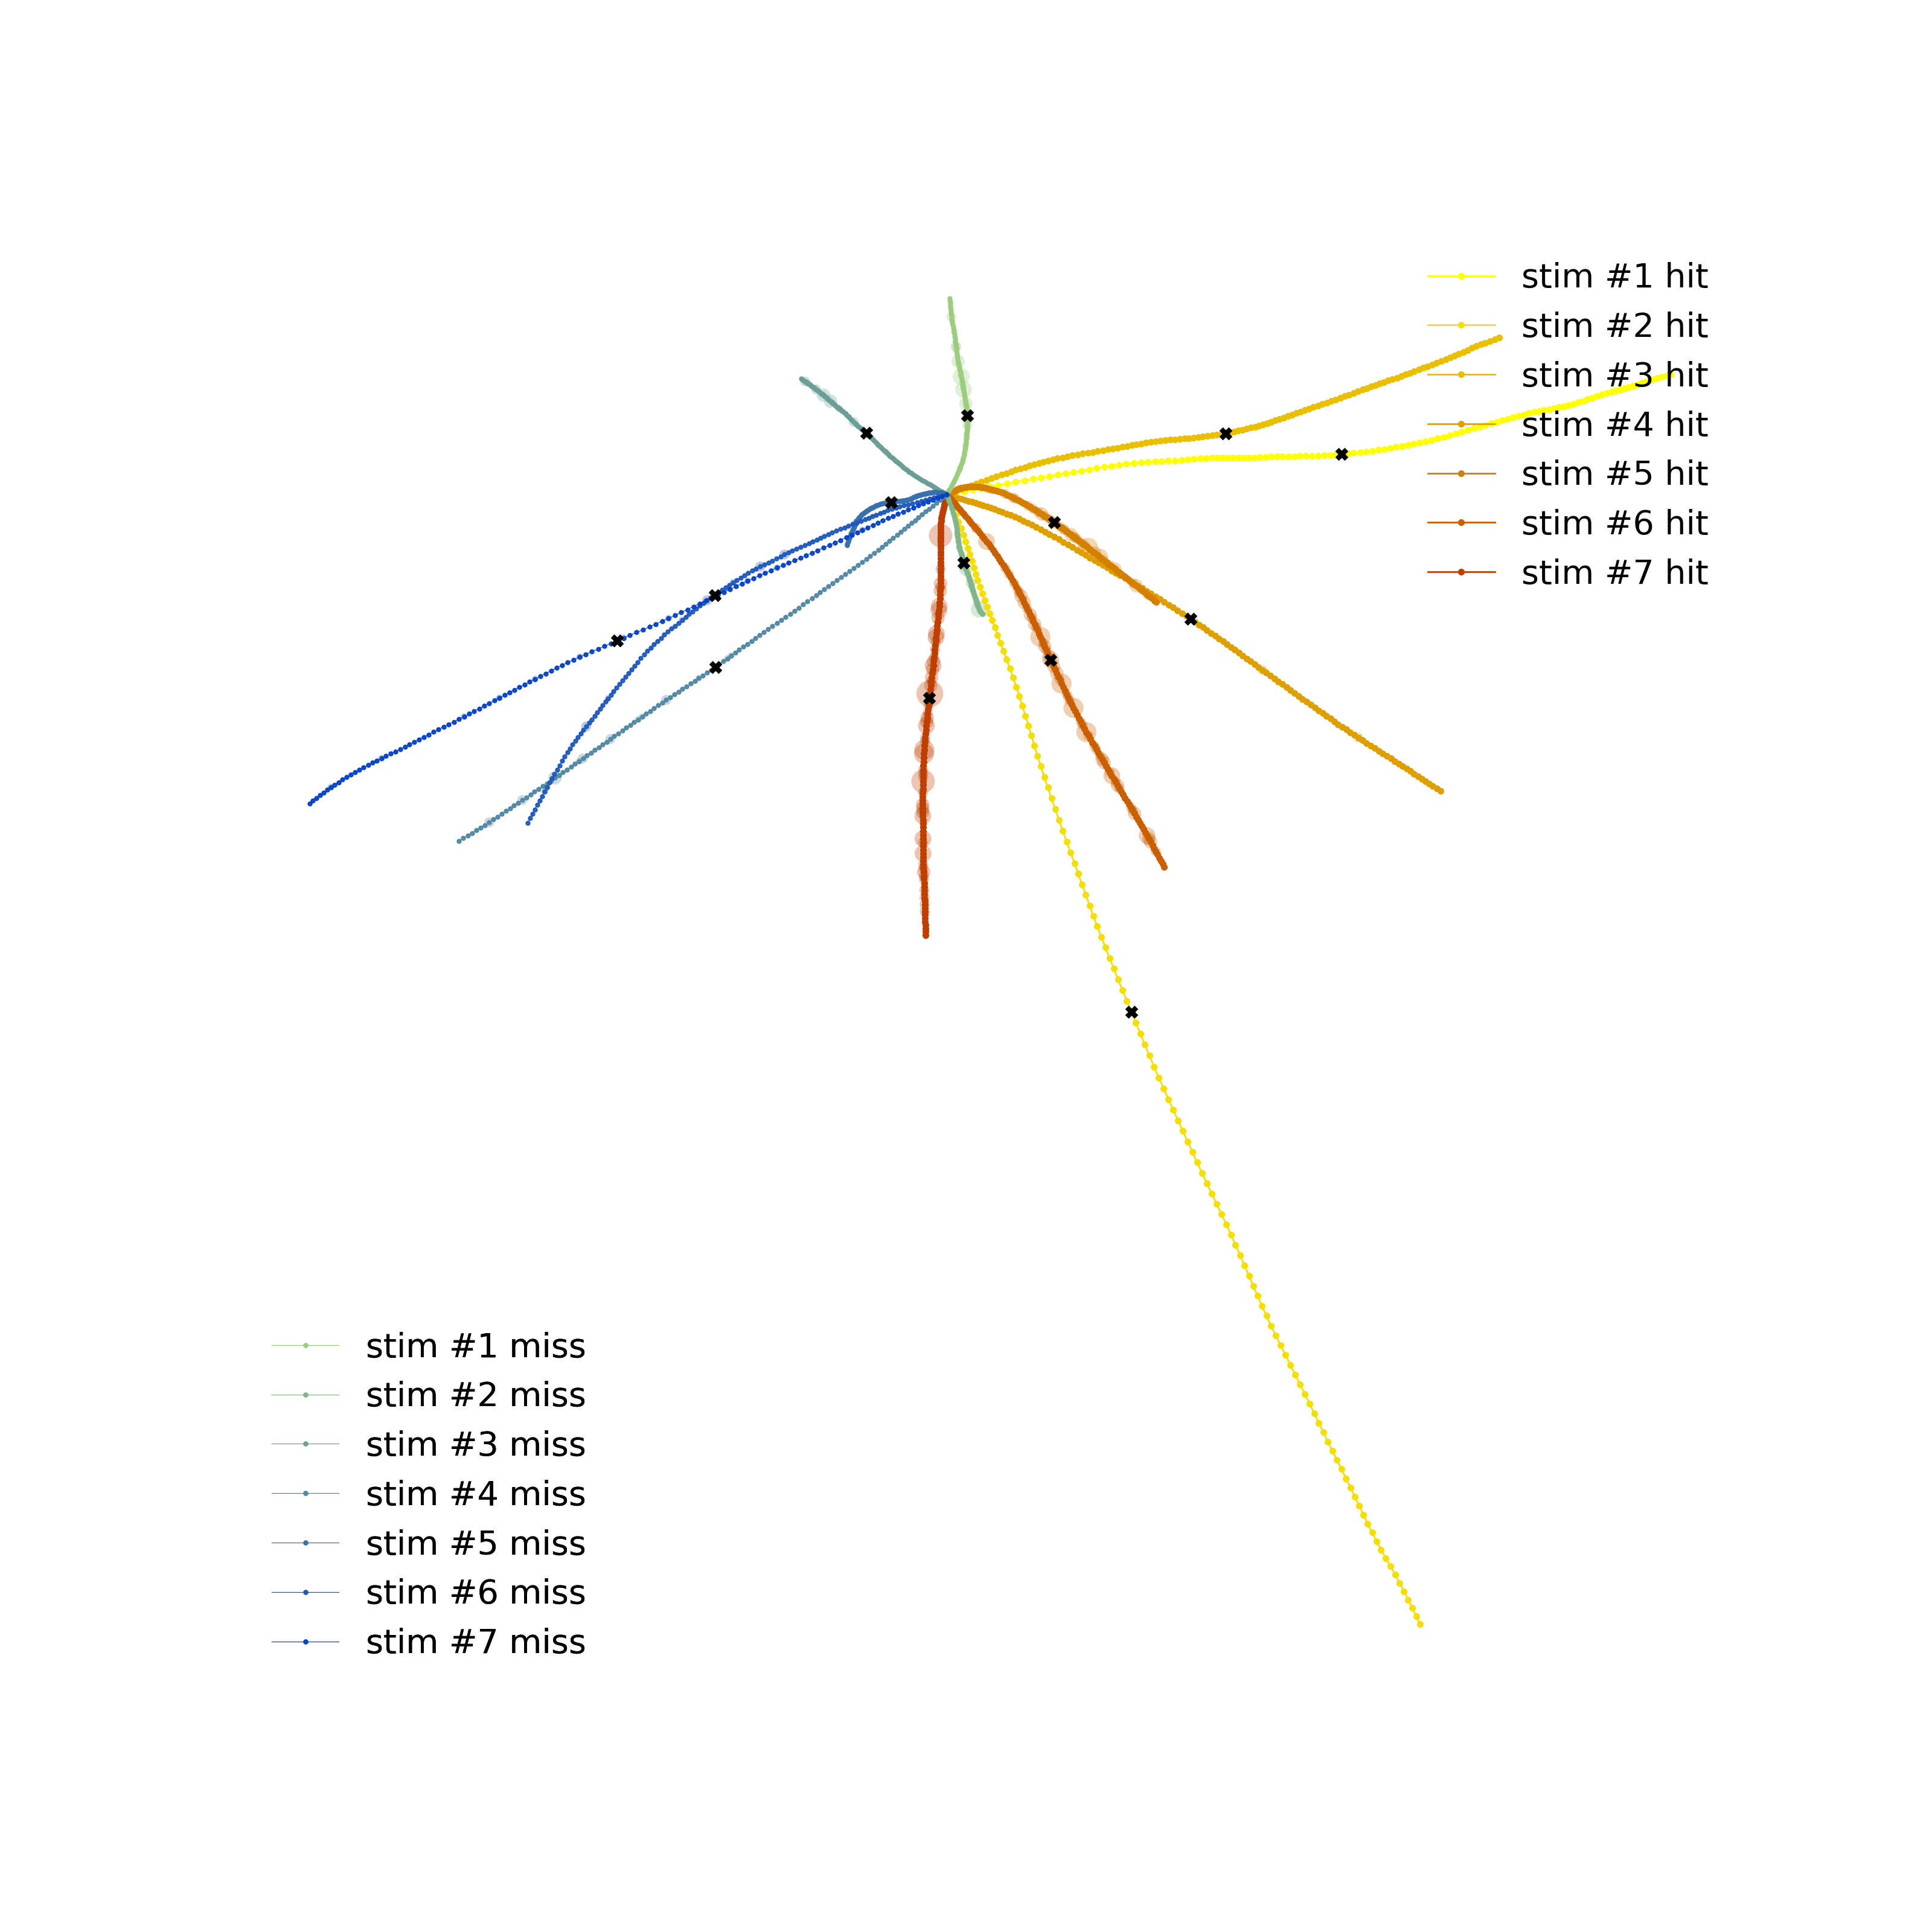
\includegraphics[width=0.7\textwidth]{reg_sum.png}
	\end{figure}
	\end{center}
\end{frame}

\begin{frame}
\begin{thebibliography}{9}
\bibitem {taka} Takahashi, N., Oertner, G. T., Hegemann, P. \& Larkum, E. M. Active cortical dendrites modulate perception. Science 335, 1587-1590 (2016)
\bibitem {mante} Mante V., Sussillo D., Shenoy KV., Newsome WT. Context-dependent computation by recurrent dynamics in prefrontal cortex. Nature 503, 78-84 (2013)
\bibitem {pinto} Pinto da Costa, J. New Results in Weighted Correlation and Weighted Principal Component Analysis with Applications, Chapter 2 (2015)
\end{thebibliography}
\end{frame}

\section*{Extra Slides}
\begin{frame}[fragile]{Weighted Rank Order Correlation Coefficient}
\only<+->{
We want to quantify the similarity between two rank orders of dendrites $R$ and $Q$, which both have length $n$.}

\only<+->{
Standard approach: Spearman's rank order coefficient 
$$
\rho(R,Q) = 1 - \frac{6\sum_i^nD_i^2}{n(n	^2-1)}
$$
where $D_i=R_i-Q_i$.}

\only<+->{
Problem: Many of the dendrites are not significant for classification but affect $\rho$ greatly. We would like to be able to \textbf{weight our} $\mathbf{D_i}$'s.}
\end{frame}

\begin{frame}[fragile]{Weighted Rank Order Correlation Coefficient}
\only<+->{
We want our rank order coefficient to be an affine linear function of $\sum_iw_iD_i^2$:

$$
\rho_W(R, Q) = A+B\sum_i^nw_iD_i^2
$$}
\only<+->{
If $R=Q$, we want $\rho_W=1$, and if the rankings are reversed, we want $\rho_W=-1$.}

\only<+->{
The first condition gives us $A=1$, and the second one
$$
B=\frac{-2}{\sum_i^nw_i(n-2i+1)^2} 
$$}
\only<+->{
Thus:
$$
\boxed{\rho_W(R,Q) = 1-\frac{-2\sum_i^nw_iD_i^2}{\sum_i^nw_i(n-2i+1)^2}}
$$}
\end{frame}

\begin{frame}[fragile]{Population Response in Task Variable Space}
\only<+->{
We would like to visualize the time evolution of the population response in a coordinate system in which the axes represent stimulus strength and choice.}

\only<+->{
To that end we use linear regression to write the normaized response of dendrite $i$ at time $t$ in trial $k$ as a linear combination of these task variables:
$$
r_k^{i,t} = \beta_1^{i,t}choice_k+\beta_2^{i,t}stimulus_k+\beta_3^{i,t}
$$}

\only<+->{
The regression coefficients $\beta_{\nu}^{i,t}$ describe how much the activity of dendrite $i$ at time $t$ in trial $k$ corresponds with variable $\nu$.}
\end{frame}

\begin{frame}[fragile]{Population Response in Task Variable Space}
We define
$$
\mathbf{F} = 
\begin{bmatrix}
choice_1 & ... & choice_n \\
stimulus_1 & ... & stimulus_n \\
1 & ... & 1
\end{bmatrix}
$$
and estimate for each dendrite $i$ and timepoint $t$
$$
\boldsymbol{\beta^{i,t}} = \mathbf{(FF^T)^{-1}Fr^{i,t}}
$$
\end{frame}

\begin{frame}[fragile]{Population Response in Task Variable Space}
\only<+->{
In total we have 14 conditions: 7 stimuli X two choices.}

\only<+->{
We define:
$$
\mathbf{x^{c,t}}
$$
as the (trial-averaged) population response to condition $c$ (for example lick at stimulus 1.00) at time $t$, which is a vector of $N_{unit}$ length.}

\only<+->{
The goal is to use $\boldsymbol{\beta}$ to find a two-dimensional subspace of the dendrite space into which we can transform $\mathbf{x^{c,t}}$.}
\end{frame}

\begin{frame}[fragile]{Population Response in Task Variable Space}
\only<+->{
We then use PCA to denoise the data matrix
$$
\mathbf{X}=
\begin{bmatrix}
 &  &  & \\
\mathbf{x_{c_1,t_1}} & ... & \mathbf{x_{c_1,t_n}} & ... & \mathbf{x_{c_m,t_n}}
\\
  &  &  &
\end{bmatrix}
$$}

\only<+->{
and we apply the denoising matrix to all $\boldsymbol{\beta^{\nu, t}}$ as well, which yields the denoised regression vectors
$$
\boldsymbol{\beta_{pca}^{\nu,t}}
$$}
\end{frame}

\begin{frame}[fragile]{Population Response in Task Variable Space}
\only<+->{
Since the $\boldsymbol{\beta_{pca}^{\nu,t}}$ are time variing but we would like a coordinate system that is fixed in time, we "freeze" them at the point in time at which there is maximum correlation:}
\only<+->{
\[
\boldsymbol{\beta^{\nu}_{max}}=\boldsymbol{\beta_{pca}^{\nu,t^{\nu}_{max}}}
\]
\[
t^{\nu}_{max} = argmax_t||\boldsymbol{\beta_{pca}^{\nu,t}}||
\]}
\end{frame}

\begin{frame}[fragile]{Population Response in Task Variable Space}
\only<+->{
We would like these $\boldsymbol{\beta^{\nu}_{max}}$ to be the basis vectors of our new coordinate system, however, they are not yet orthogonal.} 
\only<+->{We fix this by applying QR-decomposition to 
$$
\mathbf{B^{max}}=
\begin{bmatrix}
\mathbf{\beta^1_{max}} & \mathbf{\beta^2_{max}}
\end{bmatrix} = \mathbf{QR}
$$
where $\mathbf{Q}$ is an orthogonal matrix whose columns $\boldsymbol{\beta^{\nu}_{\bot}}$ are the \textbf{basis vectors} of our new coordinate system. We can now transform our data into it.}
\end{frame}

\end{document}
